%%%%%%%%%%%%%%%%%%%%%%%%%%
%%Preamble
%%%%%%%%%%%%%%%%%%%%%%%%%%
%\documentclass[11pt, A4]{report}
\documentclass[11pt, A4, oneside]{report}
\usepackage[a4paper, width=15cm, top=25mm, bottom=25mm, bindingoffset=6mm]{geometry}

%%%%%%%%%%%%%%%%%%%%%%%%%%
%%Preamble
%%%%%%%%%%%%%%%%%%%%%%%%%%
\usepackage[utf8]{inputenc}
\usepackage[T1]{fontenc}
\usepackage[english]{babel}
%\renewcommand{\chaptername}{}
\usepackage{titlesec}
\titleformat{\chapter}[hang]{\huge\bfseries}{\thechapter{. }}{0pt}{\huge\bfseries}

%use biblatex with natbib
\usepackage[style=apa, sorting = nyt, natbib]{biblatex}
%\usepackage[style=apa, maxnames=1, sorting = nyt, natbib]{biblatex}
\addbibresource{Bibliography.bib}
\addbibresource{R-cite.bib}
\addbibresource{news.bib}
\addbibresource{articles_ext.bib}
%\bibliographystyle{apalike}

%package to create hyperlinks
\usepackage[hidelinks]{hyperref}

%no indents with new paragraphs and set gap length
\setlength\parindent{0pt}
\setlength{\parskip}{0.5\baselineskip}

%graphics and tikzipictures
\newenvironment{rotatepage}%rotate pdf page
    {\clearpage\pagebreak[4]\global\pdfpageattr\expandafter{\the\pdfpageattr/Rotate 90}}%
    {\clearpage\pagebreak[4]\global\pdfpageattr\expandafter{\the\pdfpageattr/Rotate 0}}%
    
\usepackage{graphicx}
\usepackage{tikz}
\usetikzlibrary{shapes.geometric, arrows}
\tikzstyle{startstop} = [rectangle, rounded corners, minimum width=3cm, minimum height=1cm,text centered, text width=3cm, draw=black]%, fill=red!30
\tikzstyle{io} = [trapezium, trapezium left angle=70, trapezium right angle=110, minimum width=2cm, minimum height=1cm, text centered, text width=2.7cm, draw=black]%, fill=blue!30
\tikzstyle{process} = [rectangle, minimum width=3cm, minimum height=1cm, text centered, text width=3cm, draw=black]%, fill=orange!30
\tikzstyle{decision} = [diamond, minimum width=3cm, minimum height=1cm, text centered, text width=3cm, draw=black]%, fill=green!30
\tikzstyle{arrow} = [thick,->,>=stealth]

%smaller graphics captions
%\usepackage{caption}
%\captionsetup{font=footnotesize} % reduce size of caption because text is 11
\usepackage[font=small,labelfont=bf]{caption}

%options for page rotation 
%\usepackage[final]{pdfpages}
\usepackage{pdfpages}
\usepackage{multirow}
\usepackage{lscape}
\usepackage{rotating}

%math pacages
\usepackage{float}
\usepackage{mathtools}




%packages to use helvetic sserif for headings
%from here: https://graphicdesign.stackexchange.com/questions/46663/is-computer-modern-a-high-quality-font
%if i use this need to change appearance in the TOC
%    \usepackage{cmlgc,amssymb,amsmath}
%      \DeclareTextCommandDefault{\textbullet}{\ensuremath{\bullet}}
%    \usepackage[scaled]{helvet}
%\usepackage[T1]{fontenc}
   % ⋮
%    \usepackage{sectsty}
%      \allsectionsfont{\sffamily\raggedright}
  
\setcounter{secnumdepth}{1}
%% remove number of subchapters

\begin{document}

\begin{titlepage}

%logos

\includegraphics[width = 0.4\textwidth]{A_Pre/A_img/eth_logo_kurz_pos.eps}
\hspace{2cm}

\includegraphics[width = .2\textwidth]{A_Pre/A_img/PLUS_logo.jpg}

\hspace{8cm}
\includegraphics[width = .3\textwidth]{A_Pre/A_img/fcl_tana_logo_2.png}

\begin{center} 
\vspace{1cm}    
%    \par\noindent\rule{\textwidth}{0.4pt}\\
\vspace{.5cm} 

\Huge
    \textbf{Is urban growth eating up blue and green infrastructure?}\\ %in southern cities?
\vspace{1cm}
\Large 
    Using remote sensing to identify areas backfilled with soil and study drivers of their distribution in Antananarivo\\
    
\vspace{.5cm}
%    \par\noindent\rule{\textwidth}{0.4pt}\\  
 
\vspace{2cm}    
\large    
    \textbf{Author:}\\
    Carl A. Joseph\\ 
    16-052-409\\
\vspace{1cm}   
    \begin{minipage}{5cm}
        \textbf{Supervisor:}\\
        Prof. Dr. Adrienne\\ Grêt-Regamey\\
        \textit{ETH Zürich}\\
            %\vspace{0.5cm}
    \end{minipage}
    \begin{minipage}{5cm}
        \begin{flushright}
            \textbf{Co-Supervisors:}\\
            Dr. Maarten J. v Strien\\
            \textit{ETH Zürich}\\
            Dr. Nicolas Salliou\\
            \textit{ETH Zürich}\\
        \end{flushright}
    \end{minipage}
       % \end{tabbing}

\vspace{3cm}
\centering
    Master's Thesis\\
    Master's degree programme in Environmental Sciences

\vspace{1cm}
    12 September 2022\\

\end{center}
\end{titlepage}

\phantomsection\addcontentsline{toc}{chapter}{Acknowledgements}
\chapter*{Acknowledgements}
\pagenumbering{roman}
%Adrienne, thanks for feedback at presentations etc.
I thank my Co-Supervisors Nicolas Salliou and Maarten van Strien for all their help and support whilst working on my thesis. In terms of expert knowledge on the region of Antananarivo and of making contacts to other experts in the region, or concerning relevant topics, Nicolas' help was essential for me. Thanks to Maarten I felt supported in diving into a new topic and approach, by learning to work with Google Earth Engine and remote sensing data, knowing that I would always be able to get help. I would like to thank Adrienne
Grêt-Regamey for mentoring the thesis and providing feedback during the presentations. Many thanks to Bruno Ramamonjisoa for taking his time during two long sessions to answer my questions on backfilled areas in Antananarivo, thus helping me in gaining more data for training and validating my models.
Many thanks to the PLUS group for taking me in and providing me with a workspace during my master's thesis.
Further thanks go to friends and family, who helped me with corrections, critical questions, and proofreading.

\newpage
\phantomsection\addcontentsline{toc}{chapter}{Abstract}
\chapter*{Abstract}
Urban growth in southern cities has the potential to affect Blue and Green Infrastructure (BGI), reducing its protective functions which benefit  society. In the case of Antananarivo, the capital of Madagascar, the growth of the city toward its surrounding plains under rice cultivation is a controversial issue, and little data is available on the magnitude of this process. A key step in the land use transition from BGI like rice fields to urban and built-over land is filling it up with earth (backfilling), to create an even surface above the water level. In terms of urban planning, sustainable city development and risk management, a quantitative assessment of this process taking place would be useful.\\
In this study, we identified such backfilled areas and 13 other land use/ land cover (LULC) classes in the Greater Antananarivo region over a time-series of 10 years (2013 - 2022), using a supervised Random Forest classification model in Google Earth Engine  on USGS Landsat 8 satellite images (30 m resolution). The resulting yearly LULC maps were used to calculate and display the yearly increase in backfilled surface in the study area. Binary logistic regression was used to investigate the influence of different variables, originating from our data set and external sources, on the spatial distribution of newly occurred backfills.\\
The average annual increase of backfilled areas was 0.76 km$^2$year$^{-1}$, whereby no significant linear trend over the examined time period was observed. Using information on the classification of pixels in the previous year, a conversion rate of 0.51 km$^2$year$^{-1}$ from BGI to backfilled area was achieved. The fit of the logistic regression model, when using data of all time steps combined, is described by a Mc Fadden's pseudo R$^2$ of 0.11. When run only on the data concerning LULC information of the year the classification was trained on and the backfill distribution of the year after, the model fits with an R$^2$ of 0.34. In both cases, the most important independent variable was the distance to backfilled areas in the previous year, with odds ratios (OR) below one, meaning that the probability for new backfills decreased with a unit increase in distance [hm] to backfilled areas in the year before (all years: OR 0.93, 95\% Confidence Interval [0.93, 0.94] | training year: OR 0.68, 95\% Confidence Interval [0.64, 0.72]).\\
The calculated backfill area increase and conversion rates are low (<0.3 \%year$^{-1}$), considering the size of the study area of 274.5 km$^2$, of which a large fraction is made up by BGI. Based on this data, the risk of city expansion at expense of BGI is currently not alarming. It is not clear how this relates to the controversy concerning backfilling, which could also be a sign of awareness about the issue, leading to caution. The regression analysis indicates a positive relationship between new backfills and the proximity to existing ones. Combined with the information evident in backfill increase maps, this indicates a tendency of backfills to grow over multiple years, or occur in proximity to each other. This is especially clear in years with a higher model fit. The model fit and ratios for different variables differed very strongly when looking at the years separately, explaining the low overall fit. The association of backfills to other classes differs between years and there might be variables not represented by this model, which play an important role for the occurrence and distribution of new backfills. The difference between the years could be indicative of different kinds of backfills having varying characteristics. For instance, large filled up areas that are to be built over for industrial purposes can be expected to occur in different patterns, than  backfills that are used to later build roads upon, both of which were recognized by the supervised classification model.\\
As could be expected Backfilled areas often occur in proximity to each other. In a future analyses, it would be important to distinguish different types of backfilled areas, since they are likely to differ in key characteristics.  The rate of BGI loss at the expense of backfilling is currently low in the plains surrounding Antananarivo. Further research would be needed to look into reasons for this, which could provide beneficial knowledge for future planning. %where distribution could be beneficial to identify areas at risk amd maybe lessen the incentive of owners to backfills if it is a decision driver by e.g. lack of options or farming income.

%The results showed an increase in backfilled area that was lower than expected. Our data indicates that in the case of Antananarivo, the loss of BGI due to expansion of the city and thus also the coinciding risks are currently low. 

%why is the issue controversial if the impact is so small? -->maybe its the otehr way around and the impact is small, because it is controversial

%in future it might be interesting to get infomation on how long backfills normally stay barren

%further investigationconcerning socoeconomic independent variables like land zoning, prices, ownership etc. might be iinsightful for driver and prediction analyses




%\newpage
%\phantomsection\addcontentsline{toc}{chapter}{Abbreviations}
%\chapter*{Abbreviations}
%
%\begin{description}
%   \item[BGI] Blue and Green Infrastructure
%   \item[GEE] Google Earth Engine
%   \item[LULC] Land use / land cover
%   \item[TD] Training Data
   
%\end{description}

\newpage
%\chapter*{Contents}
\renewcommand*\contentsname{Contents}
\bgroup
%\fontfamily{phv}\selectfont
\tableofcontents
\egroup

\newpage
\chapter{Introduction}
\pagenumbering{arabic}
Urbanization and population growth are currently pressing issues on a global scale. The fraction of population residing in urban places is steadily increasing, especially for African regions, and predicted to further do so up to (at least) 2050 (\cite{united2012world}). In African cities, a growing demand for living space and other infrastructure often leads to urban sprawl, as cities expand toward the surrounding areas (\cite{Shao.2021, Xu.2019}).%define urban sprawl
%urban expansions negative effects
This rapid expansion can have various negative effects, ranging from declines in ecosystem services of the surrounding land, to lower living quality, and air pollution (\cite{Shao.2021}).

The city of Antananarivo, the capital of Madagascar, is also currently undergoing its urban transition. It is a city that grew on inhabited hills surrounded by lowlands, which are often subject to flooding and widely used for rice cultivation. Since the city is surrounded by agricultural land uses, its expansion often comes at the expense of the latter (\cite{Aubry.2012, Dupuy.2020b}). 
%urban agriculture food security
The agricultural area surrounding Antananarivo, a large part of which is made up of rice fields, plays a substantial role in the food supply for the population, especially for farming households or people with a lower income. Consistently, almost a quarter of all households in the region are involved in urban agriculture, most of which are households in the agglomeration of the city, rather than it's urban core (\cite{Dupuy.2020b}). Both these factors highlight the importance of urban agriculture in Antananarivo for food supply and income of households in the agglomeration. %there are also larger farms (Dubuyb)

%there are regular floods
Floods during the rainy season are a common issue in the lower plains of Antananarivo. Their occurrences are found to have increased in later years, possibly due to climate change.
%lower regions are more prone to them
%BGI has the potential to mitigate (sponge capacity
Water bodies, wetlands, and also cultivated areas with irrigated crops, like rice, have a capacity to mitigate the severity of flooding events due to high infiltration, and storage of water.
%urban expansion increases risk twofold: less sponge caacity, more infrastructure in high risk areas
Close to a third of Antananarivo's urban area is in places that are prone to flooding. The further expansion of the city towards the flood prone agricultural areas limits the infiltration capacity of the ground, increasing surface runoff (\cite{Ramiaramanana.2021, Li.2013}). Further, \citet{Ramiaramanana.2021} describe especially low-income groups, e.g. due to immigration from rural areas, being prone to living in areas with a high flood risk, due to cheaper living situations, making them and their living space more vulnerable. 
%madagascar flooding

A key link in the chain of urbanization, at the expense of green areas around Antananarivo, is the filling up of those lands with soil - backfilling. This is necessary to raise the land above the water level and create an even surface for it to be built-over later. Especially large backfilled areas are often fenced off, to avoid trespassing . Backfilling is a controversial issue in Antananarivo, and historical data of authorized areas for back-fill are not public information(\cite{Abrieu.2011}). In this context, the documentation of the evolution of back-fills over the last decades can be an essential piece of information for decision-makers and researchers. Having a clear picture of the rate of growth and extent at which backfills are eating up key blue and green infrastructure is crucial information.

The research goals of this study are aimed at gaining more quantitative information on the process of backfilling in Antananarivo.

Remote-sensing methods are used to show, how the back-filling of rice fields and other blue and green infrastructure (BGI) for building over and urban development evolved over the last decade in the region of Greater Antananarivo, Madagascar. With this also establishing a time-series of increase in backfilled area, and a conversion rate of BGI to backfills. A supervised classification model, to identify back-filled areas, will enable an analysis of their geographic distribution. 

Further, we try to identify key variables which could play an important role in the distribution of backfilled areas. Using the data acquired by the classification, a logistic regression model is employed to analyze important factors of backfill distribution.


Hypothesis:
\begin{itemize}
\item Urban infrastructure and existing backfills affect water circulation and irrigation, leading to a loss of productivity and protection function against floods (Dupuy et al. 2020b). Less yield could lead to even more farmers starting to backfill and sell their land, due to a loss in feasibility of agriculture. For this, and for reasons of accessibility and the city being expected to grow organically it is assumed, that backfilling often takes place in the vicinity of existing or newly built infrastructure and backfills.

\item \citet{Aubry.2012} states the importance of roads for the distribution of backfilled areas, due to the accessibility being necessary for soil transportation. Thus, it is expected that roads are an important factor for the distribution of backfills.
\end{itemize}

With the resulting information we aim to help future research, planning and decision-making with respect to maintaining key services, such as food security and flood protection, provided by blue and green infrastructure in Greater Antananarivo.
%%%Urbanisation in southern cities/ urban sprawl
%%Blue and green infrastructure in and around cities
%flooding seasonality
%growth o the city, urban sprawl and implications
%Necessity and controversy about backfills
%definition and seasonality of backfill
%definition BGI



\newpage
\chapter{Methods}
\section{Tools and data}
Most steps of the analysis , such as image collection, supervised classification, validation, and the creation of data like distance grids for land cover classes, or increase in backfill area, were conducted in the Google Earth Engine (GEE). GEE is an open-access cloud based computing platform for earth science data analysis, which is well suited for working with remote-sensing data \parencite{Gorelick.2017}. The data tables and GIS-files resulting from the algorithms created in GEE were further visualized and analyzed using the GIS-software ArcGIS Pro and the statistics software R with RStudio \parencite{baseR,studioR}. The most important steps of the analyses are shown in Figure \ref{fig:metsch}(p. \pageref{fig:metsch}).\\ 

The usage of packages in R was as follows: The packages ggplot2, and ggforce were used to create plots \parencite{ggplot2, ggforce}. Graphics devices were exported using ragg-, and tables using the xtable package \parencite{ragg, xtable}. The packages dplyr, and naniar were used for further data analyses and structuring \parencite{dplyr, naniar}. The packages caret and pscl were useful for regression applications and calculating coefficients \parencite{caret, pscl}.
\begin{figure}[H]
\centering
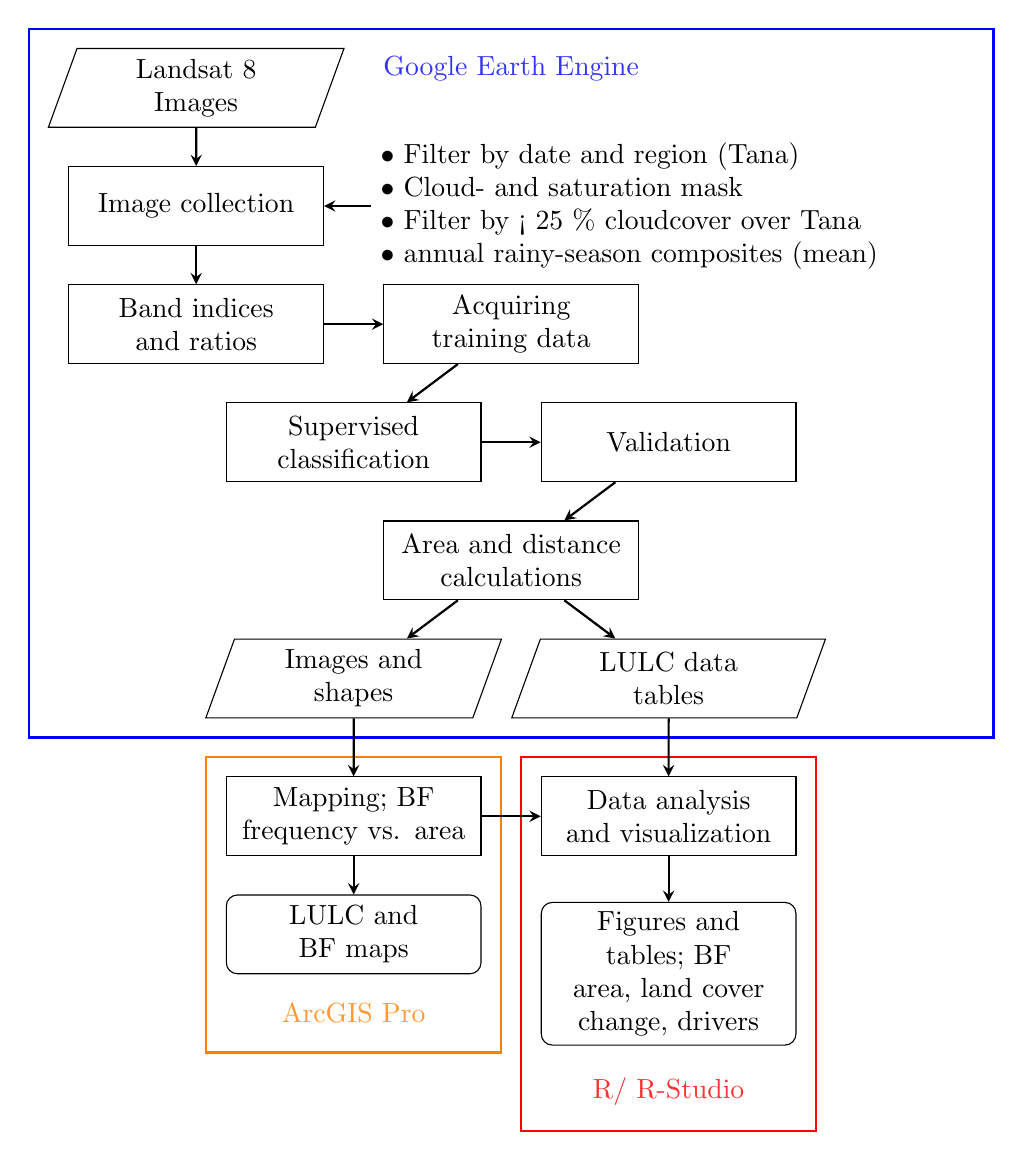
\begin{tikzpicture}[node distance=1.5cm]
%Gee
\node(GEEs)at(4cm,-3.75cm)[rectangle, minimum width = 12.25cm, minimum height=9cm, draw=blue!100, line width=.3mm]{};
\node(GEE)at (4cm,0.25cm)[color=blue!80]{Google Earth Engine};
\node(images)[io]{Landsat 8 Images};
\node(collection)[process, below of=images] {Image collection}; %at(1,8)
    \node[align=left](Det)[right of=collection, xshift=4cm]{
    $\bullet$ Filter by date and region (Tana)\\
	$\bullet$ Cloud- and saturation mask\\
	$\bullet$ Filter by < 25 \% cloudcover over Tana\\
	$\bullet$ annual rainy-season composites (mean)
	};
   % \node[fit={(D)(C)(F)(RS)}, inner sep=5pt] (box){};
\node(band)[process, below of=collection]{Band indices and ratios};
\node(train)[process, below of=band, xshift=4cm, yshift=1.5cm]{Acquiring training data};
\node(classi)[process, below of=train, xshift=-2cm]{Supervised classification};
\node(vali)[process, below of=classi, xshift=4cm, yshift=1.5cm]{Validation};
\node(calculations)[process, below of=vali, xshift=-2cm]{Area and distance calculations};
\node(gee)[io, below of=calculations, xshift=2cm]{LULC data tables};
\node(img)[io, below of=calculations, xshift=-2cm]{Images and shapes};

%R-Studio
\node(GEEs)at(6cm,-10.875cm)[rectangle, minimum width = 3.75cm, minimum height=4.75cm, draw=red!100, line width=.3mm]{};
\node(GEE)at (6cm,-12.75cm)[color=red!80]{R/ R-Studio};
\node(dataVisu)[process, below of=gee, yshift=-.25cm]{Data analysis and visualization};
%\node(reg)[process, below of=gee, xshift=4cm, yshift=1.5cm]{logistic regression};
\node(figtab)[startstop, below of=dataVisu, yshift=-.5cm]{Figures and tables; BF area, land cover change, drivers};


%ArcGIS
\node(GEEs)at(2cm,-10.375cm)[rectangle, minimum width = 3.75cm, minimum height=3.75cm, draw=orange!100, line width=.3mm]{};
\node(GEE)at (2cm,-11.75cm)[color=orange!80]{ArcGIS Pro};
\node(mapping)[process, below of=img, yshift=-.25cm]{Mapping; BF frequency vs. area};
%\node(freqtab)[io, right of=mapping, yshift=-.5cm, xshift=2cm, fill=orange!30]{backfill frequency table};
\node(maps)[startstop, below of=mapping]{LULC and BF maps};

%arrows
\draw[arrow](images)--(collection);
\draw[arrow](collection)--(band);
\draw[arrow](Det)--(collection);
\draw[arrow](band)--(train);
\draw[arrow](train)--(classi);
\draw[arrow](classi)--(vali);
\draw[arrow](vali)--(calculations);
    \draw[arrow](calculations)--(gee);
    \draw[arrow](calculations)--(img);
\draw[arrow](img)--(mapping);
    \draw[arrow](gee)--(dataVisu);
    %\draw[arrow](gee)--(reg);

    \draw[arrow](mapping)--(dataVisu);
    \draw[arrow](mapping)--(maps);
%\draw[arrow](freqtab)--(dataVisu);
\draw[arrow](dataVisu)--(figtab);
%\draw[arrow](reg)--(figtab);
\end{tikzpicture}
\caption{Methodical scheme. Parallelograms indicate input/ output data, rectangles indicate processes, and rounded rectangles indicate final results. The surrounding rectangles show, in which environment/ software processing took place.}
\label{fig:metsch}
\end{figure}

In addition to the satellite images used for the classification, various other external data sets were used. The training data (TD) created from \citet{Dupuy.2020a} for their land use and land cover classification was adopted and customized for the purposes of this project. further external data sets were used to define the study area, for the regression analysis, as image bands for the classification and for visualization purposes during the validation process (Table \ref{tab:extdata}).

%\newpage
%\begin{landscape}
\begin{table}[H]
    \centering
    \caption{Data that was acquired for the different analyses steps}
    \label{tab:extdata}
    \begin{tabular}{p{6.5cm}p{1cm}p{1cm}p{5cm}}
    \hline
      Name & Type & Res. & Source\\
      \hline
      Antananarivo - Madagascar - 2017, Land use reference spatial database & Vector & &  \cite{Defrise.19, Dupuy.2020a} \vspace{4pt}\\ 
      %\hline
     
      NASA SRTM Digital Elevation 30 m & Raster & 30 m & \cite{Farr.2007}\vspace{4pt}\\
      %\hline
      
      Roads (madagascar-latest-free) & Vector & & \cite{Geofabrik, OpenStreetMap}\vspace{4pt}\\
      %\hline
      
      Tsinghua FROM-GLC Year of Change to Impervious Surface  & Raster & 30 m & \cite{Gong.2020}\\
      \hline
       
       
    \end{tabular}
   
    \label{tab:my_label}
\end{table}
%\end{landscape}
\section{Study area}
The study region consists of the city of Antananarivo and its surroundings, also known as Greater Antananarivo. The climate in Antananarivo is warm and temperate, with a dry season in winter and a rainy season in summer. Typically, there can be seasonal floods due to the high precipitation in the rainy season, combined with topographical features. Almost a third of the cities' infrastructure is located in zones of high flood risk. (\cite{Ramiaramanana.2021}).  

As a study area for the analysis, the buffered boundaries of Greater Antananarivo were chosen, as also used by \citet{Dupuy.2020a}. Further, the area was restricted to the low plains, since the cultivation of rice and other irrigated crops mostly takes place there \parencite{Aubry.2012}. This was done by choosing areas within Greater Antananarivo at an elevation below 1260 m.a.s.l. and with a slope of less than 10°. These values were derived by visual interpretation of high resolution background images combined with the Digital Elevation Model (DEM). 
In a later step,  part of the remaining area to the North West of Antananarivo was discarded, due to suspected misclassifications. This was done along the watershed boundary in order to keep areas that are upstream from the city in the study area. Figure \ref{fig:studyarea} shows the final study area that was used, and the buffered outline of Greater Antananarivo.

\begin{figure}[H]
\includegraphics[width = 15cm]{figures/2_methods/Study_area.png}
\caption{Study area within Greater Antananarivo that was used for the supervised classification of satellite images. The study area was restricted to regions below 1260 m.a.s.l. and with a slope lower than 10°. The part to the North West of the city was discarded from the analyses due to suspected misclassifications.}
\label{fig:studyarea}
\end{figure}

\section{Satellite Images}

\subsection{Image collection}
This analysis uses Landsat 8-OLI  calibrated top-of-atmosphere reflectance satellite images (USGS Landsat 8 Collection 2 Tier 1 TOA Reflectance, courtesy of the U.S. Geological Survey), which have a spatial resolution of 30 m. The images of this collection are of the highest available quality and suitable for time-series analysis. They can be cloud- and saturation masked using the "QA\_PIXEL" and "QA\_RADSAT" bands. Landsat image collections can be accessed directly via GEE. 

Landsat remote sensing data was chosen because their image collections (combining different sensors) span over a long time series, which could enable an analysis over a longer period than for instance when using Sentinel data. Due to difficulties combining the data from different sensors (e.g. Landsat 5, 7 and 8) in the supervised classification, this project used Landsat 8 images exclusively, which are available since March 2013 until today. %Discussion point that it would be very interesting, to go further back with an analysis such as this. maybe by parametrizing a model specifically for backfills, maybe over various years training only for backfill vs not --> with more expert knowledge on different years and areas and training for every xth year in the time-series.

To create an image time-series on an annual basis, it was necessary to find at least one satellite image per year. These images should be from a similar time during the year to have similar atmospheric and vegetation conditions. Due to backfills occurring during the dry season, the images were collected outside this time-period. The idea being to capture most backfills that took place in one year by using satellite images outside the season when backfilling mainly takes place. Because these areas often stay barren for more than a year after being filled up, it is thus possible to capture the backfilling activity during one dry season. This means that if areas are backfilled and built over both in the same year, this would not be captured in the data. %discussion

Different approaches were tried for image acquisition. First, looking for single images in May or June after the rainy season. Subsequently, a different approach was chosen, by using image composites of all images taken during the rainy season. The advantage of using satellite images that were taken during, or after the rainy season is that vegetative surfaces are easier to distinguish from bare soil areas, compared to the dry season when fields are barren and can look quite similar to bare soil. The disadvantage is that images can often have a high percentage of cloud cover. This proved to be difficult especially when using single images, due to there often being high cloud cover over Antananarivo, which meant that in some cases the first cloud free image (over the city) in the year was from August or September, thus negating the idea of taking images outside the dry season. The problem of high cloud cover lead to the idea of using image-composites, meaning to combine the data of several images, taken during a certain time period.
This is the method that was adopted for this analysis:
All images originating in a certain time period where filtered for the percentage of cloud cover over the city (<25\%) and  masked for clouds, to exclude cloudy pixels. This was done using custom GEE algorithms. The remaining images for each year were then combined to one by taking the mean value per pixel. For the year 2013 there were not enough images (of a high enough quality) available during the chosen time period. For this reason, a single image from early June was chosen for this year (Table \ref{tab:imcom}).
\begin{table}[H]
    \centering
    \caption{Images and image composites (mean), that were later used for classification. All images are from the following collection, accissed in Google Earth Engine. Collection: USGS Landsat 8 Collection 2 Tier 1 TOA Reflectance, courtesy of the U.S. Geological Survey.}
    \label{tab:imcom}
    \begin{tabular}{ccc}
    \hline
        Composite & No. images & Acquisition date\\
    \hline
         2013 & 1 & 9 June 2013\\
         2014 & 6 & 1 October 2013 - 1 May 2014\\
         2015 & 6 & 1 October 2014 - 1 May 2015\\
         2016 & 7 & 1 October 2015 - 1 May 2016\\
         2017 & 3 & 1 October 2016 - 1 May 2017\\
         2018 & 4 & 1 October 2017 - 1 May 2018\\
         2019 & 8 & 1 October 2018 - 1 May 2019\\
         2020 & 3 & 1 October 2019 - 1 May 2020\\
         2021 & 4 & 1 October 2020 - 1 May 2021\\
         2022 & 3 & 1 October 2021 - 1 May 2022\\
         \hline
    \end{tabular}
    
    
\end{table}


\subsection{Pre-processing}
To prepare the images for the later analyses, they were clipped to fit the size of the study area (Figure \ref{fig:studyarea}), which contains most rice fields and other BGI. This has the advantage of excluding areas that are not directly relevant to the research question from the analysis, and of limiting the amount of data that is created and processed. As a further step, the band values of the images were used to calculate different indices, such as the Bare Soil Index (BSI), and ratios between different bands to use for the supervised classification. For this the Landsat 8 bands B2 (BLUE), B3 (GREEN), B4 (RED), B5 (NIR), B6 (SWIR1) and B7 (SWIR2) were used. Using indices and band ratios can be beneficial for classification purposes, because indices target specific land cover classes, and like band ratios, are less susceptible to shadowing effects and differences in lighting or in the atmosphere. This can yield higher accuracies, than the band values themselves \parencite{Bahadur.2009, Khatami.2016}. Spectral indices to use for the classification were chosen in order to better identify specific features like water bodies, vegetation, built-up surfaces and soil. Additionally, specific indices using the RED band were chosen, since this band was found to be helpful to visually distinguish bare soil areas. Band ratios were included to incorporate the visual and near infrared bands with simple calculations, from examples related to identifying geological features and soil moisture \parencite{Mwaniki.2015, NgoThi.2019}. Elevation and slope information is often found to be beneficial for classification purposes, and was thus also included \parencite{Bahadur.2009, Jones.1988, Franklin.1987}. The image bands (indices and ratios) that were used for the supervised classification are listed in Table \ref{tab:bandratios}.

%DEM has helpd increase classification accuracy 7-12
%Franklin 15 --> classification accuracy using landsat more accuracy with slope

\begin{rotatepage}
\begin{landscape}
\begin{table}
\caption{List of the bands that were added to the images for supervised classification. The indices and band ratios were calculated from Landsat 8 image bands. The band names in the formulas represent Landsat 8 bands. The Digital Elevation Model (DEM) is a USGS/ NASA product that was used as elevation band, and to calculate the slope band.}
\centering
\bgroup%start group
\def\arraystretch{2}%define cell height (for formula visibility)
\begin{tabular}{c c c}
  \hline
 Index/ Band ratio & Formula & References  \\ 
  \hline
Atmospherically Resistant Vegetation Index (ARVI) & \(\frac{(NIR-(2\cdot RED)+BLUE)}{(NIR+(2 \cdot RED)+BLUE}\) & \citet{Yuvaraj.2022, Kaufman.1992}\\
Bare Soil Index (BSI)& \(\frac{((RED+SWIR2)-(NIR+BLUE))}{((RED+SWIR2)+(NIR+BLUE))}\)& \citet{Diek.2017}\\
Color Index (CI) & \(\frac{(RED-GREEN)}{(RED+GREEN)}\) &\citet{Yuvaraj.2022}\\
Normalized Difference Built up Index (NDBI) & \(\frac{(SWIR1-NIR)}{(SWIR1+NIR)}\) & \citet{Zha.2003}\\
Normalized Difference Vegetation Index (NDVI)& \(\frac{(NIR-RED)}{(NIR+RED)}\) & \citet{Rouse.1973}\\
Normalized Difference Water Index (NDWI)& \(\frac{(GREEN-NIR)}{(GREEN+NIR)}\) & \citet{McFeeters.1996}\\
Redness Index (RI)& \(\frac{(RED^2)}{(GREEN^2)}\) & \citet{Yuvaraj.2022}\\
%Soil Composition Index (SCI)& (SWIR1-NIR)/(SWIR1+NIR) \cite{AlKhaier.2003}&\\
Ratio 4/3 & \(\frac{RED}{GREEN}\) & \citet{Mwaniki.2015}\\
Ratio 5/7 & \(\frac{NIR}{SWIR2}\) & \citet{NgoThi.2019}\\
Ratio 6/2 & \(\frac{SWIR1}{BLUE}\) & \citet{Mwaniki.2015}\\
Ratio 7/3 & \(\frac{SWIR2}{RED}\) & \citet{Mwaniki.2015}\\
Elevation [m] & & \citet{Farr.2007}\\
Slope [°]& & \citet{Farr.2007}\\

            
   \hline
\end{tabular}
\egroup%end group
\label{tab:bandratios}
\end{table}
\end{landscape}
\end{rotatepage}

\section{Training Data}\label{TD}
The training data (TD) that was used is based on reference data used by \citet{Dupuy.2020a} for their LULC classification of the Greater Antananarivo region in 2017. Their field survey was conducted during the 2017 rainy season. GPS waypoints were collected for the different LC classes and digitized to polygons using a VHSR Pleiades image (Very High Spatial Resolution, 0.5 m) to draw the boundaries of the corresponding landcover. Easily recognizable classes were digitized by photo interpretation \parencite{Dupuy.2020a}.

Since the goal of this analysis is to classify backfilled areas, polygons of known such areas needed to be digitized to get information on this landcover class. Next to 5 areas that were already known, a personal communication (section \ref{sect:BF-ts-validation}) with a professor from the University of Antananarivo (Prof. Dr. B. S. Ramamonjisoa), which was conducted to help in the validation process for areas classified as backfills, helped to establish a set of known areas that were backfilled, ending up with 23 known backfilled areas in 2017. Additionally, a landcover class named “Other bare soil”, containing undefined areas, that were often wrongly classified as backfills, was incorporated.

Using the composite image of the rainy season 2017 and the polygon reference data, the band values listed in table \ref{tab:bandratios} were combined with the landcover polygons using the “sampleRegions” function in GEE. This creates a point dataset with data on the landcover class and on the chosen band values for each point, which can then be used to train the supervised classification model.

The initial TD  was quite imbalanced (Figure \ref{fig:training:data}), possibly due to the image used for training being restricted to the study area (Figure \ref{fig:studyarea}), neglecting the TD polygons outside this compound. An imbalanced training data set can lead to over-fitting the supervised classification model for majority classes which have more training data available, like rice in this case. To avoid this, the TD obtained for the study area was downsamlped using random undersampling \parencite{KrishnaVeni.2011}. The partial downsampling of majority classes, without completely balancing the dataset can help the performance of rando forest classifications \parencite{Hasanin.2018}. For this, the data points of classes with more available data than backfills were randomly sampled to end up with a similar number of training points as backfills. The sampling was done using a uniform random distribution function in GEE (“randomColumn”, with distribution = ”uniform”), which assigns values between zero and one, which can then be used to filter points with a random number lower than, or equal to the fraction of $\frac{training~points~backfill}{training~points~other~class}$. The resulting downsampled TD  has a similar number of data points for ricefields, water bodies, Wetlands, industrial areas, and backfills, whereas the other classes have less training points. The classes fruit crop, forest, rainfed crop, other bare soil, and savannah all have below 100 training points in the data (Figure \ref{fig:training:data}). This was accepted, due to their low quantitative relevance in the study area, and because they are not of crucial importance considering the research question. Together, they made up for 5.5 \% of the downsampled training data. Since the class of backfill is of the highest importance for this analysis, possible under-representation of these classes was accepted. Another random column of the same sort as before was  added to the training data to later divide it into 10 different folds for validation (Section \ref{sect:classi-10fold}).

\begin{figure}[H]
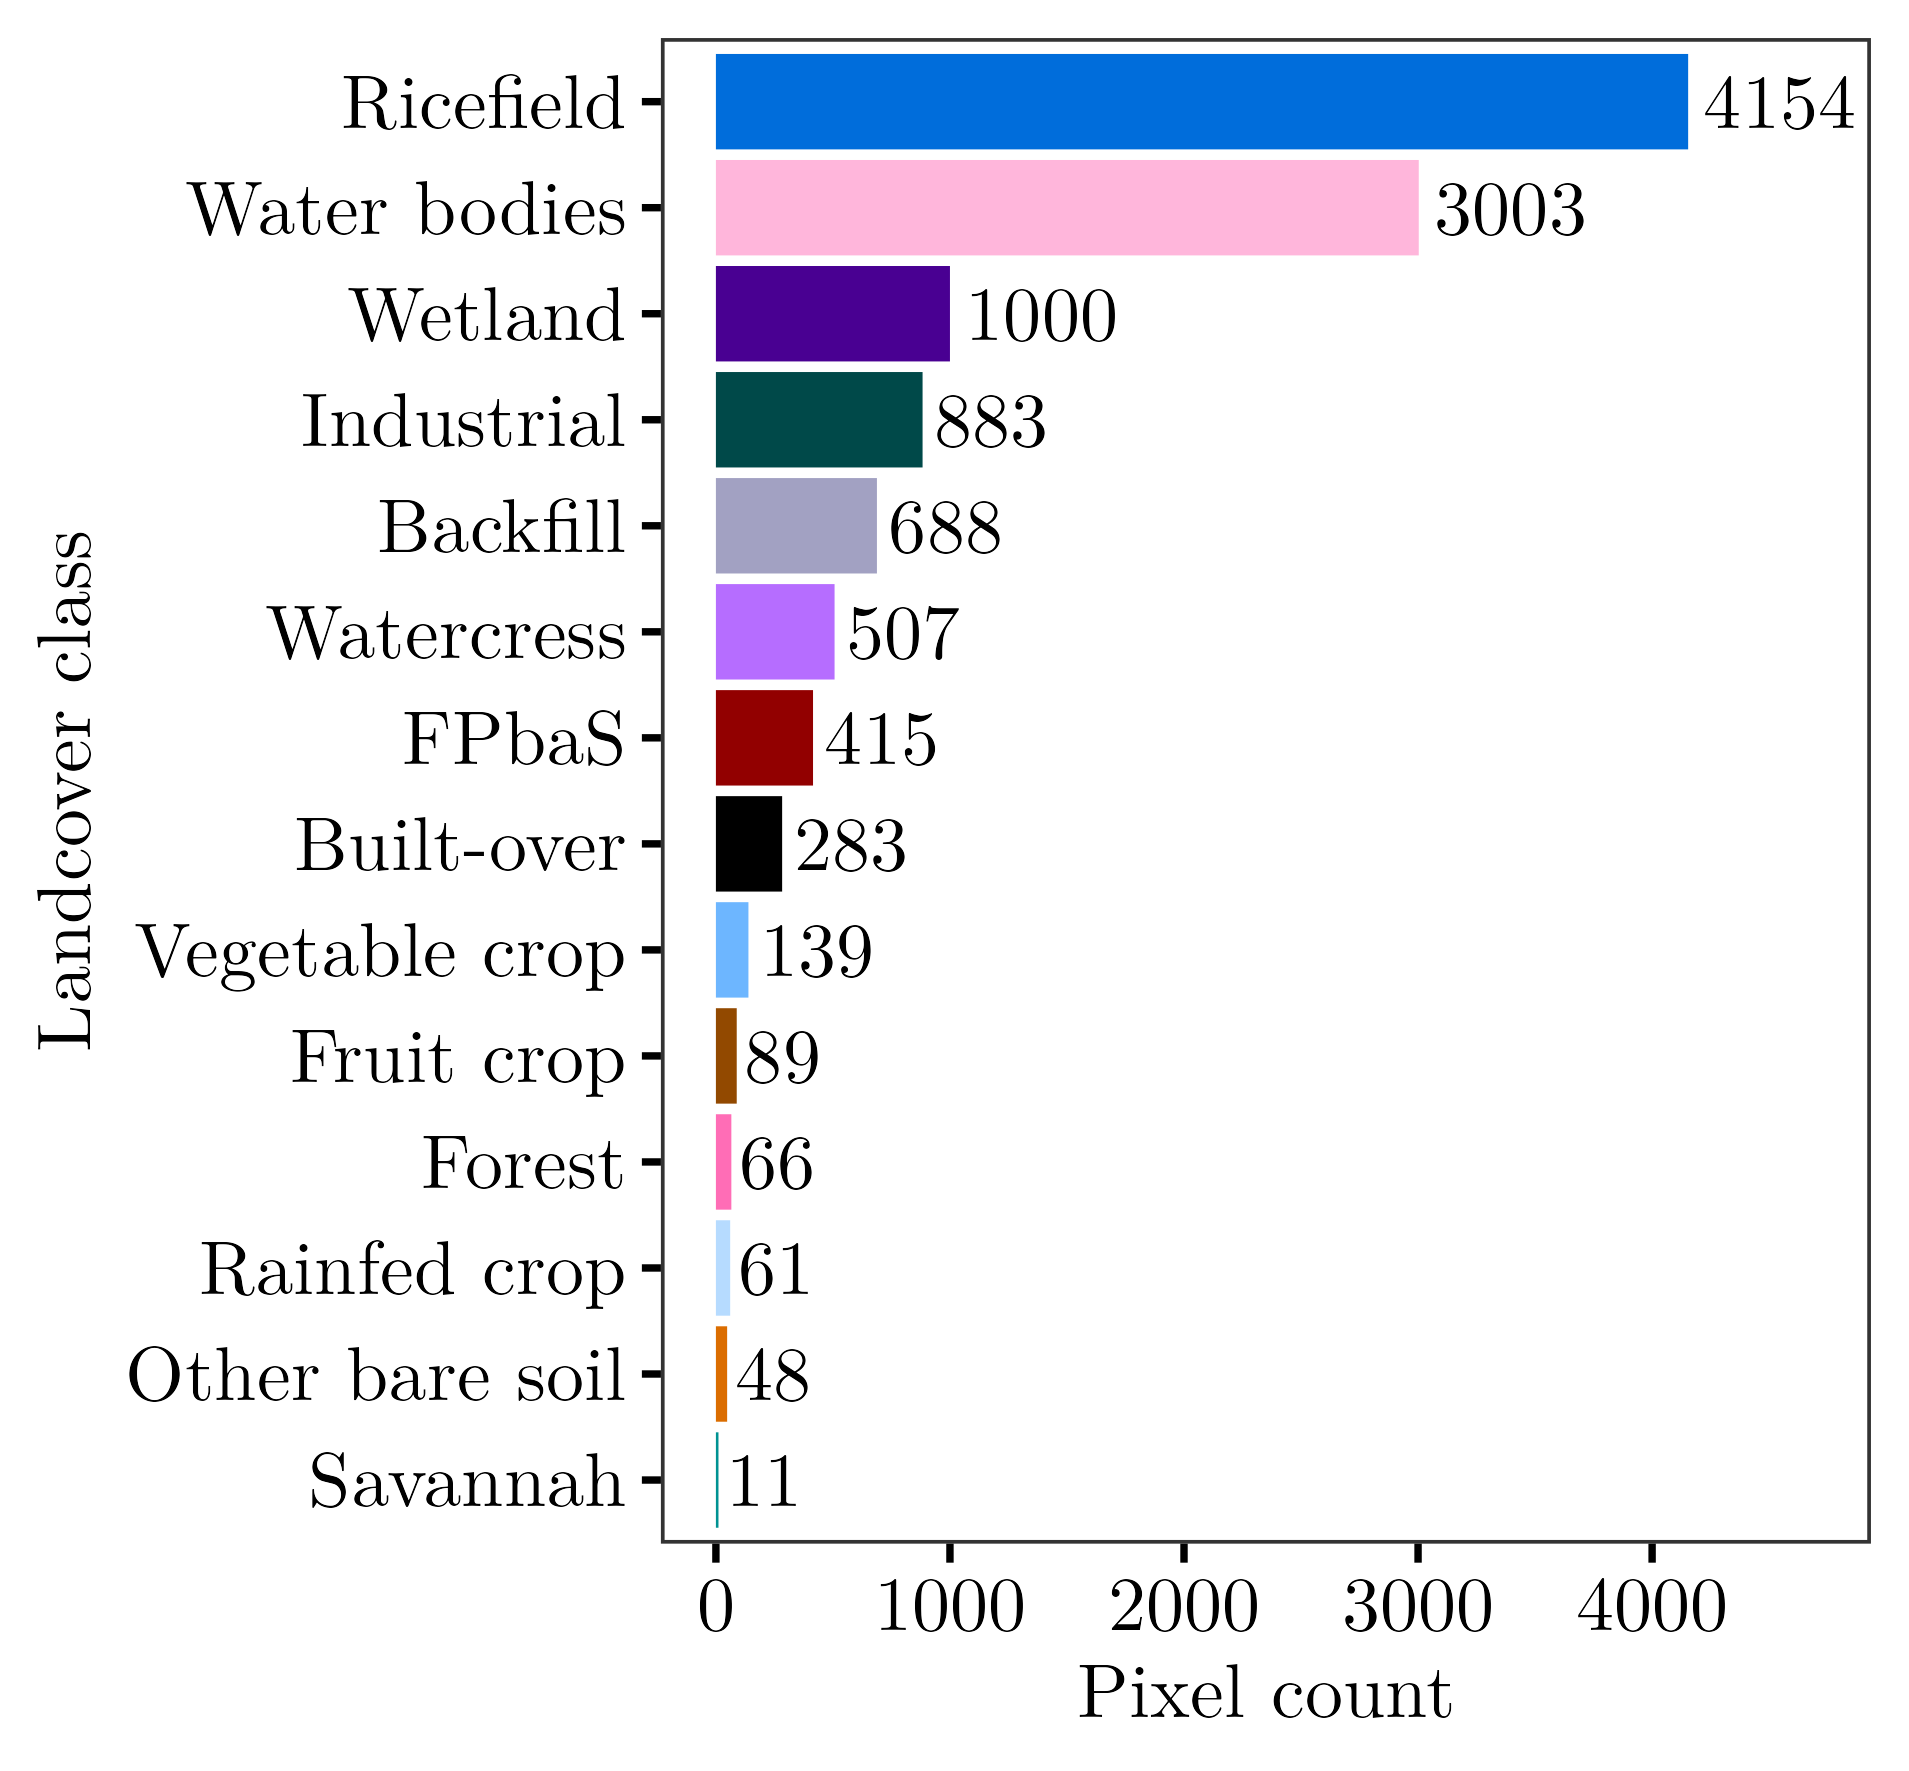
\includegraphics[width = 9.7 cm]{figures/2_methods/All training data.png}
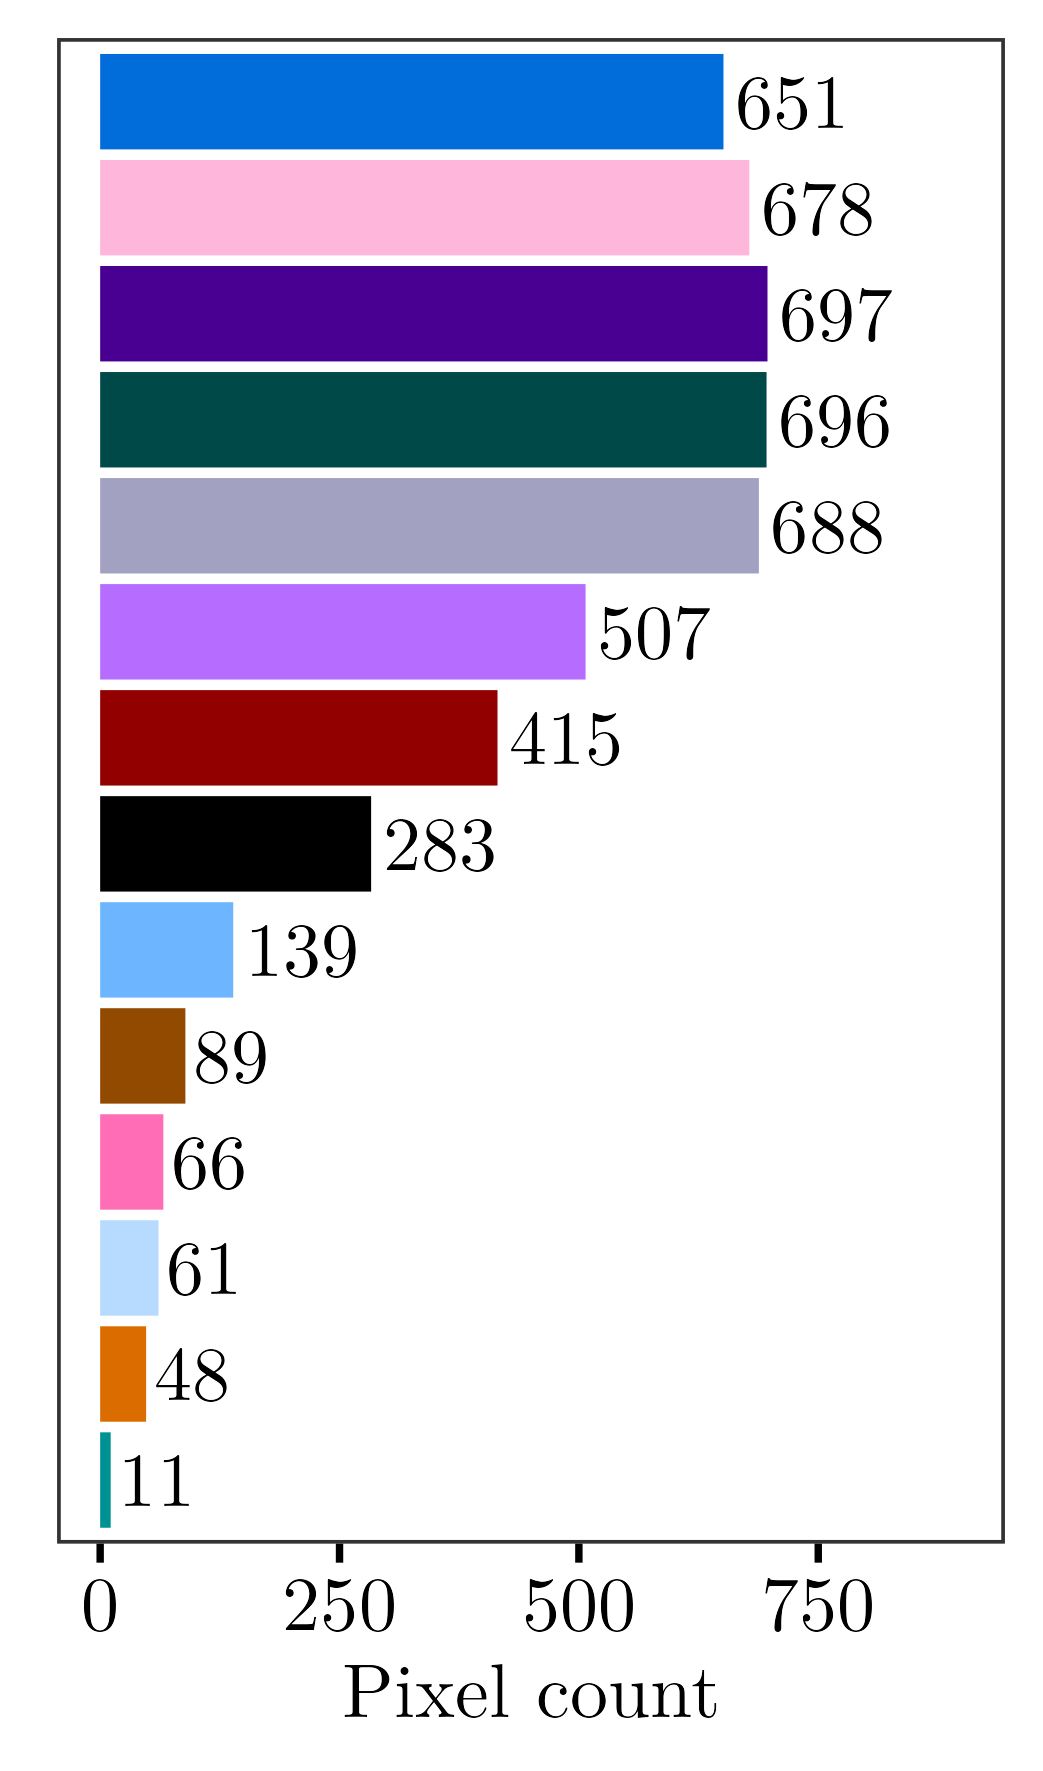
\includegraphics[width = 5.3 cm]{figures/2_methods/Subsampled training data to BF size.png}
\caption{Number of data points for each class used for training the supervised classification models. Due to the imbalanced nature of the initial data set (left), the data was randomly downsampled (right) to ensure that classes with a higher number of training points are in the same range as the backfill class.}
\label{fig:training:data}
\end{figure}

%--> cite Bruno: (J. Doe, personal communication, December 12, 2004)
\section{Supervised classification}
\subsection{Classification}
The supervised classification was initially run with three different classification models supported in GEE: The support vector machine classifier (SVM), the classification and regression trees classifier (CART), and the random forest classifier (RF). Due to a better performance (section \ref{sect:valid-results}), the latter was chosen for the analysis. It was run with default settings and a number of trees of 100. A higher number of trees can improve the measured accuracy of the random forest classification. \citet{Probst.2017} found that in the N datasets they analyzed, the biggest gain in performance was reached within the first 250 trees, after which the value most of the time did not improve anymore. For the 29 datasets they tested, \citet{Oshiro.2012} describe no considerable increase in mean and median AUC performance after more than 64 trees and suggest a range between 64 and 128. Choosing a too high number of trees can potentially also lead to over-fitting the model, thus it is suggested to use a high and computationally feasible number of trees (\cite{Probst.2017, Oshiro.2012}). To ensure the reproducibility of different runs, the model was run with a random seed. The training data obtained with the LULC polygons and the median image of the year 2017 was used to train the supervised classification model that was then used to classify all 10 images/composites of the study area. 

\subsection{Validation}\label{sect:classi-10fold}
The classification models were validated for the year 2017 using a 10-fold cross-validation approach \parencite{Rodriguez.2010}. \citet{Wong.2020} state, that it can be beneficial in k-fold validation to use only one run with 10 randomly chosen folds. This is the method that was employed here, using 10 folds containing 508 Data points on average (SD= 16.5).
The training data (Figure \ref{fig:training:data}, right) was randomly split into 10 evenly sized folds using uniformly distributed random numbers between zero and one to filter it by intervals of 0.1. Then, a function was created to run ten classifications, leaving each fold out once. Each of the classification runs was validated separately, using the fold that was left out as test data to create an error matrix and calculate the overall accuracy and kappa coefficient. The mean values of overall accuracy and kappa coefficient were then used to estimate the overall accuracy of each classification model.
%maybe come back to only using 2018 --> 2017 for the regression analyses, knowing that tha classification for 2017 is at least decent

A conversion rate of BGI being backfilled in the study area was established by plotting the classification in the previous year for all the yearly backfill increase layers per frequency. The frequencies were combined for the classes ricefield, watercress, wetland, vegetable crop and water bodies, which are all considered as BGI.

\section{Backfill area increase}
\subsection{Time-series}
A time-series of newly backfilled areas per year was created using the ten classified images. Every image was first filtered by landcover value to only show backfill areas. The collection of ten images enabled to create 9 layers of backfill area increase per year. This was done by masking areas classified backfills in one year with the backfills in the years before, resulting in a yearly increase. This grid layer of yearly backfill increase was converted to a polygon, enabling the calculation of its area.

\subsection{Backfill size distribution}
The increase data was further processed to find the frequency of different sizes of backfilled areas. In Arc GIS Pro, the backfill increase layers were split into separate polygons for each area of adjacent backfill pixels. To ensure that also diagonally neighboring pixels and areas at a distance of one pixel from one another were grouped for the calculation of the area of a single backfill, the polygons were spatially joined with a buffer of 30 m. Of these layers, the area per contiguous shape was calculated, indicating the area in m$^2$ of that specific backfill. The resulting table, containing data for all years combined, was exported to create a histogram plot showing the frequency distribution per size of a backfill area. 

\subsection{Validation}\label{sect:BF-ts-validation}
To establish data on backfill areas, that could later be used to validate the time series, we conducted two extensive interviews with Prof. Dr. B. S. Ramamonjisoa of the University of Antananarivo: School of Agronomy. The interviews were designed to produce binary data on suspected backfilled areas, with the goal to gain as much data as possible in the available time. We used maps with the areas classified as backfills, resulting from the first supervised classification attempts, as a basis. From the images of the years 2013, 2017 and 2021 areas  that the classification identified as backfills were chosen to discuss (Table \ref{tab:backfill_Bruno}, p. \pageref{tab:backfill_Bruno}). Close attention was paid, to choose potential backfills distributed over the whole study area and incorporate  big as well as small areas. For each of the years, a polygon layer containing all the areas to discuss and a background image as visual reference was prepared in ArcGIS Pro. For the years 2017 and 2021, background Maps\footnote{10 m, Planet and NICFI Basemaps for Tropical Forest Monitoring - Tropical Africa, Planet Team (2017). Planet Application Program Interface: In Space for Life on Earth. San Francisco, CA. https://api.planet.com; accessed in GEE} 
in a higher resolution  were available and thus used for identification. For the year 2021 also the background imagery of ArcGIS PRO\footnote{Esri, Maxar, Earthstar Geographics, and the GIS User Community} 
was useful, to see if the 2021 areas were still backfills to date, or already built over. For all of these years also the Landsat 8 image (composite) used for classification was available. Using these means, we discussed each of the areas shortly, going through them quite fast. The main information collected being if the area could be confirmed as backfill (1), if it could be confirmed as not being a backfill (0) or if it was unclear(2). %Discussion: i think the 2013 values might be worse due to worse background image and more unsures?
Each separate area was assessed using the following main criteria:
\begin{itemize}
\item Geographical location
\item Memory/ knowledge of the area
\item Looking at the reference images to see the area and its elevation and surroundings
\end{itemize}


The resulting information was used twofold. First to have more elaborate data on backfills for the year 2017 to help train the model, and secondly to get an idea of the accuracy of the time-series by assessing it separately for each of these three years, creating error matrices and calculating accuracy coefficients.

\begin{table}[H]
    \centering
     \caption{List of the areas that were looked at to identify backfills in three years. 0 = not a backfill; 1 = backfill; 2 = unsure. The total lists the number of areas that could be used for training and validation (0 and 1).}
    \label{tab:backfill_Bruno}
    \begin{tabular}{cccc}
    & \multicolumn{3}{c}{Year}\\
        \hline
       Validation code & 2013 & 2017 & 2021\\
        \hline
        0 &  10 & 15 & 14\\
        1 & 25 & 23 & 35\\
        2 & 18 & 18 & 6\\
        \hline
        Total & 35 & 38 & 49\\
        \hline\\
    \end{tabular}
\end{table}

To validate backfilled areas in these three years, simple error matrices were established after the classifications. These then allowed the calculation of overall accuracy, Cohen's Kappa, producer's- and user's accuracy. The overall accuracy is calculated by dividing the total of correctly classified pixels by the total number of pixels that were classified.  \parencite{Congalton.1991}. For the producer's accuracy,  ,,the total number of correct pixels in a category is divided by the total number of pixels of that category as derived from the reference data'' (\cite{Congalton.1991}, p.36), and for the user's accuracy ,,the total number of correct pixels in a category is divided by the total number of pixels that were classified in that category'' (\cite{Congalton.1991} p.37). The Cohen's kappa is a coefficient of agreement for nominal scales, such as error matrices, described by \citet{Cohen.1960}. It is a measure of agreement, which excludes agreement by mere chance.

\newpage
\section{Drivers of Backfilling} 
Using two auxiliary datasets of roads and impervious surfaces as well as the other classes established through the supervised classification, we tried to find out, which variables can be important for the appearance and distribution of new backfills. Distance rasters created in GEE, as used by \citet{Floreano.2021} to investigate driver variables, were created for all these datasets. They were combined with the backfill increase and layers of the classified images in GEE, thus giving information on the landcover or backfill increase in a year and the distances to the chosen variables in the previous year, as well as the classification in the previous year. Further processing in R the previous year classification was used to create dummy variables signaling the previous year classification for a specific pixel and class in binary. For instance, a backfill that had been classified as rice field a year before would have a value of one, whereas if it was classified differently it would have a value of zero.  

The data on roads was sourced from OpenStreetMap \parencite{Geofabrik}. For the analyses, only primary and secondary roads were chosen for simplicity. Since the regression would be run over several years it was therefore still feasible to try and identify roads that were newly built over the time-series, to exclude them in the years before they had been built. This was important, as to not create a bias due to newly built roads that were identified as backfills.

To investigate the influence of the chosen independent variables on backfills, a binary logistic regression model was employed \parencite{Peng.2002, Manning.2007}. The logistic regression model should compare the binary state of an area being backfilled in the next year or not, with the distribution of the continuous and categorical predictor variables. Before running the model, the classes backfill, built-over, and industrial were excluded from the control dataset to only compare newly appeared backfills with other landcover classes, and assuming that already urban/ built-up areas will not be relevant since backfills are not expected to occur there. The control dataset was substantially larger than the number of data points on newly occurred backfills, and was thus randomly sampled to the same size before the regression. The logistic regression was conducted in R, using the ``glm'' function. The performance of the logistic regression model was assessed with Mc Faddens pseudo R$^2$.


\newpage
\chapter{Results}
\section{Supervised classification}\label{chap:supervised_classi}
\iffalse 
maps illustrating:

1 growth 2017 good map showing increase vs existing BF

2 distribution

5 --> these points might prompt to say in discussion, that the mean value is probably more valuable than yearly growth comparison and thus also calculate the rate of BGI being backfilled with a "mean year" having taken mean increase and the fraction of mean class distribution that was backfilled the year after.

-->the backfill masking was done with all years. if i still have time at some point i should to the same for previous year bf in regression. and otherwise mention this!

-->it might have been beneficial, to only train the model on "new" backfill!

6 --> the frequent misclassification between rice and wetlands or water is a good reason to consider all of these combind as BGI in the later analyses, especially for the rate. maybe also the image 2016 can be taken to argue that i should only do the regression or 2018 --> 17, which i think makes more and more sense.
\fi

\subsection{Validation}
Of the three supervised classification methods that were compared, the Random Forest classification performed the best for the year 2017, for which the training data was used for 10-fold cross-validation. Therefore, this model was chosen for usage in the further analysis. The overall accuracy of the Random forest classification for this year, using the downsampled training dataset, was 0.84 and the Cohen's Kappa value was 0.82 (Table \ref{tab:10Fcv_res}).

\begin{table}[ht]
\centering
\caption{Comparison of the overall accuracy and Cohen's Kappa for three supervised classification models for the classification of the 2017 image composite. Next to the accuracy estimates, the standard deviation is given, since the estimates are the mean of 10 test runs during the cross-validation.} 
\begin{tabular}{ccccc}
  \hline
 Classifier & Accuracy & $\sigma Accuracy$ & Kappa & $\sigma Kappa$ \\ 
  \hline
\textbf{Random Forest} &\textbf{ 0.84} & 0.02 &\textbf{ 0.82} & 0.02 \\
Classification and Regression Trees & 0.78 & 0.02 & 0.75 & 0.03 \\ 
Support Vector Machine & 0.76 & 0.02 & 0.73 & 0.02 \\ 
   \hline
\end{tabular}
\label{tab:10Fcv_res}
\end{table}

\subsection{Classification}\label{chap:classifiedmaps}
Two of the classified images, for the years 2017 and 2016, that were used for the further analysis, are shown below (Figure \ref{fig:cls17} and Figure \ref{fig:cls16}). The comparison illustrates the differences in classification between years that occurred in some cases. Some classified LULC types like built-up or industrial[..] are more consistent between images of different years than others, for instance rice field or wetland, which overlap strongly, when comparing the images of 2016 and 2017. These two images also show the differences between backfill classifications in different years. 2016 shows mainly patches of backfilled areas, whereas in 2017 next to patches of single areas also two roads are visible: The ``Boulevard de la Francophonie'' (North West of the city) and the ``Lalana Tsarasaotra-Ivato'' (North of the city) that had been newly backfilled or built, were also classified as backfills (Figure \ref{fig:Rt_franco}, p. \pageref{fig:Rt_franco}). For the Bvd. de la Francophonie that was probably already finished on the date of the satellite images used for classification, it seems like the backfilled soil surrounding the road's surface was classified as backfill. Compared to other areas, that often stayed barren over several years or even the whole time series, roads were observed to be backfilled and then built over quite fast, often over the course of one year. The classified images of all other years are shown in the Appendix.

%the bvd f shows error due to scale in the end for interpretation still valid, since 
% the road already being finished might well be the reason, why it is so pixelated (classified bf)
\begin{figure}
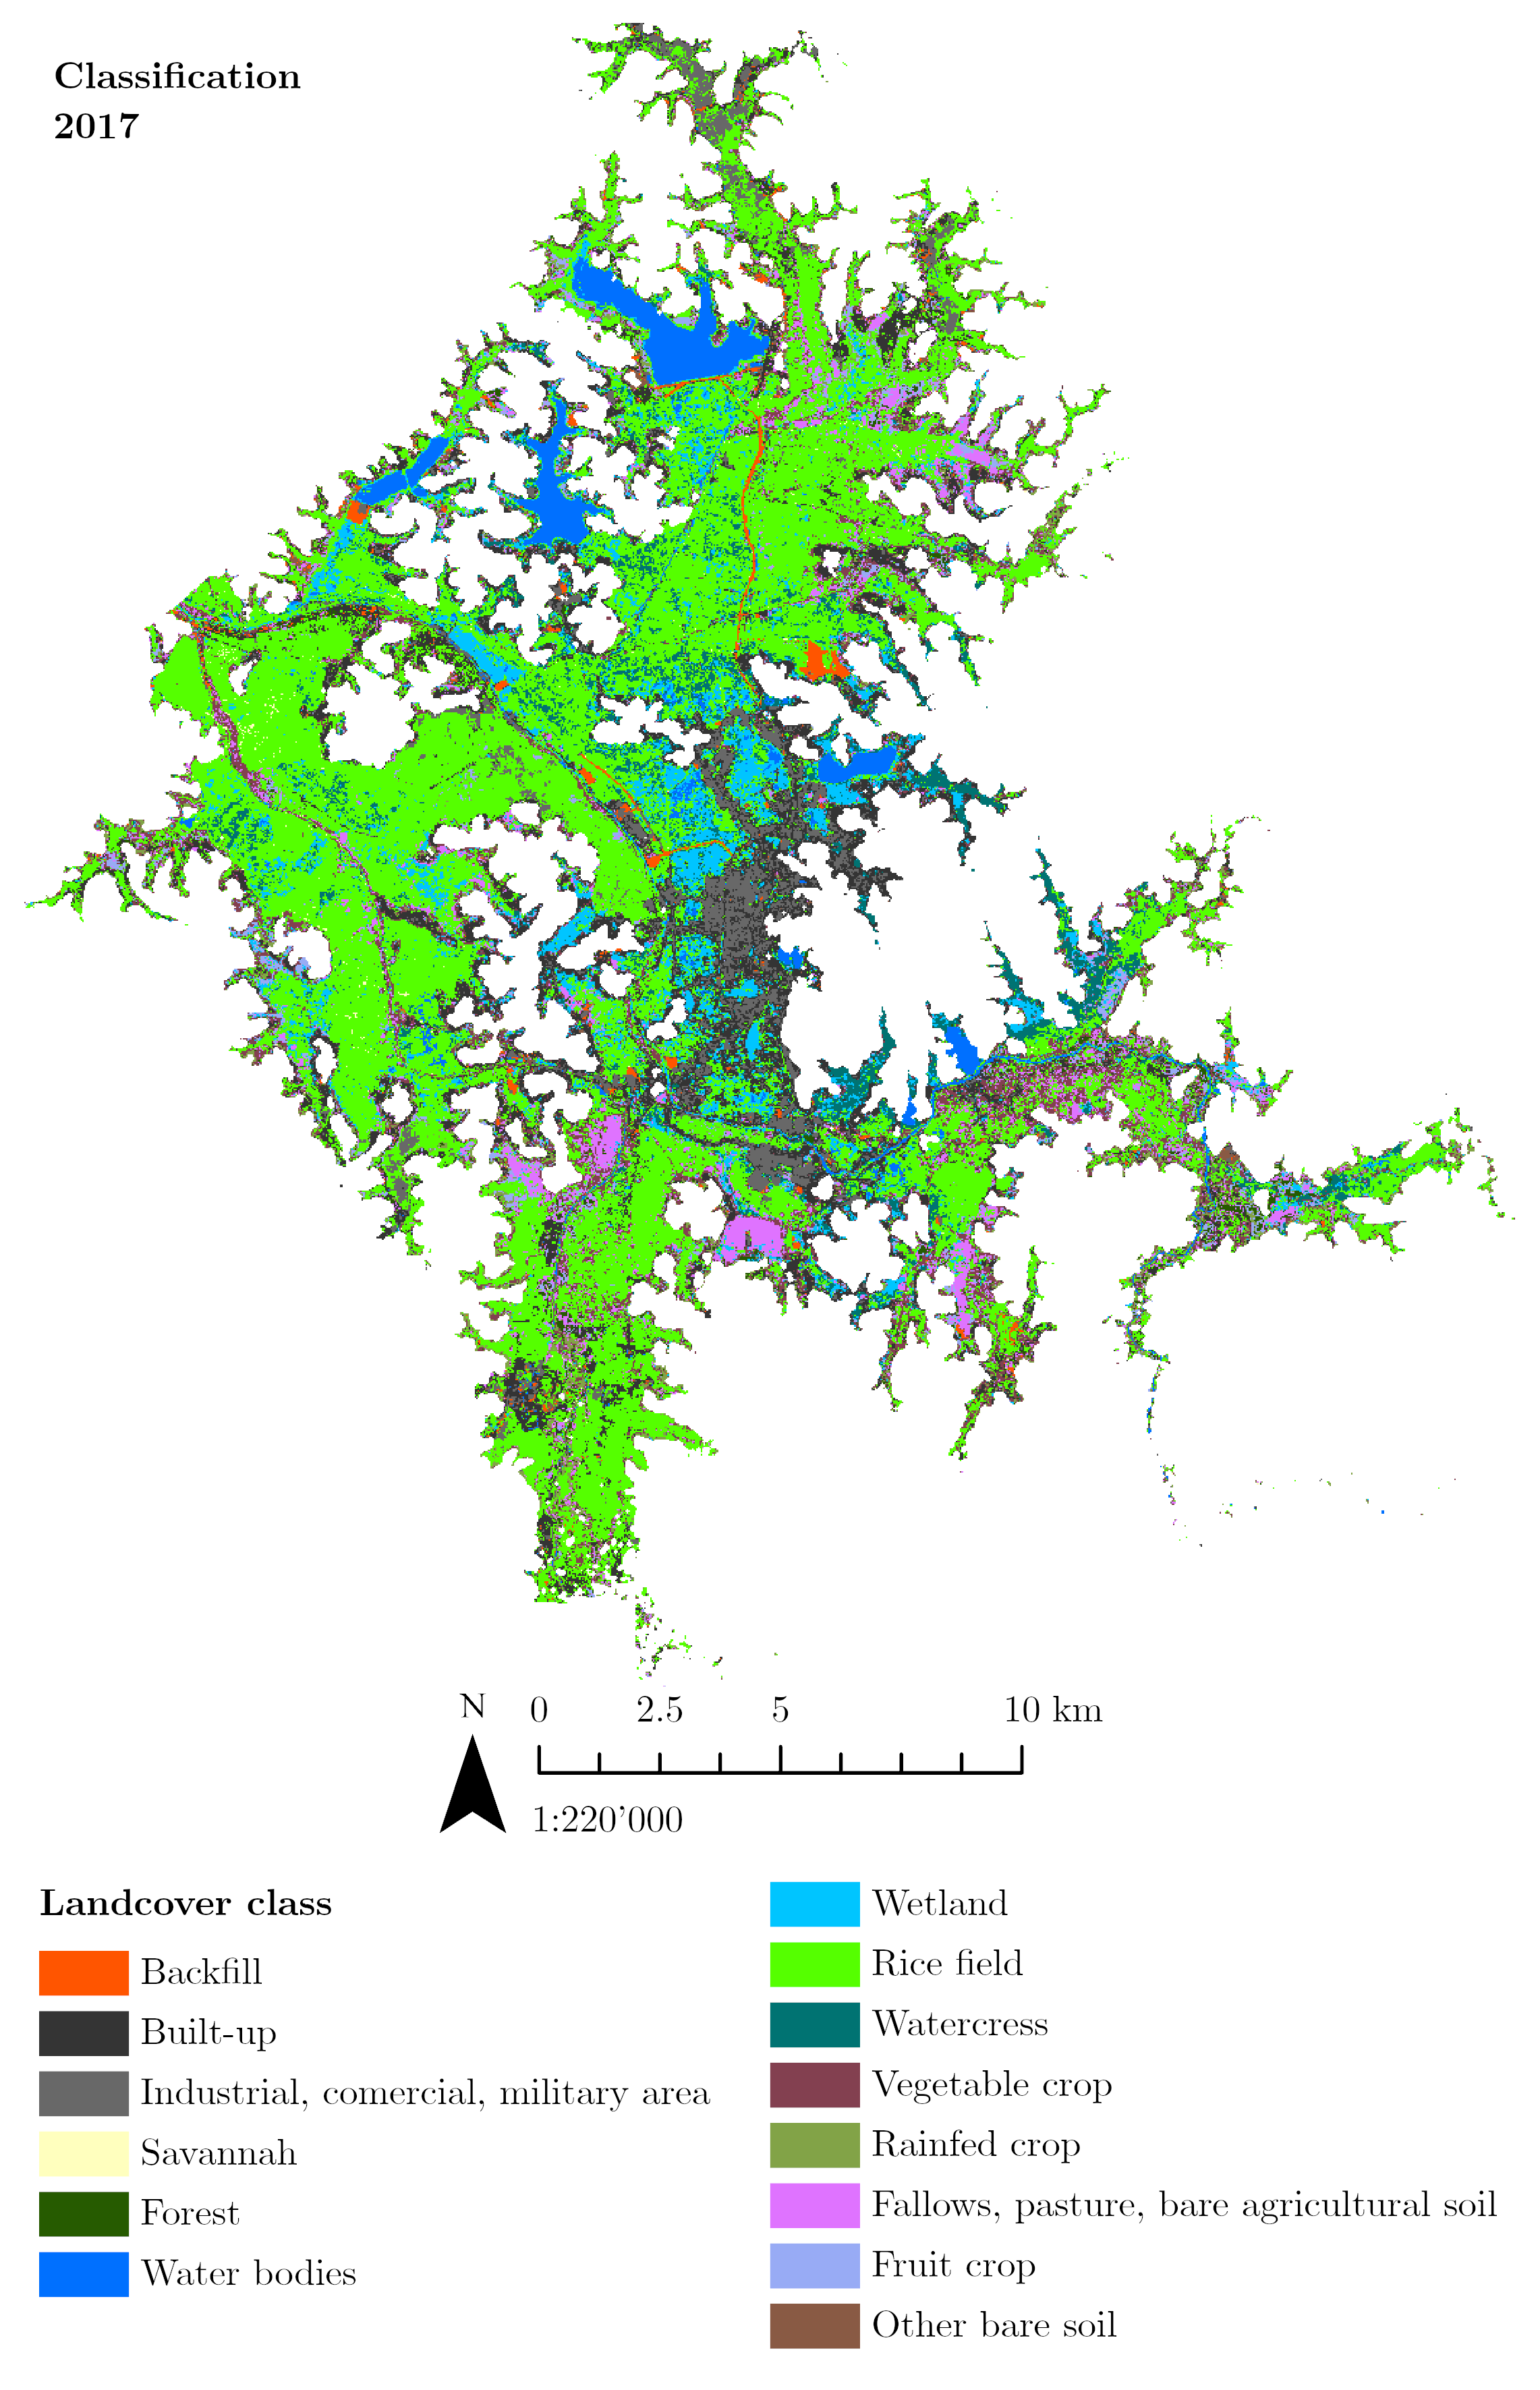
\includegraphics{figures/3_results/classi2017.png}
\caption{Classified image resulting from the 2017 classification.}
\label{fig:cls17}
\end{figure}

\begin{figure}
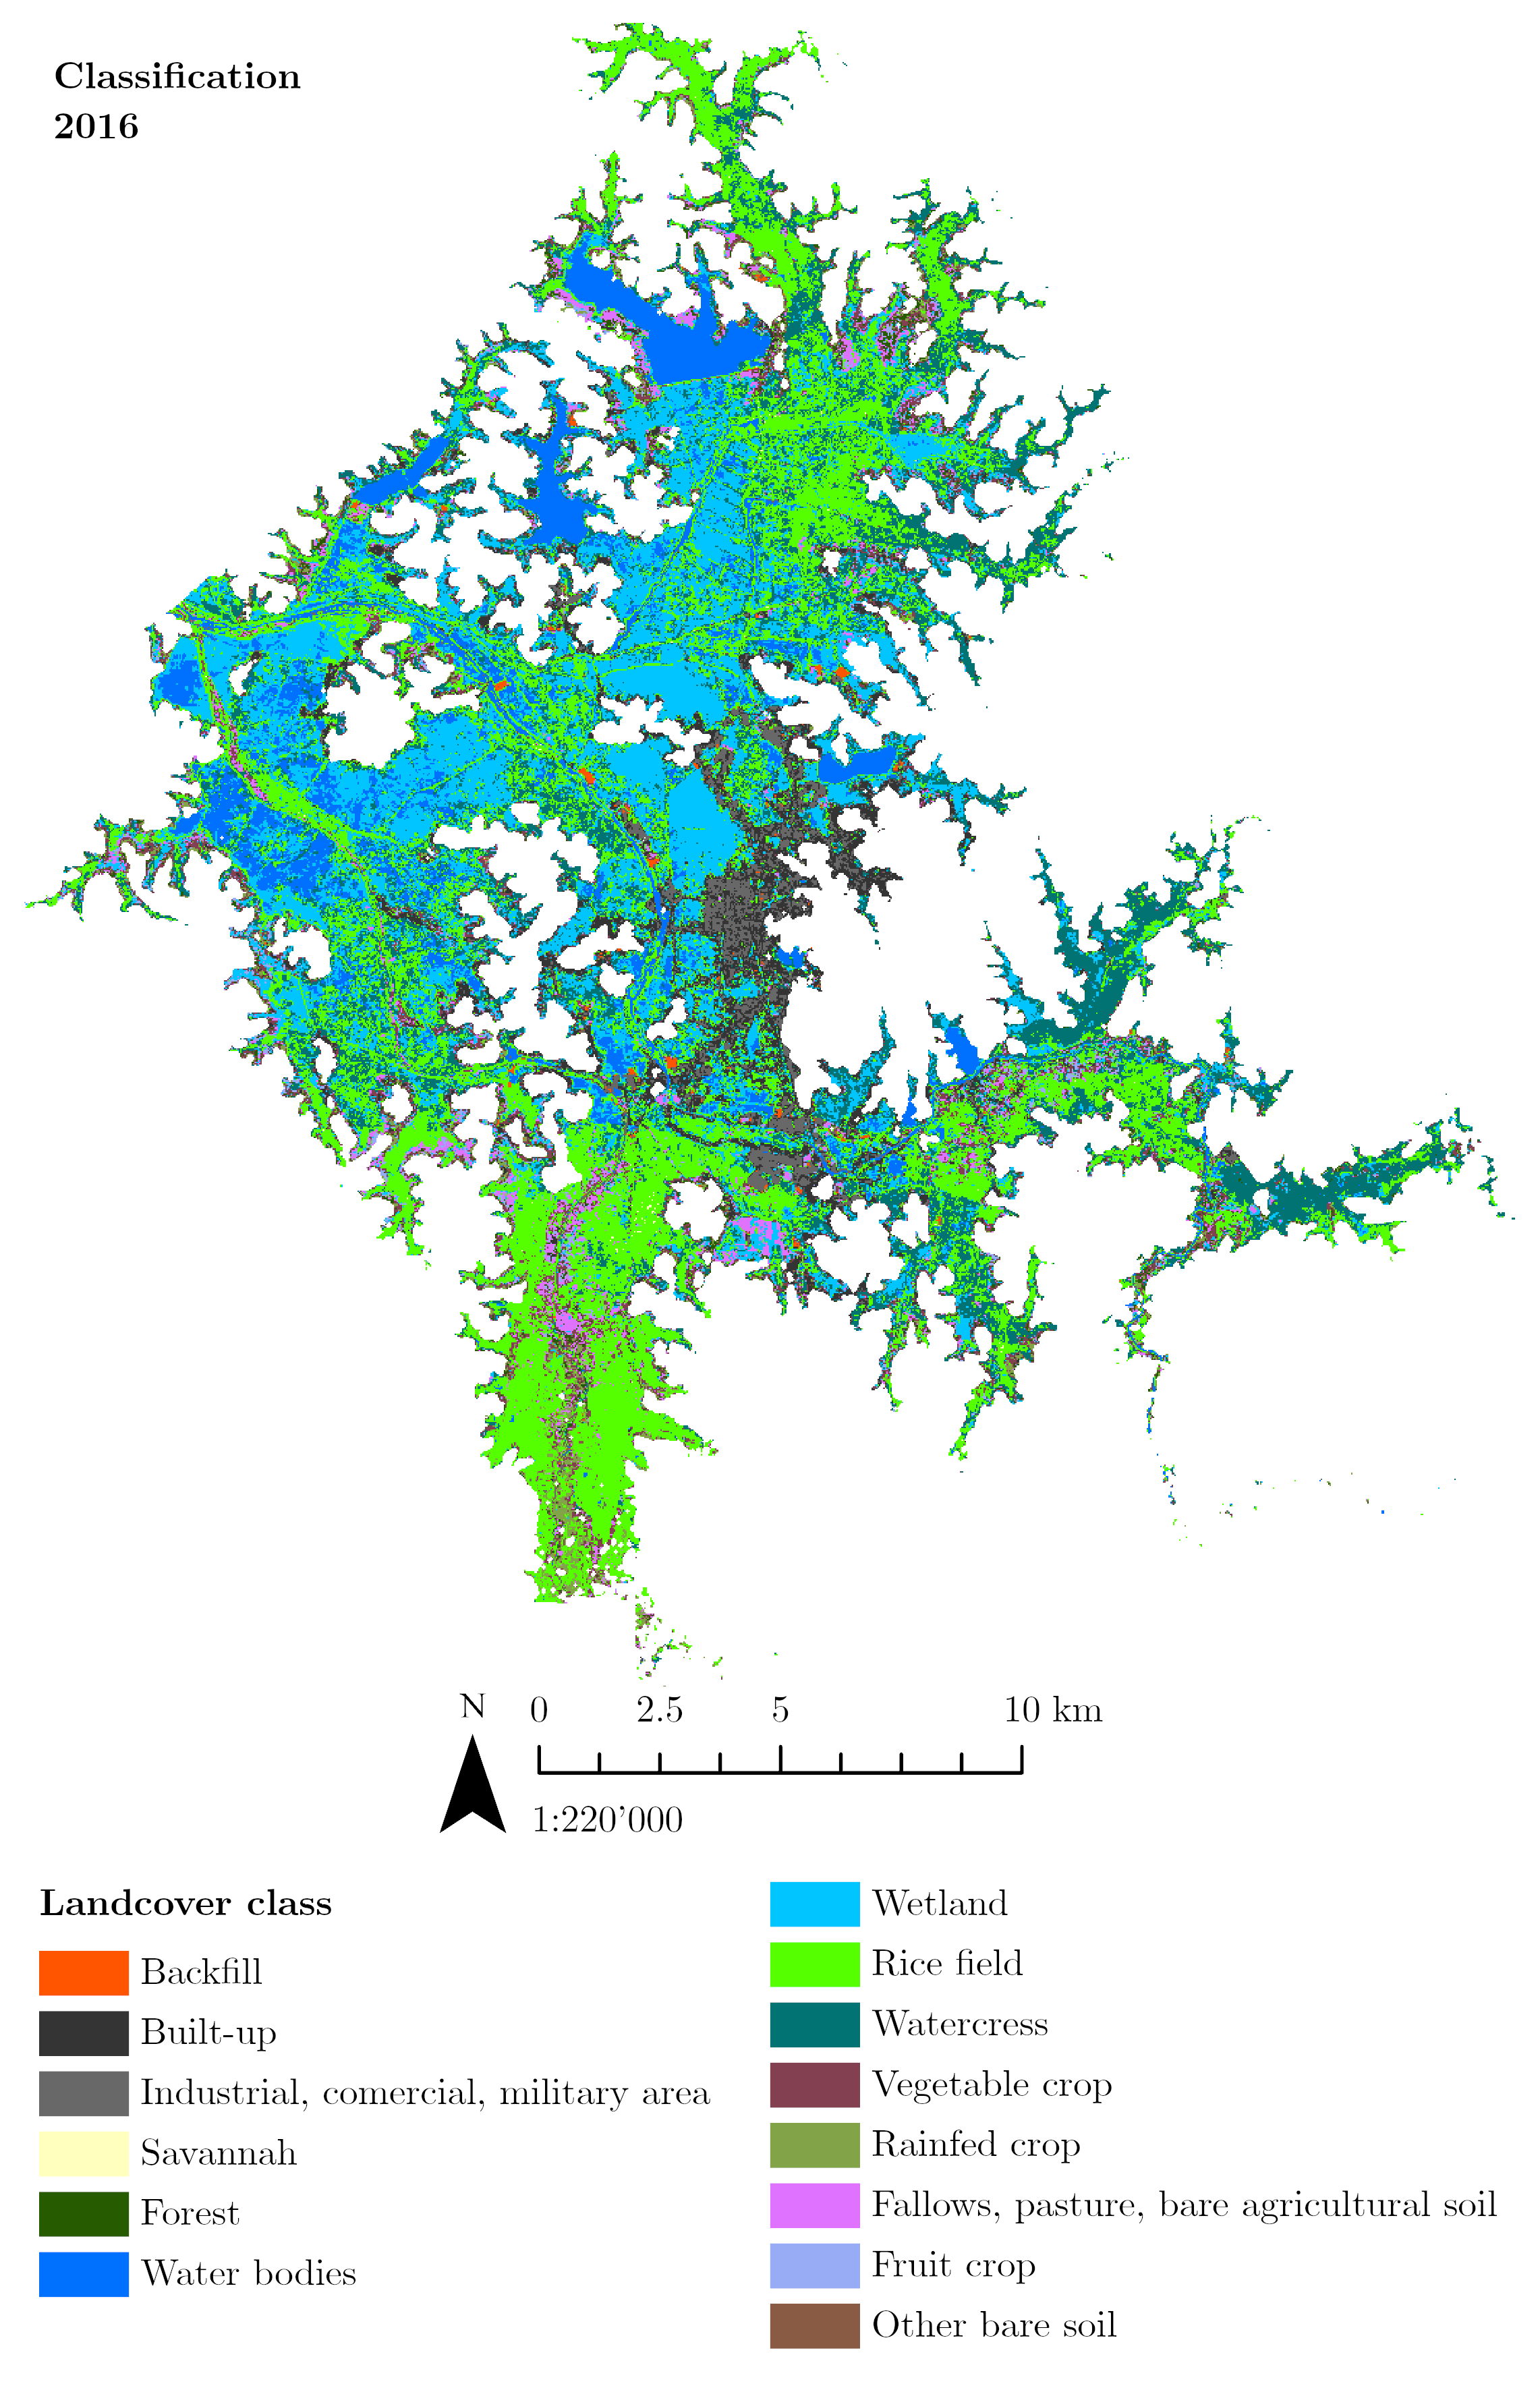
\includegraphics{figures/3_results/classi2016.png}
\caption{Classified image resulting from the 2016 classification.}
\label{fig:cls16}
\end{figure}

\begin{figure}[H]
    \centering
    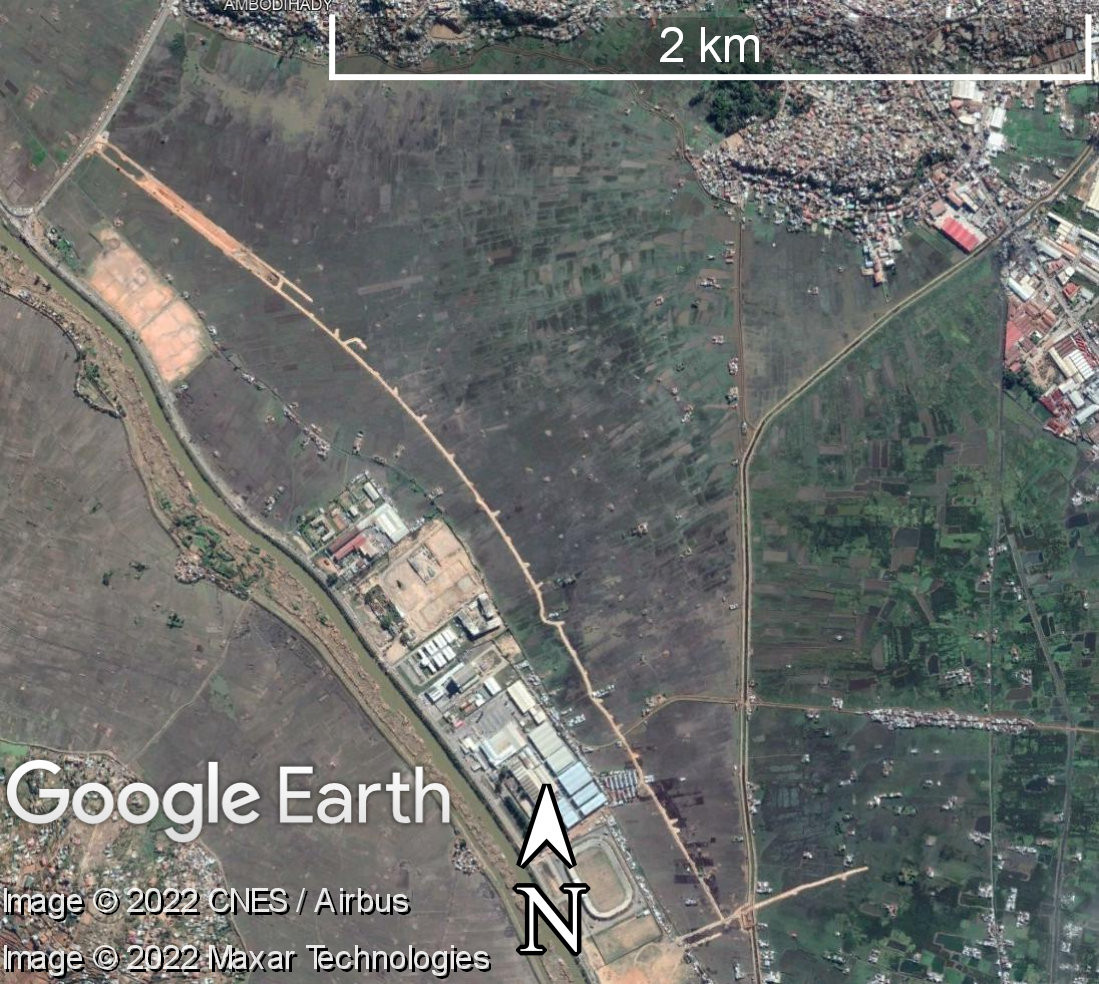
\includegraphics[width = 7.25cm]{figures/3_results/Rt_Francophonie_062016.jpg} \hspace{.25cm}
    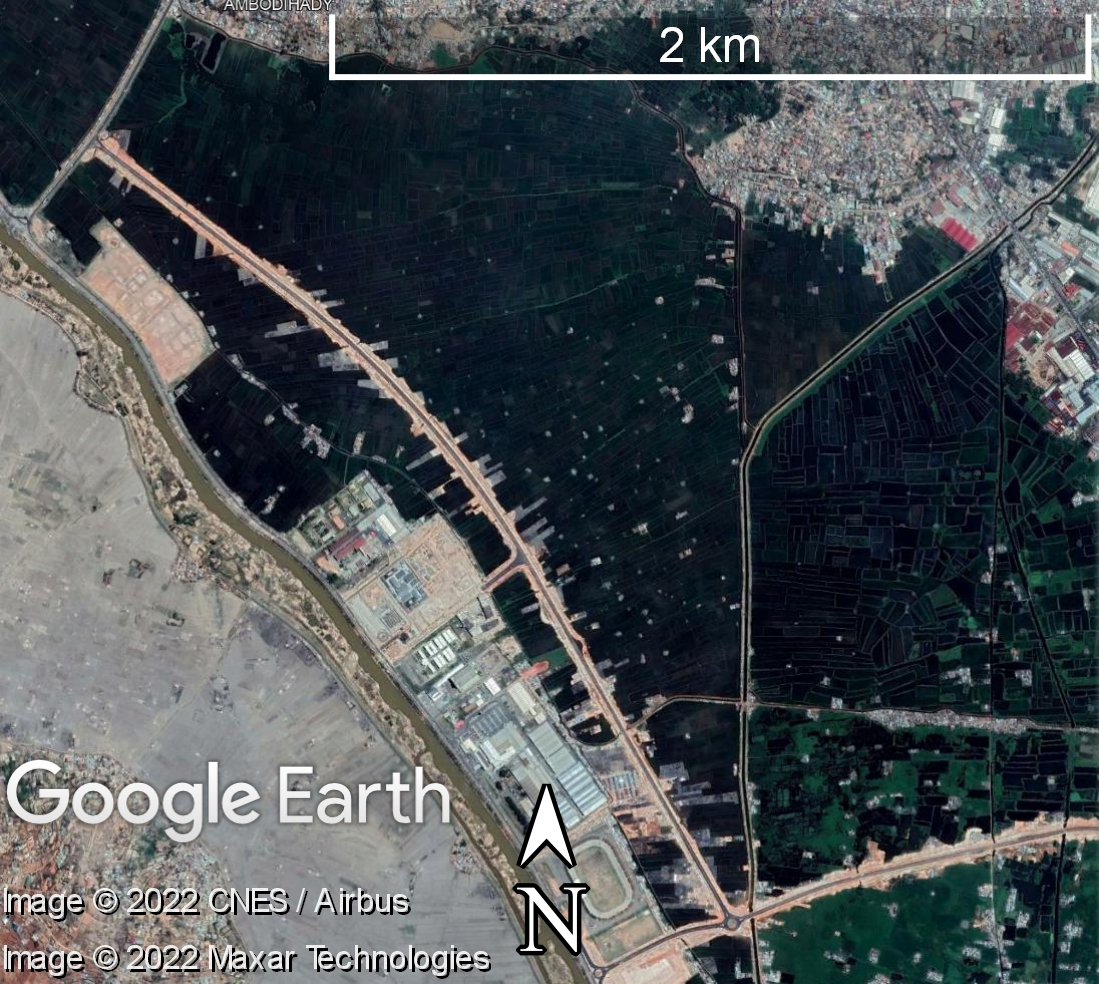
\includegraphics[width = 7.25cm]{figures/3_results/Rt_Francophonie_102016.jpg}
    \caption{Satellite images showing the development of the building/ backfilling of a road (Boulevard de la Francophonie). The image on the left is dated to June 2016, and the one on the right to October 2016. In contrast to other backfilled areas, which often stay barren over many years, roads seem to be backfilled and built quite fast (within one year).}
    \label{fig:Rt_franco}
\end{figure}

\section{Backfill area increase}\label{sect:valid-results}

\subsection{Validation}
The backfill time series was separately validated for two years other than 2017 of which the data was used for training the model and was assessed with cross-validation. To cover the range of the time-series, backfill classifications were validated for the years 2013 and 2021, creating simple error matrices representing ground truth resulting from expert interviews and the classification result of the same areas (Table \ref{tab:BFerrmat}, p. \pageref{tab:BFerrmat}). From these error matrices, the overall accuracy and Cohen's Kappa were calculated (Table \ref{tab:BFAcc}, p. \pageref{tab:BFAcc}).
For the training year of 2017 all backfill classifications align with the training data. This is mirrored by the accuracy estimates of one,  showing a high resubstitution accuracy, meaning the level of accuracy when classifying the data a model was trained with.
The mean overall accuracy and Cohen's Kappa for the remaining two years are 0.81, and 0.1, respectively. The producer's accuracy for the backfill class was 0.83 for the year 2013 and 0.95 for 2021 (mean = 0.89). The user's accuracy for the backfill class was 0.78 for the year 2013 and 0.99 for 2021 (mean = 0.89).
The error matrices of the years 2013 and 2022 show, that the data is imbalanced in favor of backfilled areas in both years, and that for 2013 there is a higher degree of misclassifications. The low mean Kappa is indicative of the fact that there are little data points for ``no backfill'', whilst there is much more abundant data on backfilled areas. For 2013 all the false negative cases (areas known to be backfills, but falsely classified as something else) were areas falsely classified as other bare soil, instead of backfills. For 2021, 29 of the false negative cases were attributed to that class, while the other 15 were distributed over different classes. On average, 7 \% of the areas known to be backfills were wrongly classified. In both years, a large fraction of the areas known to not be backfills were still classified as backfills (77\% on average).

\begin{table}[H]
\centering
    \begin{minipage}[b]{.5\linewidth}
        \caption{Backfill recognition error matrices for the years 2013, 2017 and 2020. ``Yes'' stands for backfill and ``No'' for no backfill.} 
        \label{tab:BFerrmat}
    \vspace{2pt}
        \begin{tabular}{ccc|cc|cc}
            \cline{2-7}
            & \multicolumn{6}{c}{Classification}\\
            \cline{2-7}
            & \multicolumn{2}{c}{2013}
            & \multicolumn{2}{c}{2017} 
            &\multicolumn{2}{c}{2021}\\
            \hline%\cline{2-7}
            Test data & Yes & No & Yes & No & Yes & No \\ 
            \hline
            Yes & 178 & 36 & 688 & 0 & 777 & 41 \\ 
            No & 49 & 4 & 0 & 52 & 11 & 13 \\ 
            \hline
        \end{tabular}
    \end{minipage}
\qquad
    \begin{minipage}[b]{.4\linewidth}
        \caption{Backfill recognition overall accuracy and Cohen's Kappa for the years 2013, 2017, and 2021. 2017 was excluded from the mean values, since this data was used to train the model.}
        \label{tab:BFAcc}
    \vspace{2pt}
        \begin{tabular}{ccc}
            \hline
            Year & Accuracy & Cohen's Kappa \\ 
            \hline
            2013 & 0.68 & -0.10 \\ 
            \textit{2017} & \textit{1} & \textit{1} \\ 
            2021 & 0.94 & 0.31 \\ 
            \hline
            Mean & 0.81 & 0.10 \\ 
            \hline
        \end{tabular}
    \end{minipage}
\end{table}

\subsection{Time-series}
The red triangles and blue circles in Figure \ref{fig:areakm2} (p. \pageref{fig:areakm2}) show the area calculation with the downsampled training data, and all available training data, respectively. Considering the large quantitative differences in both datasets, the values are similar in most years, also in relation to each other. Those calculated using all TD are on average 8 \% lower. The largest difference is for the year 2014, where the value, when using all data, is 25 \% lower. In the further analysis, the down-sampled TD was used for all calculations to avoid any biases due to the over-fitting of abundant majority classes, like rice, when using all TD.
The evolution of backfill area increase per year did not show a significant linear trend over the observed time-period. There is considerable variation of the yearly area increase. Most values are between 0.5 and 1 km$^2$yr$^{-1}$ around the mean of 0.76 km$^2$yr$^{-1}$.
The values for the following three years stand out compared to the others: 2016 (0.2 km$^2$) and 2021 (0.31 km$^2$) show a relatively low backfill area increase, whereas the value for 2017 (1.86 km$^2$) is exceptionally high.

Using the classified data of all yearly steps, an average conversion rate from BGI to backfills was calculated by looking at the classification of backfill increase pixels in the year before (Figure \ref{fig:conversionRate}, p. \pageref{fig:conversionRate}). In this case the classes of ricefield, watercress, vegetable crop, wetlands, and water bodies were considered as BGI. Most newly occurred backfills were classified as ricefields in the year before, followed by the classes wetland and vegetable crop. The share of backfills that were classified as BGI in the year before is 67.5 \%. Combining this percentage and the average yearly increase in backfilled area, we propose a yearly conversion rate from BGI to backfilled area of 0.51 km$^2$year$^{-1}$. This corresponds to 0.19 \% of the study area (274.5 km$^2$).

The distribution of Backfills in Antananarivo during the investigated time period, and the increase per year, are mapped in Figure \ref{fig:backfill focus area map} (p. \pageref{fig:backfill focus area map}). A lot of the classified backfilled areas occur in proximity to areas that were urbanized in 2013 \parencite{Dupuy.2019}. These are often relatively large, or medium-sized. Further, the roads that were classified as backfills are visible. To the west- and southwest of the overview map, it is visible that a lot of backfills are classified in a line. This is where the river Sisaony flows, and it appears that especially in 2014 a lot of backfills were classified in that area. A lot of very small (single pixel) backfills were classified further away from the city.

\newpage
\begin{figure}[H]
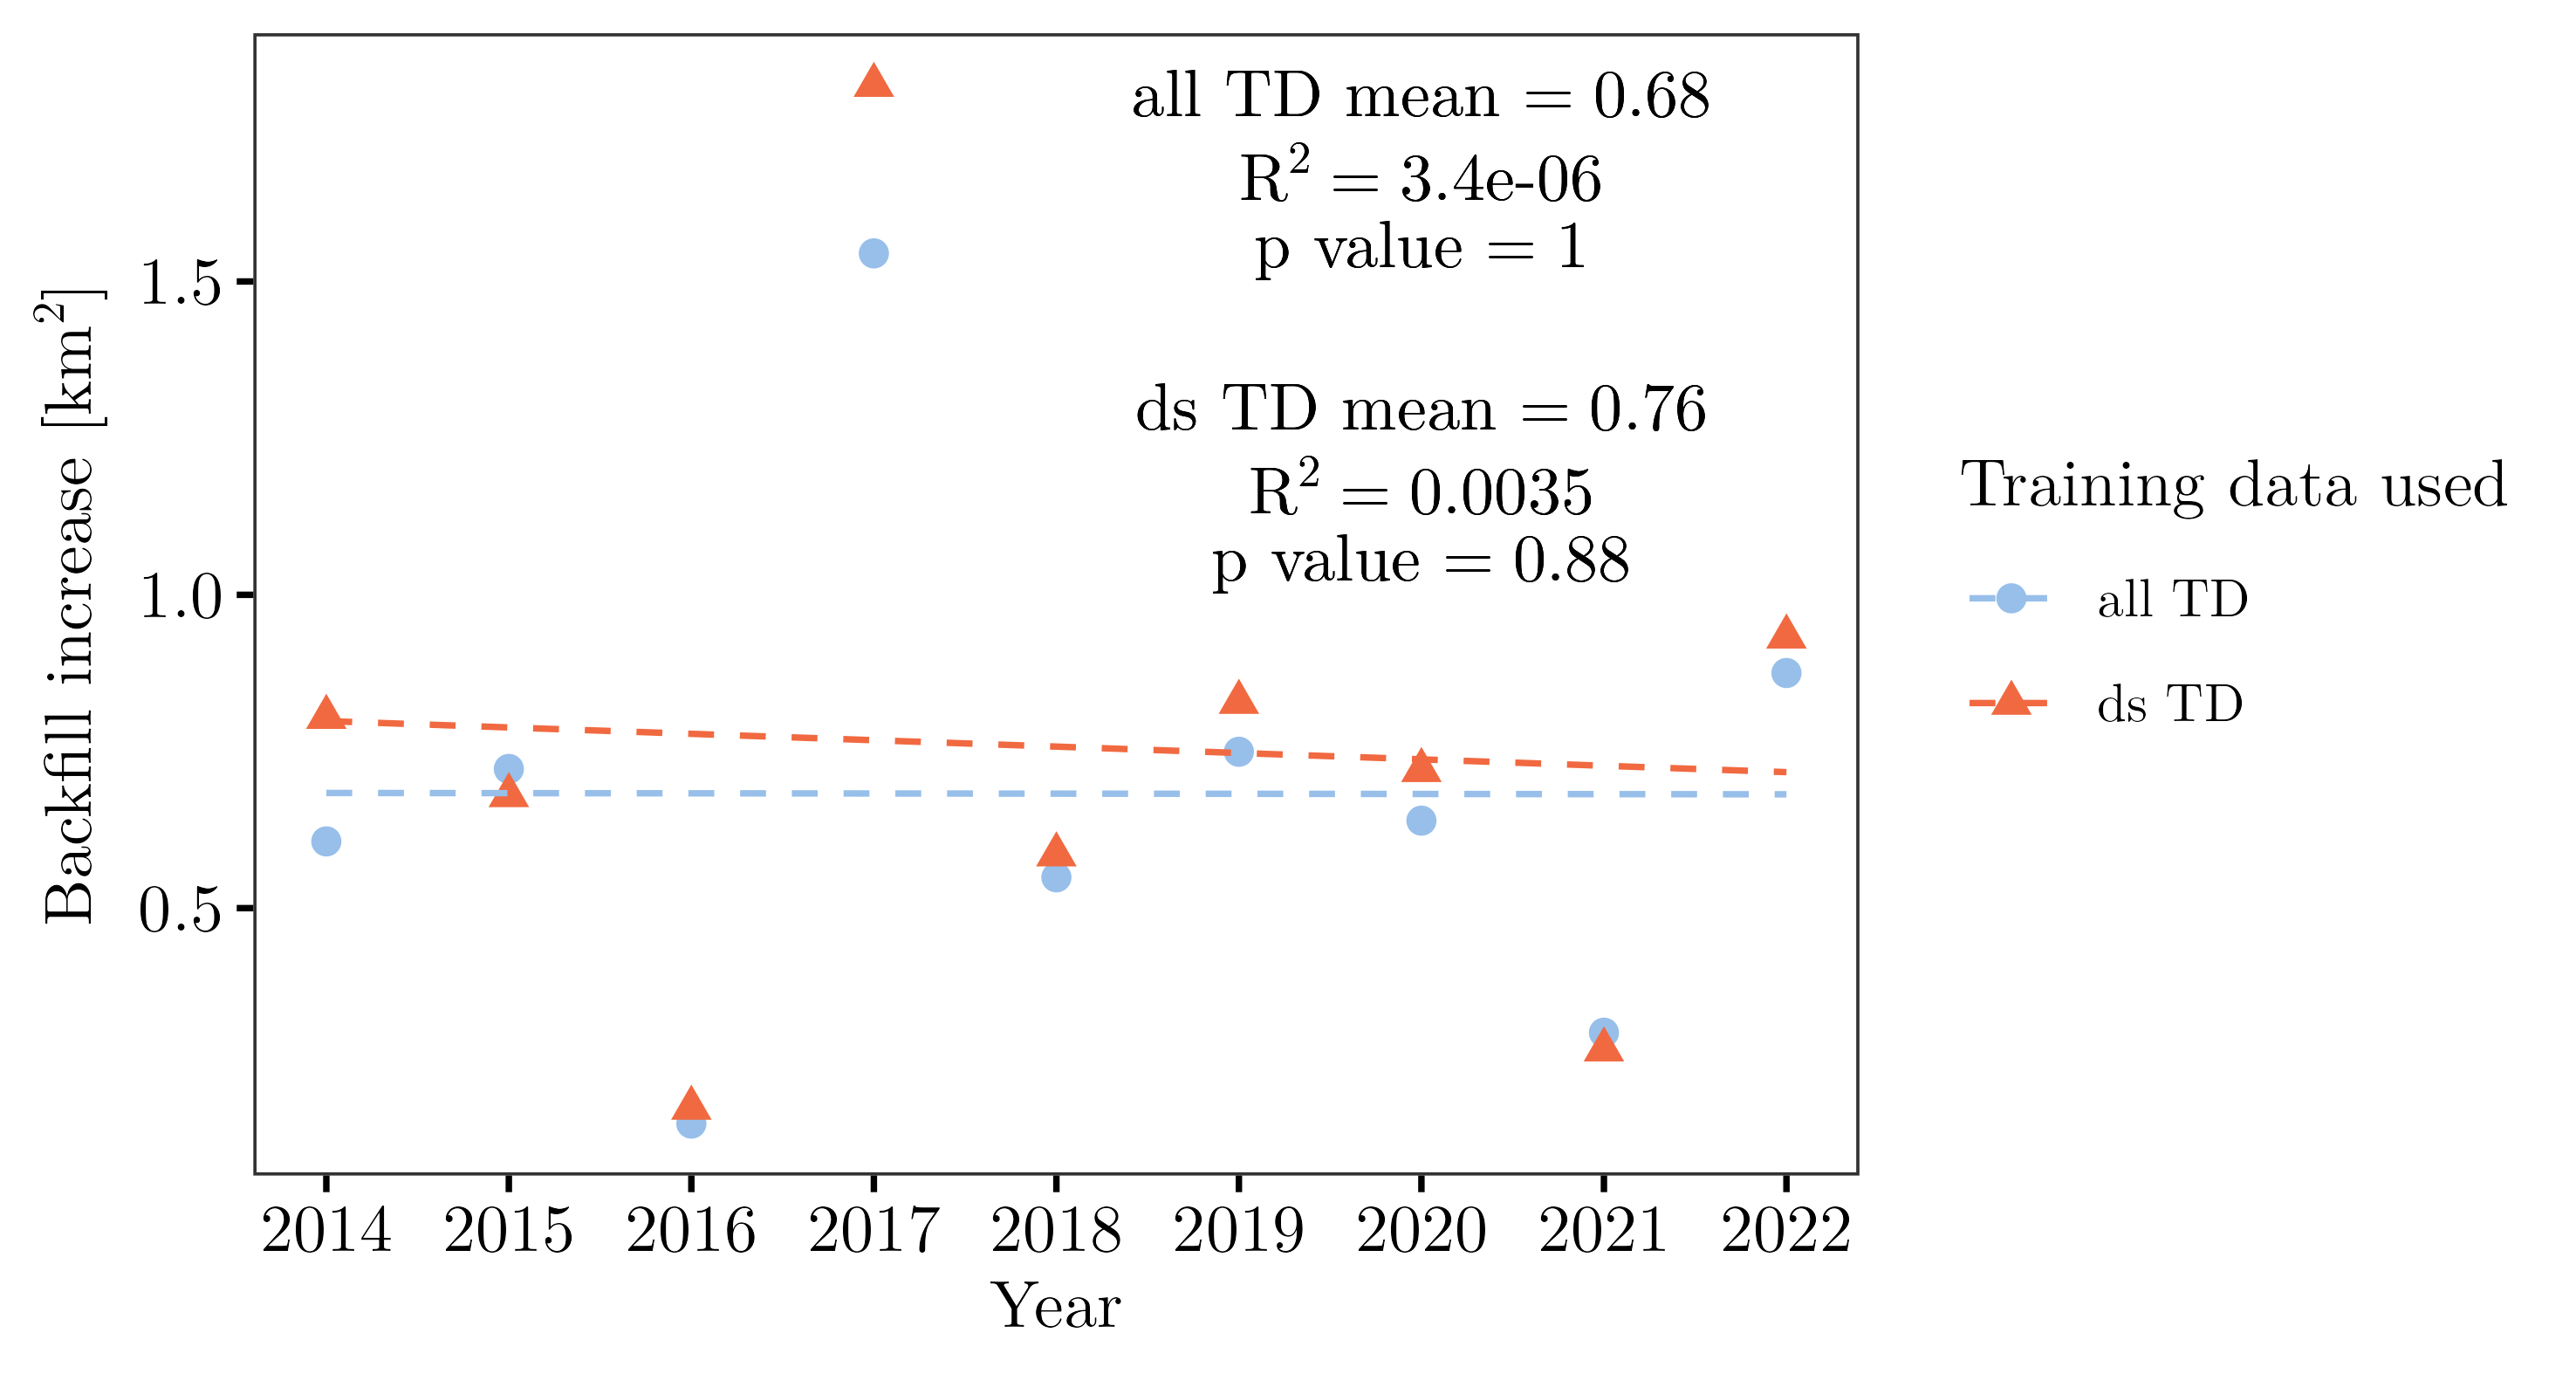
\includegraphics[width = 15cm]{figures/3_results/Backfill area increase km 2.png}
\caption{Yearly backfill area increase [km$^2$yr$^{-1}$] in the study area around Antananarivo. The years are indicative of the rainy season over which the image composites were acquired. The area values represent the increase in backfill area since the rainy season in the year before. Red triangles show the results, when using only the downsampled (ds) training data (TD), and blue dots when using all TD.}
\label{fig:areakm2}
\end{figure}

\begin{figure}[H]
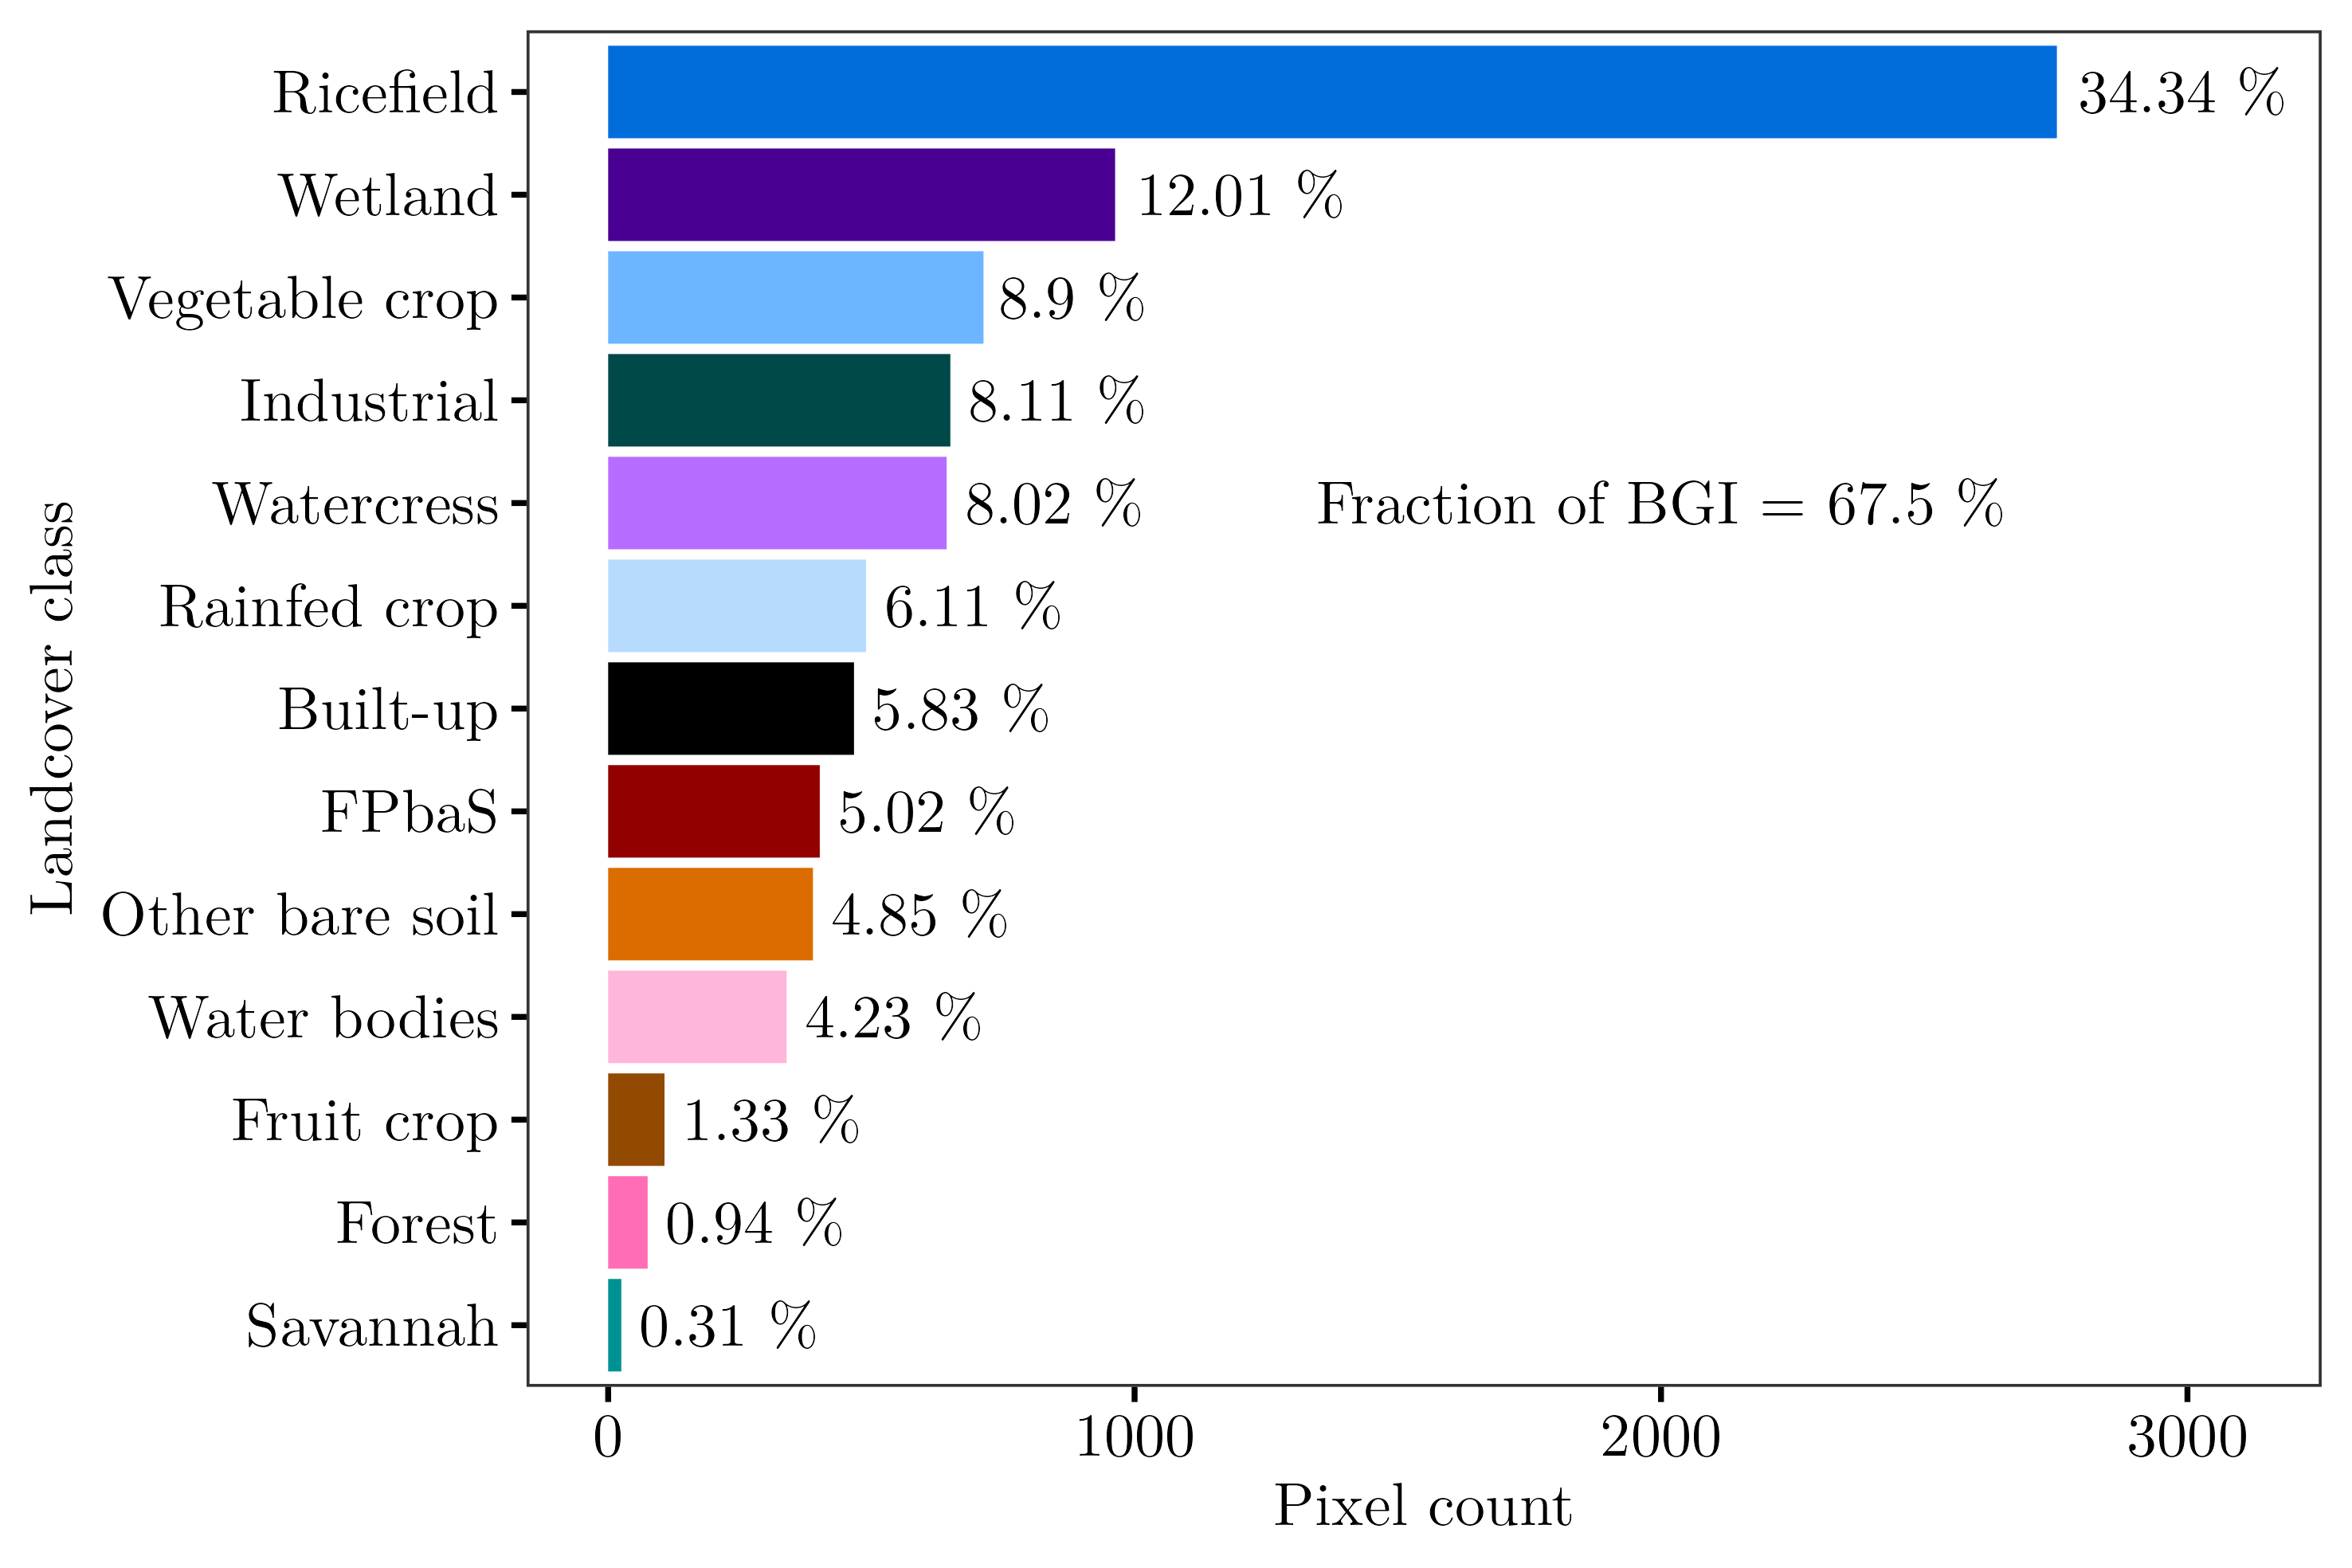
\includegraphics[width = 15cm]{figures/3_results/what was backfilled.png}
\caption{Previous year classification of backfill increase pixels over all years. The fraction of Blue and Green Infrastructure (BGI) shows the sum of ricefield, water bodies, watercress, wetland, and vegetable crop classes combined.}
\label{fig:conversionRate}
\end{figure}

\begin{rotatepage}
\begin{landscape}
\begin{figure}[H]
\includegraphics[width = 25cm]{figures/3_results/Backfill_increase_focus.png}
\caption{Distribution of identified backfill areas in all years in the study area (left). The smaller maps (indicated  in overview map) show the backfill increase per year for three specific areas. The data showing urban areas in the map is sourced from \citet{Dupuy.2019}.}
\label{fig:backfill focus area map}
\end{figure}
\end{landscape}
\end{rotatepage}

\subsection{Backfill size distribution}
Figure \ref{fig:BFtypo} indicates that most areas classified as backfill were small, spanning no more than 0.1 hectares, meaning they consist of one pixel of the classified image (30x30m). For areas starting at a larger scale (0.5 ha), the distribution is similar, but less extreme. This shows, that also smaller backfilled areas of less than one hectare in size had a considerable contribution to the yearly increase in overall backfilled area. 

\begin{figure}[H]
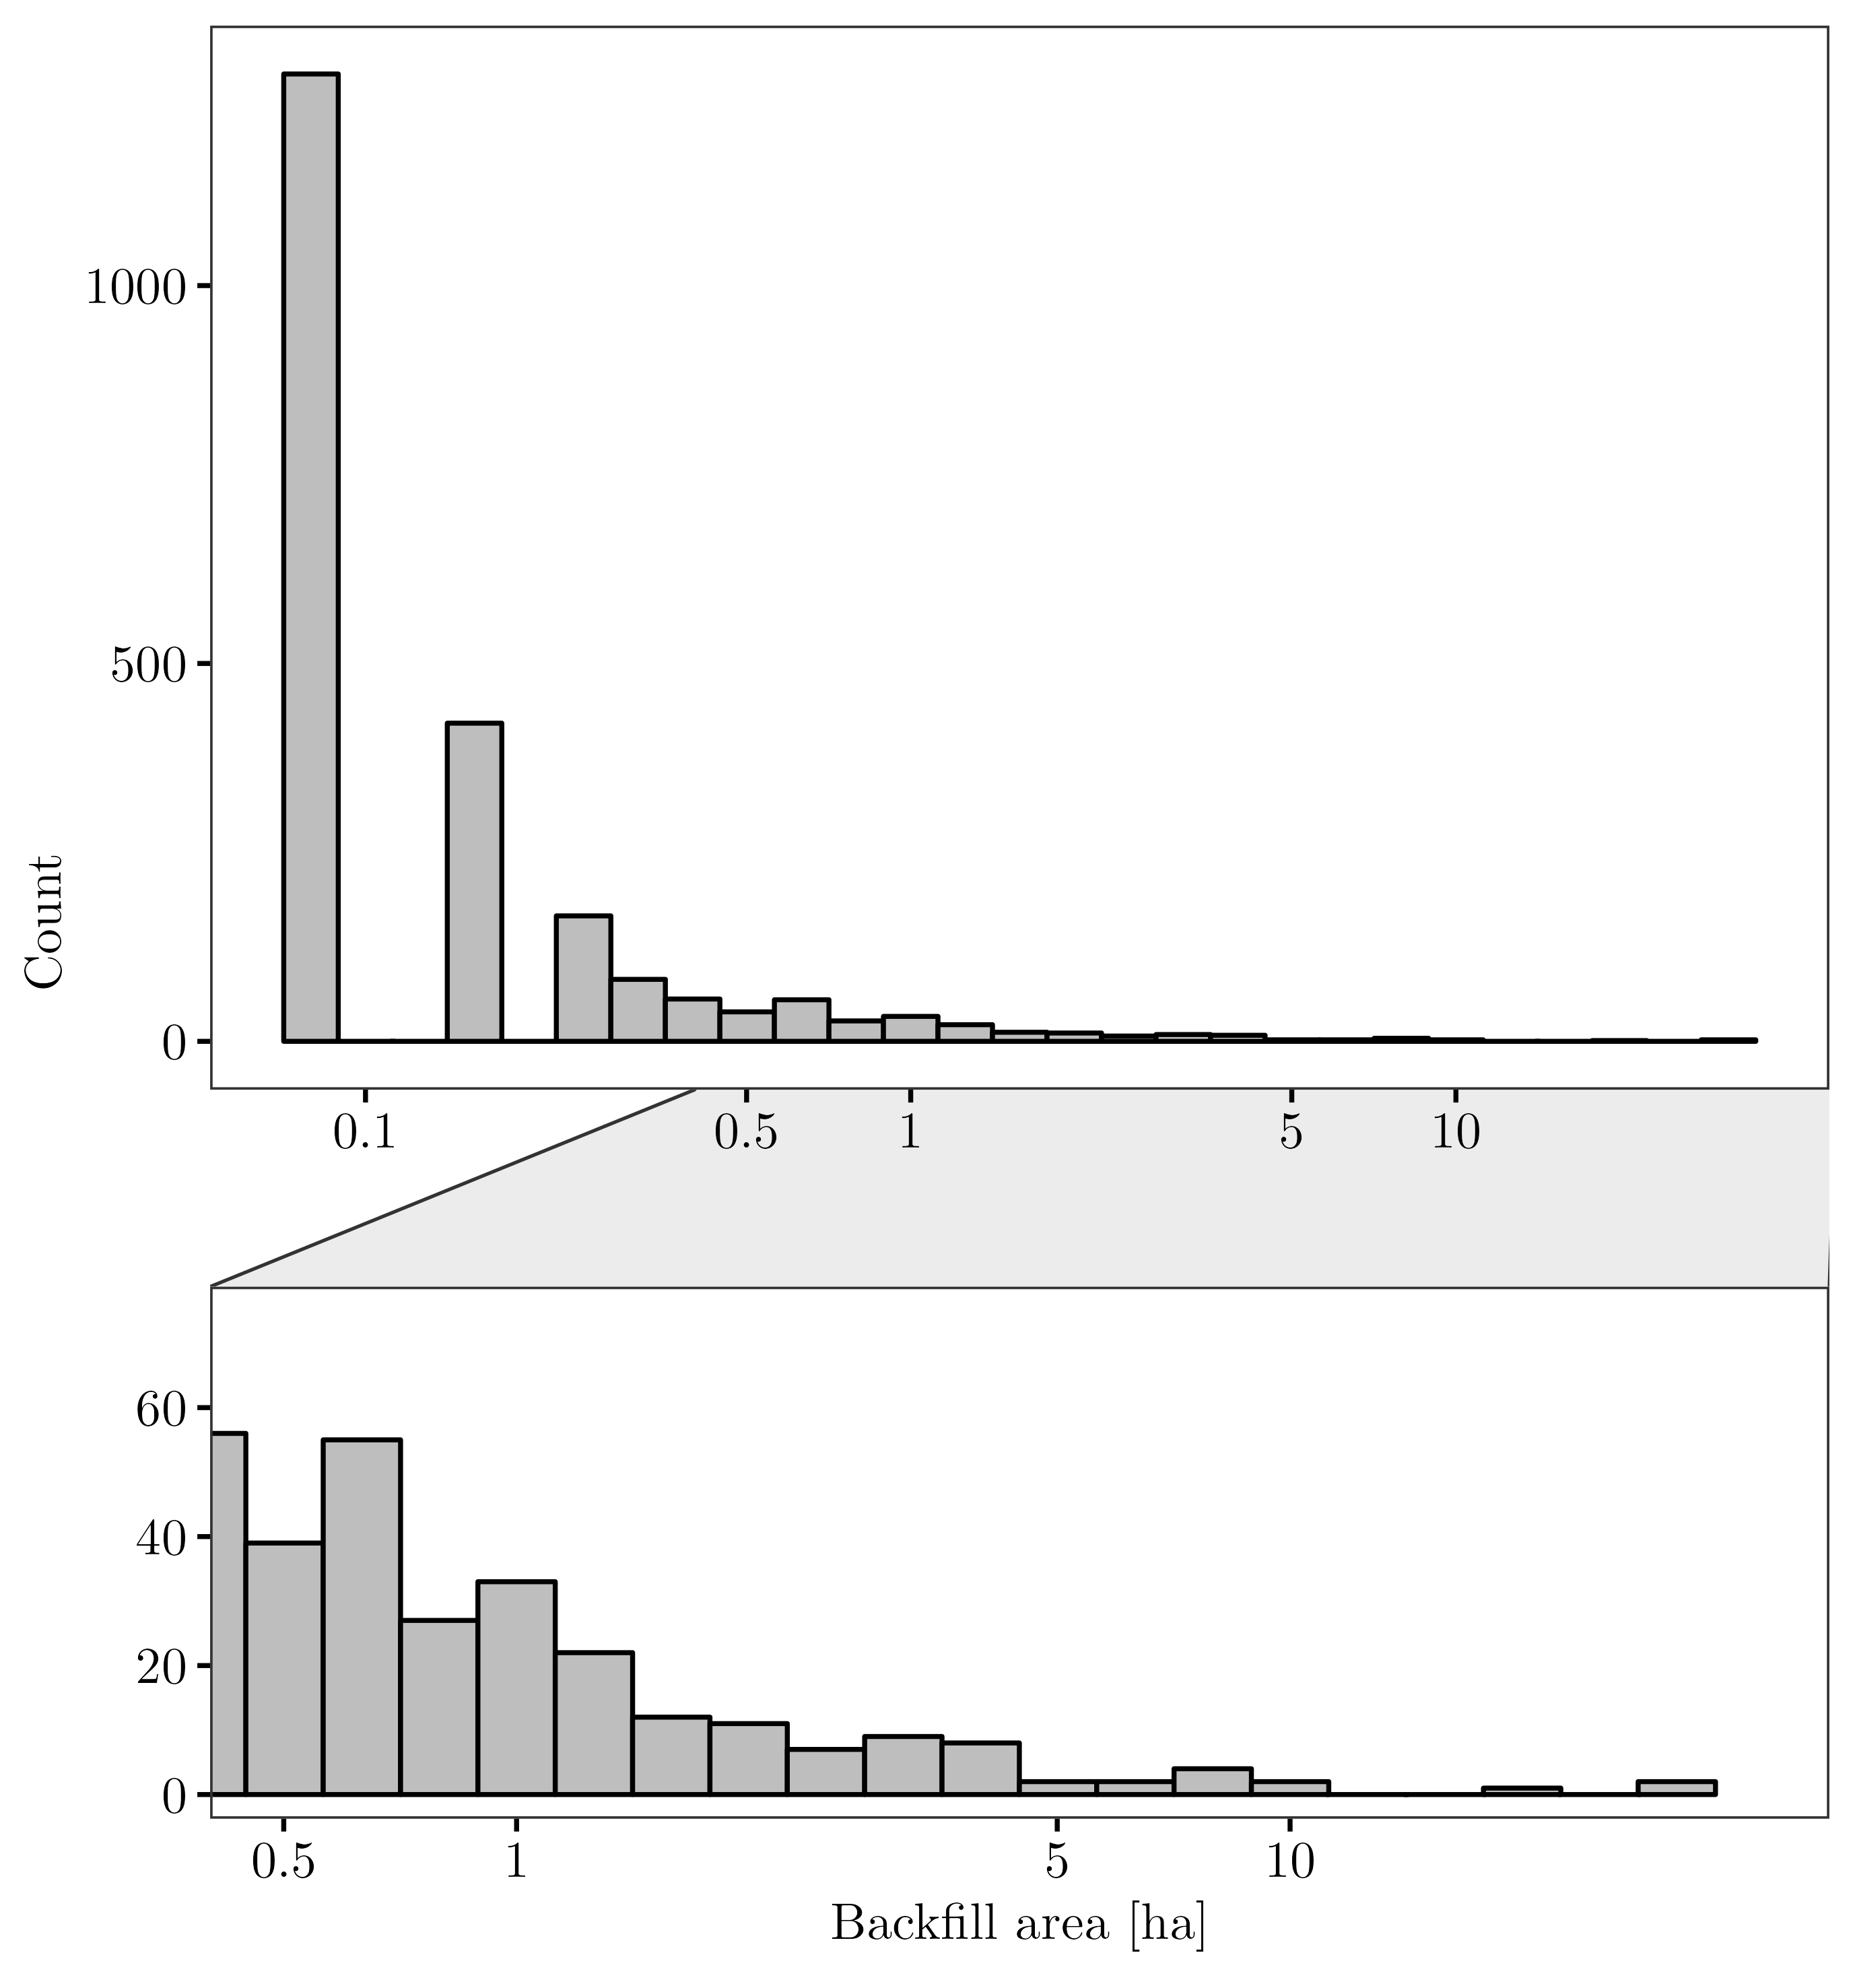
\includegraphics[width = 14cm]{figures/3_results/Backfill typology sizes_hm.png}
\caption{Size distribution among the areas classified as backfill (annual increase). A histogram of the frequency of backfills per area [ha] of the respective site. The scale is logarithmic (binwidth = x[ha]*$10^{0.1}$). The bottom part shows the right section of the plot magnified, for better recognition of the lower backfill counts.}
\label{fig:BFtypo}
\end{figure}




\section{Drivers of Backfilling} 
\subsection{All years}
Logistic regression was employed to analyze the influence of different independent variables  on backfills that occured a year later. The independent variables of this regression analysis are of two kinds. Firstly, the continuous variables of distances to other landcover classes (in the year before) and external datasets of primary and secondary roads, as well as impervious areas. And secondly,  categorical variables indicating the landcover classification in the previous year for specific chosen classes in binary (table \ref{tab:logreg_allyrs}). The model compares yearly backfill increase to a control dataset, which was randomly chosen from pixels of other landcover classes to fit the size of the backfill dataset. The industrial and built-up classes were excluded from the control dataset, assuming that once an area is urbanized or built-up, it won't be prone to being backfilled anymore.

Figure \ref{fig:logibox_allyr} shows boxplots comparing the backfills (yearly increase) to the control dataset. We can derive that backfills seem to be associated with a closer proximity to existing backfills from previous years than other landcover classes. For distances to impervious areas and roads, there is less difference between backfills  and the control data. Overall, outliers are very common for the variables. 

The results from the regression analyses, when ran over the data of all yearly increase steps, show previous year backfills as the main influencing factor (Table \ref{tab:logreg_allyrs}). However, the regression model does not fit the data very well, with an R$^2$ (Mc Fadden) of 0.11, which indicates that the model does not fully explain  the distribution and occurrence of new backfills and there could be other, unknown factors having a strong influence. Holding all other variables constant, the odds for new backfill, when multiplied by its odds ratio, decreased by 6.8 \% (OR, 0.932 | 95\% CI [0.926, 0.938]) for a unit increase (hm) in distance to already existing backfills of the year before. In all cases, previous year classification as a crop class, wetland, or water body decreased the probability of new backfills occurring a year later, whereas Built-up and industrial increased it. The independent variables were all significant, with p-values lower than 0.05.

The same regression model was run for the annual steps separately. There are high differences in model fit between the years (figure \ref{fig:logitimeseriesBF}, p. \pageref{fig:logitimeseriesBF}, A). Supporting the overall analyses, there is a significant decrease in backfill probability with increasing distance to already existing backfills for all years. This was the only variable that had a consistent OR below or above one in all years, and was also significant in all years. The other variables of distance to roads and distance to impervious surfaces have odds ratios that are generaly scattered aound the value of one between the different years. The high degree of variability between years is shown both by the value of Mc Fadden's R$^2$ and the varying odds ratios of the backfill class between different years in the plot. High values of R$^2$ seem to coincide with more meaningful odds ratios for the distance to previous backfills (Figure \ref{fig:logitimeseriesBF}, A and B), again underlining the relative importance of this class for the model.

%\begin{figure}[H]
%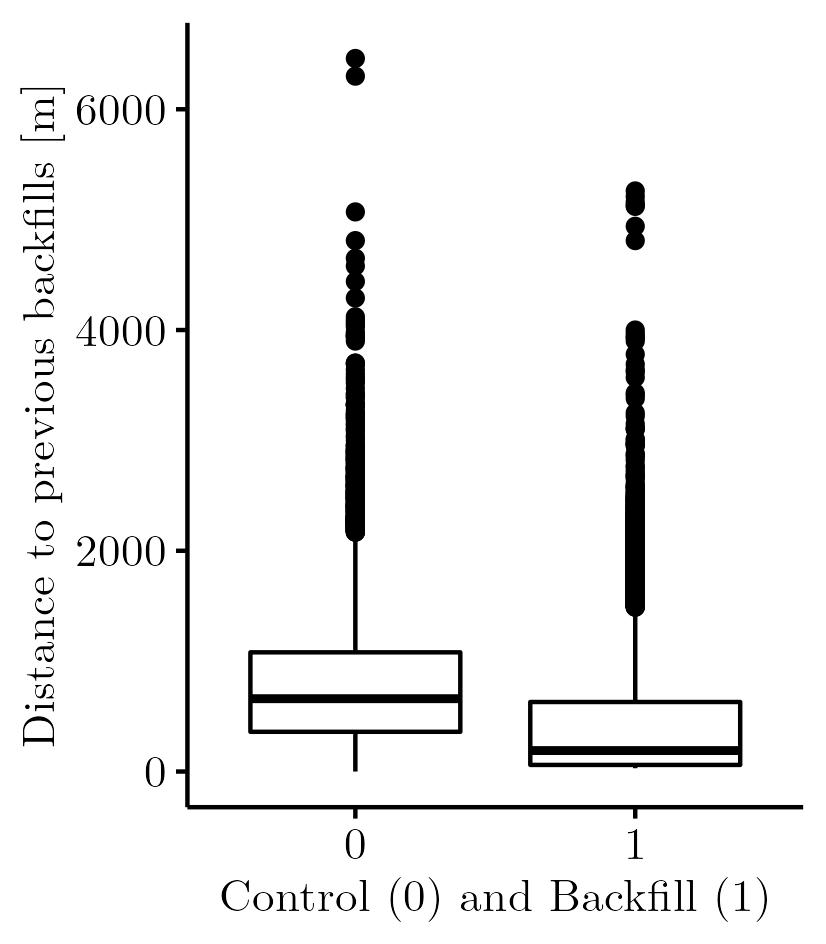
\includegraphics[width = 7 cm]{figures/boxplot backfill logi.jpg}
%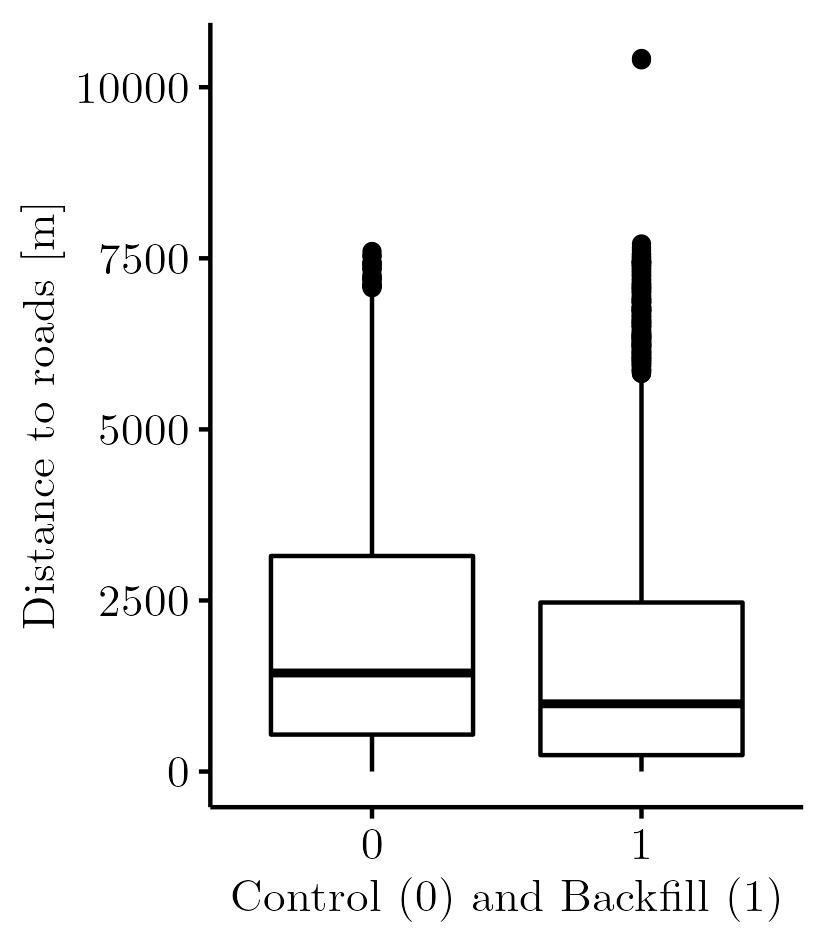
\includegraphics[width = 7 cm]{figures/boxplot roads logi.jpg}
%\caption{Comparison of the yearly backfill increments and control with respect to the distance [m] to backfills in the %previous year and roads.}
%\label{fig:logibox}
%\end{figure}

\begin{figure}[H]
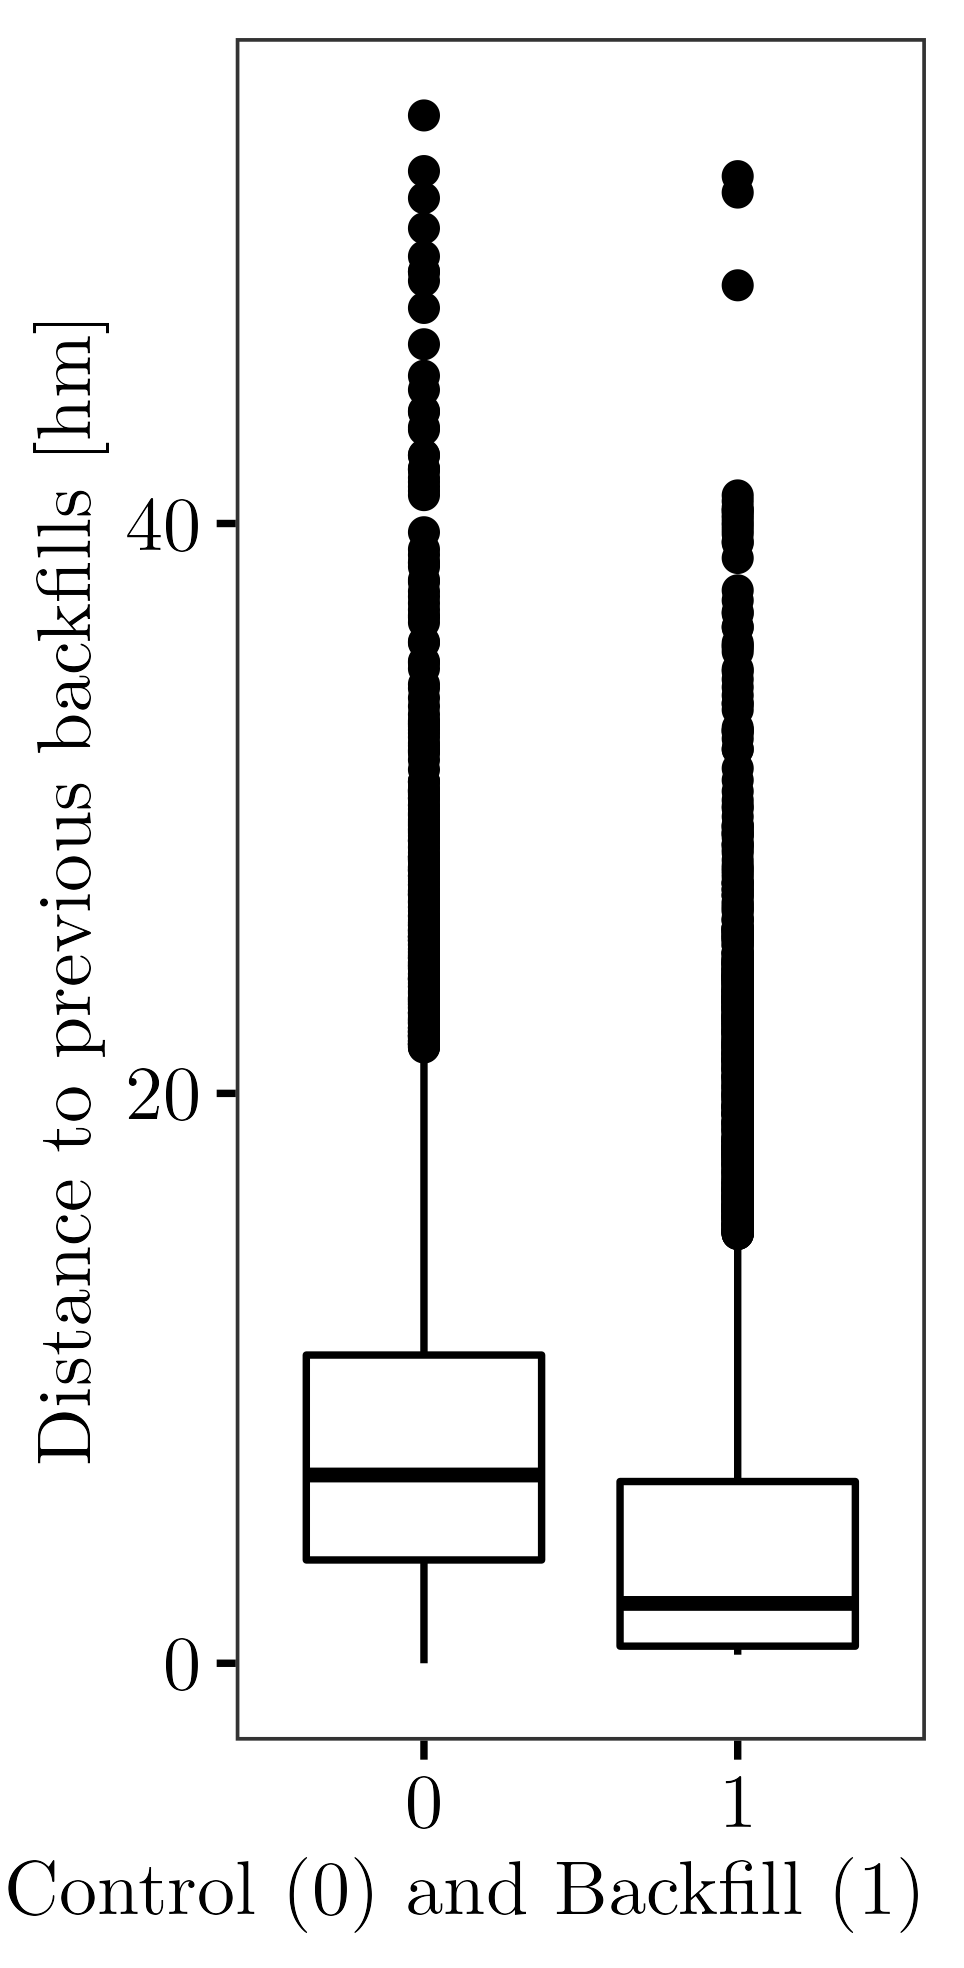
\includegraphics[width = 4.9 cm]{figures/3_results/boxplot backfill logi.png}
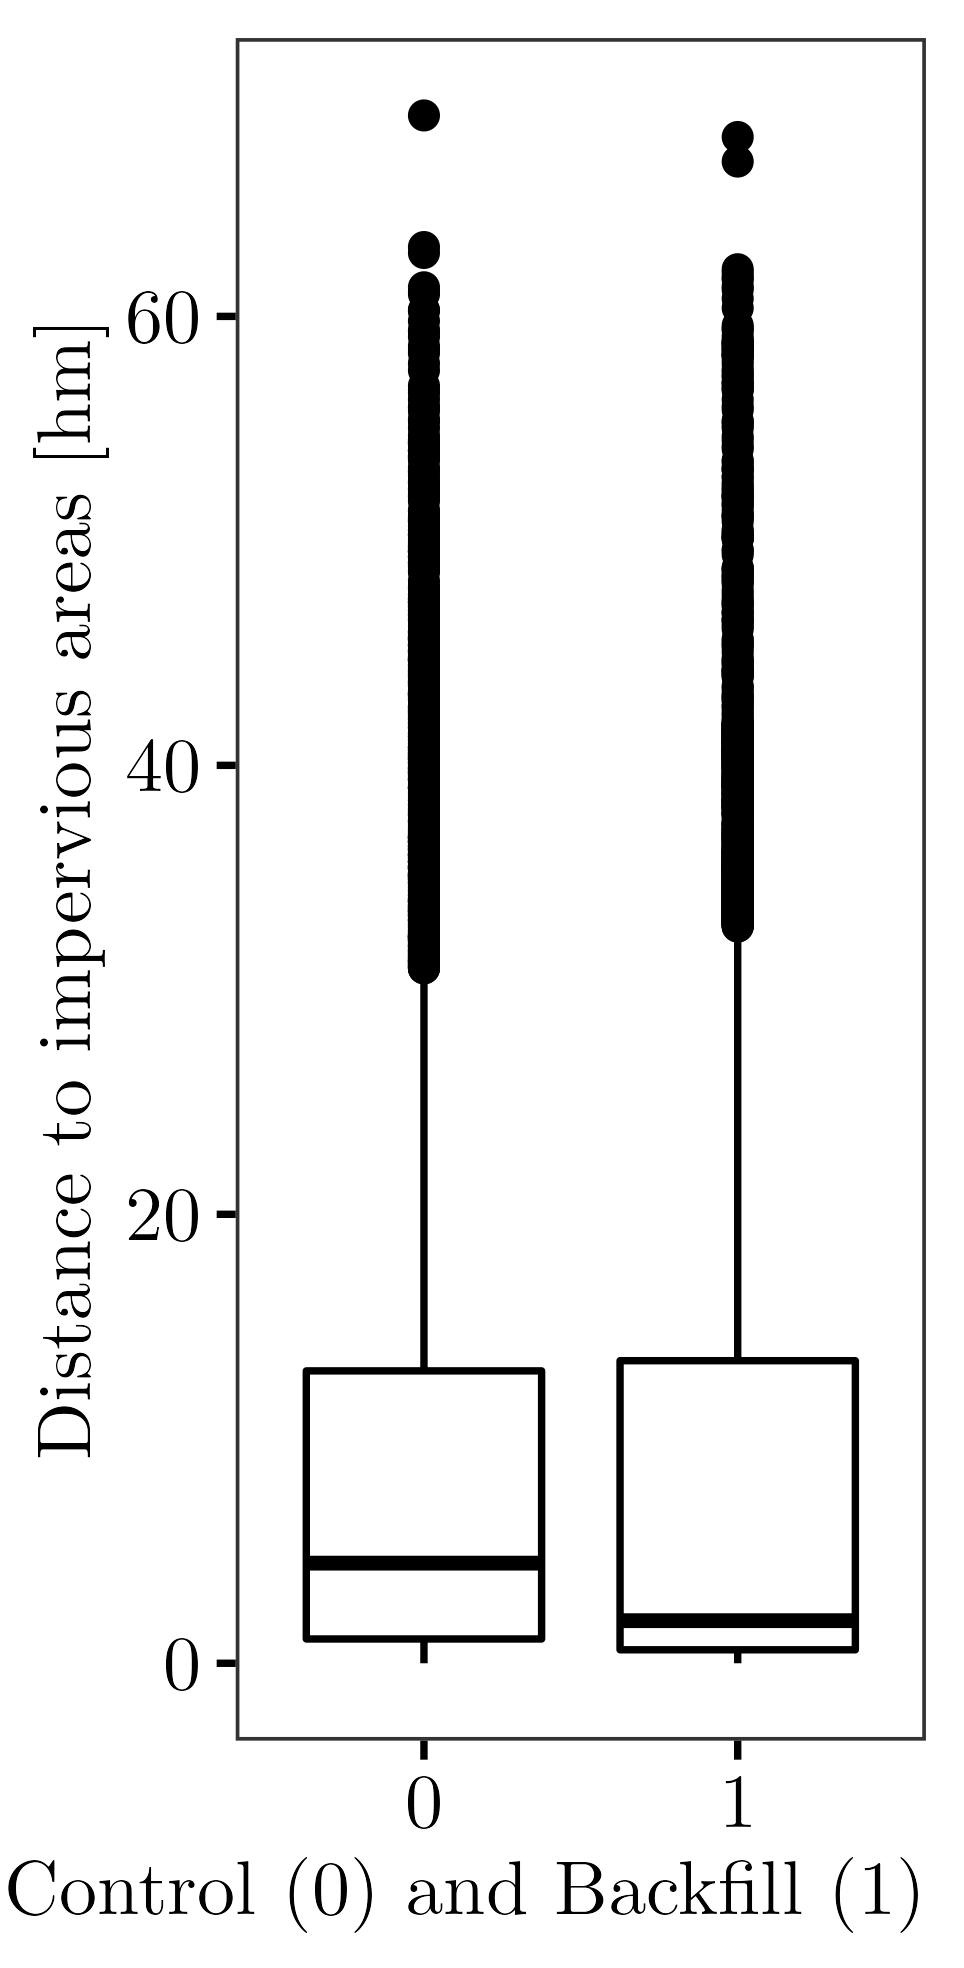
\includegraphics[width = 4.9 cm]{figures/3_results/boxplot Imperv logi.png}
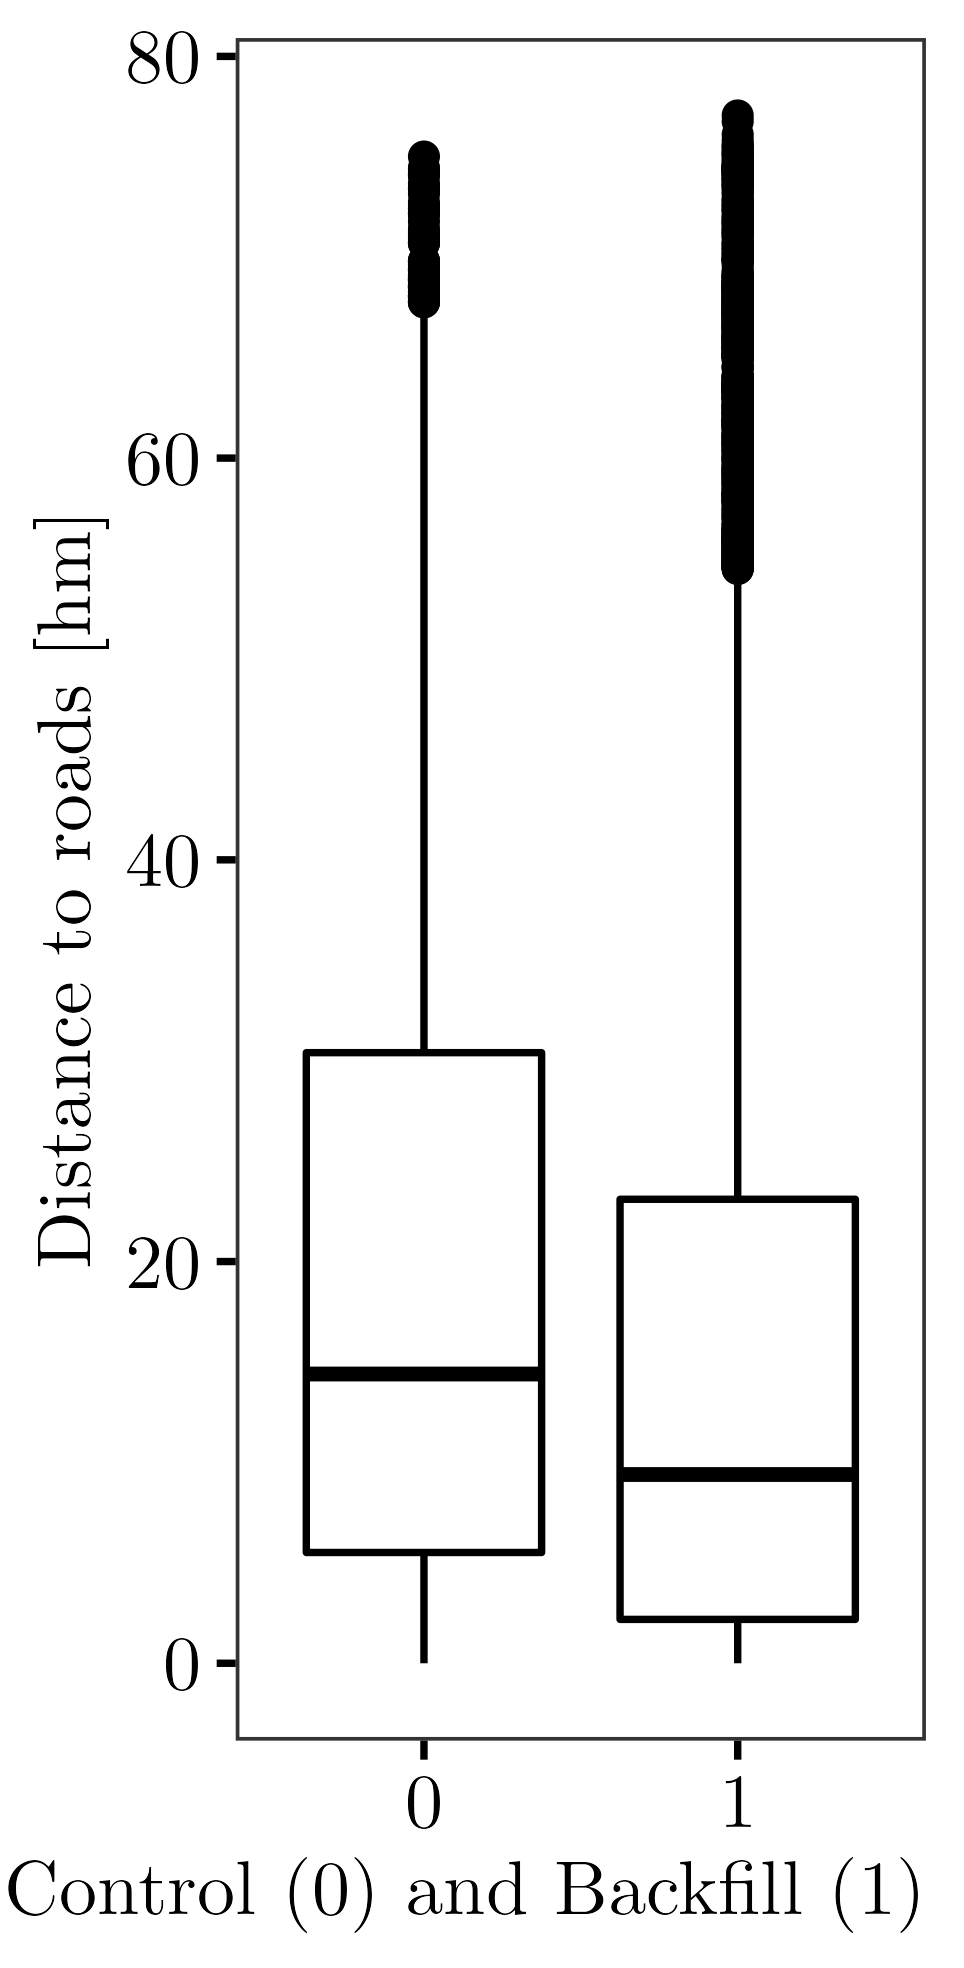
\includegraphics[width = 4.9 cm]{figures/3_results/boxplot roads logi.png}
\caption{Comparison of the yearly backfill increments and control with respect to the distance [m] to backfills in the previous year and roads for the year 2018 and distances to other landcovers.}
\label{fig:logibox_allyr}
\end{figure}

\begin{table}[H]
\caption{Summary of the logistic regression using data from all timesteps. For all independent variables used, the odds ratio (OR), lower and upper boundaries (Low, Up) of the 95\% confidence interval, variable importance (VI) and the p - value (P) are given. The overall analysis has a pseudo R$^2$ (Mc Fadden) of 0.11.}
\centering
\begin{tabular}{c c c c c c c}
  \hline
 Unit & Variables & OR & Low & Up & VI & P \\ 
  \hline
%m.a.s.l. [m] &  Elevation & 1.016 & 1.0053 & 1.0268 & 2.9323 & 0.00336 \\ 
%Slope [°] & Slope & 1.0057 & 0.984 & 1.028 & 0.5121 & 0.609 \\ 
%\hline
 \multirow{10}{3cm}{Distance [hm] to land cover in the previous year} 
& Backfill & 0.932 & 0.926 & 0.938 & 21 & *** \\ 
  & Built-up & 1.066 & 1.049 & 1.084 & 7.6 & *** \\ 
  & Impervious areas & 1.025 & 1.02 & 1.03 & 9.4 & *** \\ 
  & Industrial & 0.988 & 0.978 & 0.999 & 2.2 & * \\ 
  & Ricefield & 1.106 & 1.016 & 1.204 & 2.3 & * \\ 
  & Roads & 0.986 & 0.982 & 0.989 & 8.1 & *** \\ 
  & Vegetable crop & 0.805 & 0.782 & 0.829 & 14.4 & *** \\ 
  & Water bodies & 0.949 & 0.94 & 0.959 & 10 & *** \\ 
  & Watercress & 0.913 & 0.896 & 0.93 & 9.4 & *** \\ 
  & Wetland & 0.93 & 0.899 & 0.962 & 4.2 & *** \\
                    \hline
\multirow{6}{3cm}{Previous year classification (factor of 0/1)} 
  & Built-up & 1.431 & 1.192 & 1.717 & 3.9 & *** \\ 
  & Industrial & 5.797 & 4.507 & 7.456 & 13.7 & *** \\ 
  & Ricefield & 0.744 & 0.664 & 0.834 & 5.1 & *** \\ 
  & Vegetable crop & 0.653 & 0.567 & 0.752 & 5.9 & *** \\ 
  & Water bodies & 0.455 & 0.381 & 0.544 & 8.7 & *** \\ 
  & Watercress & 0.5 & 0.435 & 0.575 & 9.7 & *** \\ 
  & Wetland & 0.575 & 0.504 & 0.656 & 8.2 & *** \\ 
   \hline
   \multicolumn{7}{c}{p values: \qquad *** < 0.001;\quad ** < 0.01;\quad * < 0.05;\quad . < 0.1 }\\
   \hline
\end{tabular}

\label{tab:logreg_allyrs}
\end{table}




    %\draw (0, 0) node[inner sep=0] {\includegraphics[width=4cm]{imagefile.png}};
    %\draw (1, 1) node {Hello world};


\begin{figure}[H]
\begin{tikzpicture}
%\node(GEE)at (6cm,-12.75cm)[color=red!80]{R/ R-Studio};
\draw(0, 0.125cm) node[inner sep=0]{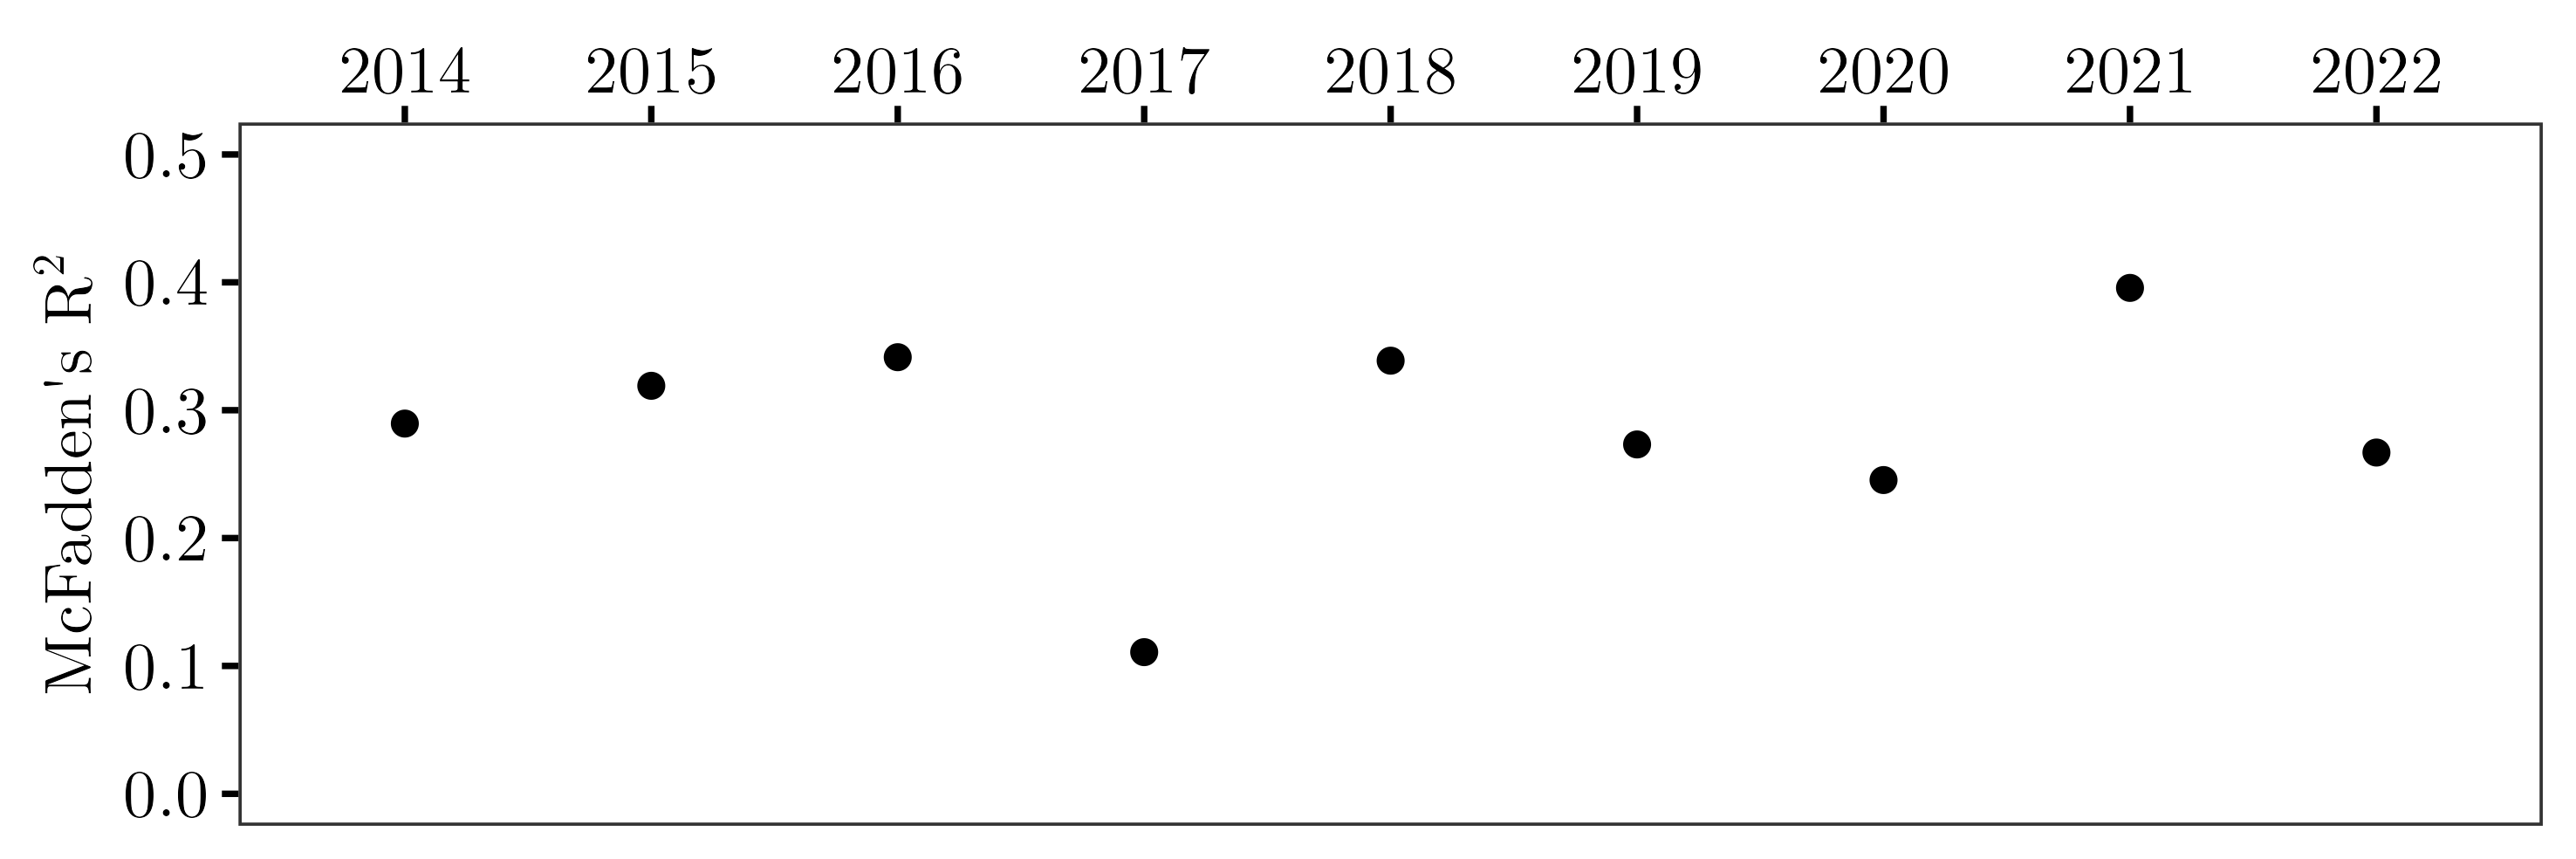
\includegraphics[width = 15 cm]{figures/3_results/logreg_year_Rsq.png}};\\
\node(A)at (-5.75cm,1.625cm)[]{\Large\textbf{A}};

\draw(0, -5cm) node[inner sep=0]{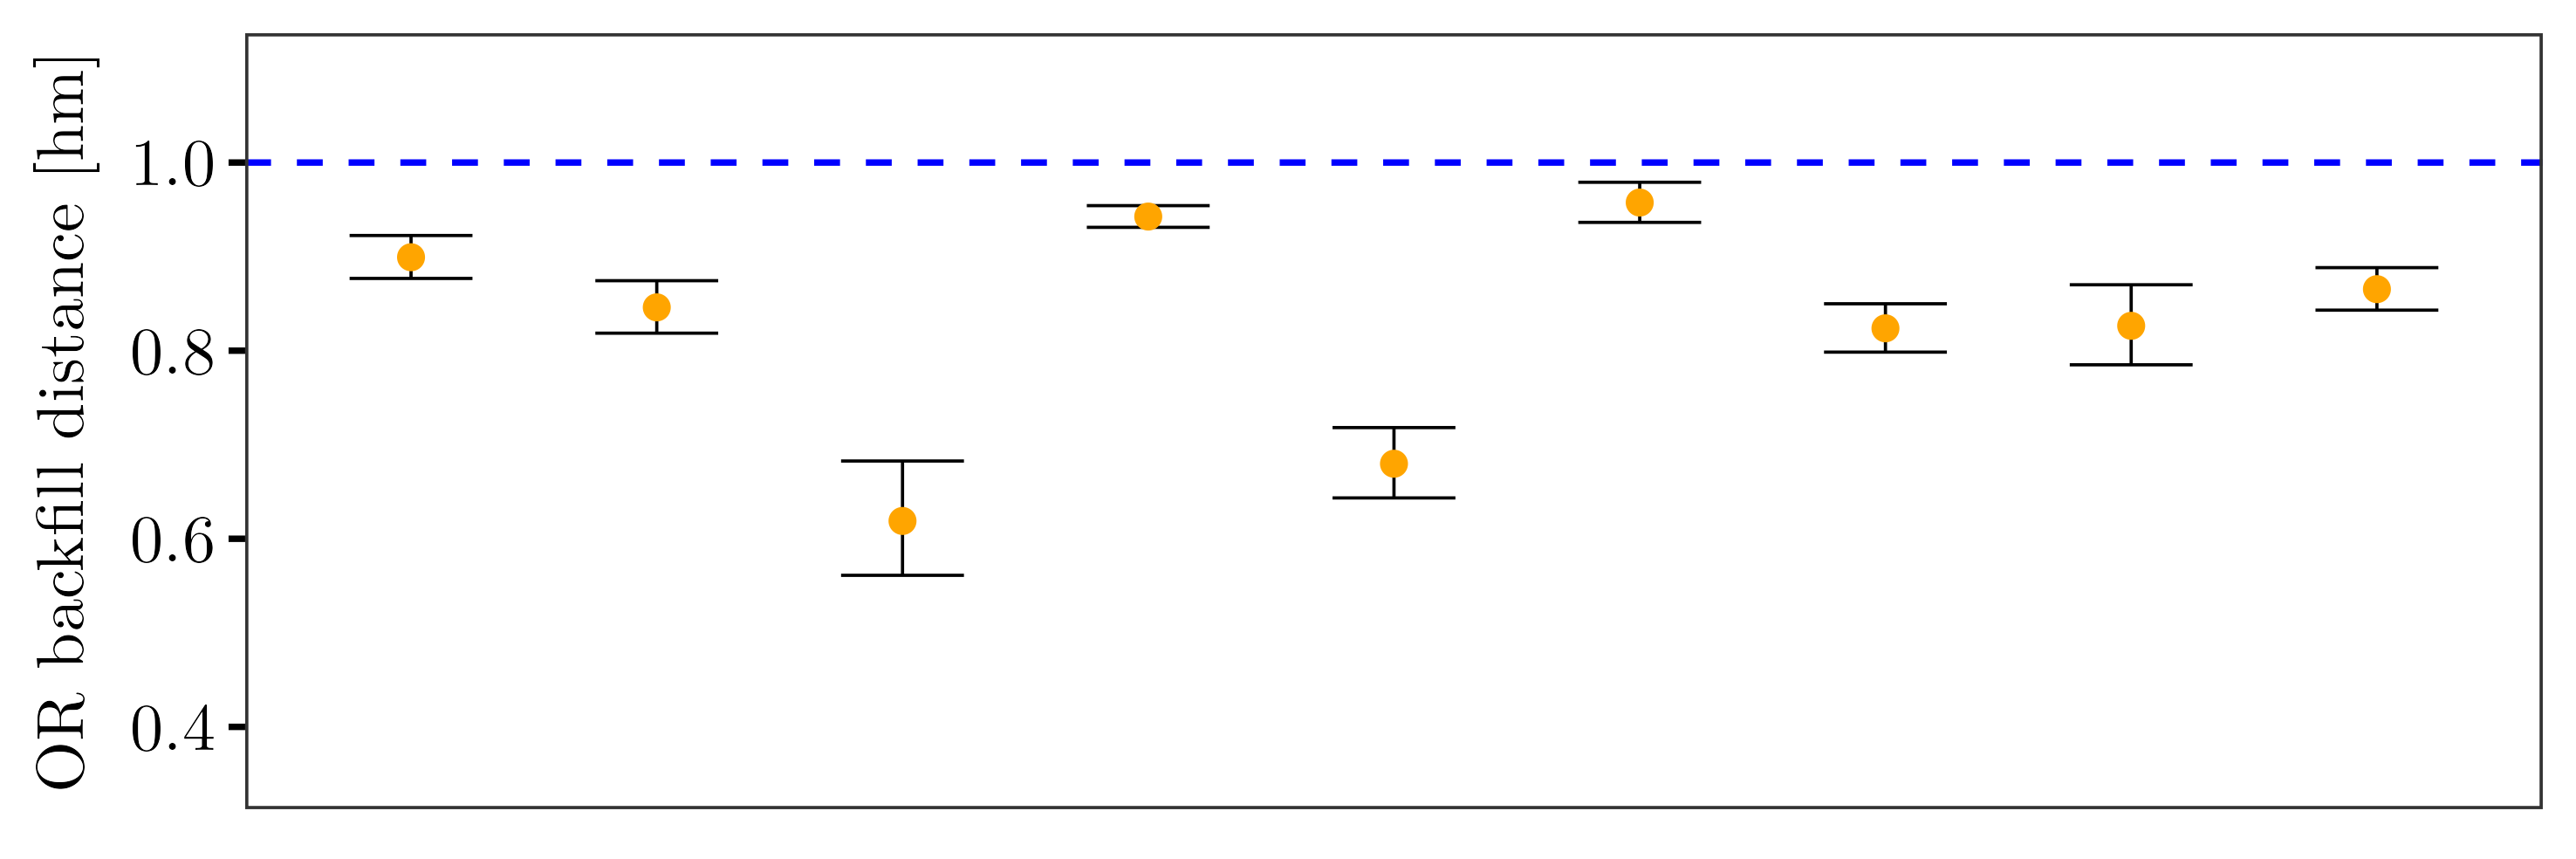
\includegraphics[width = 15 cm]{figures/3_results/logreg_year_BFdist.png}};\\
\node(B)at (-5.75cm,-3cm)[]{\Large\textbf{B}};

\draw(0, -10cm) node[inner sep=0]{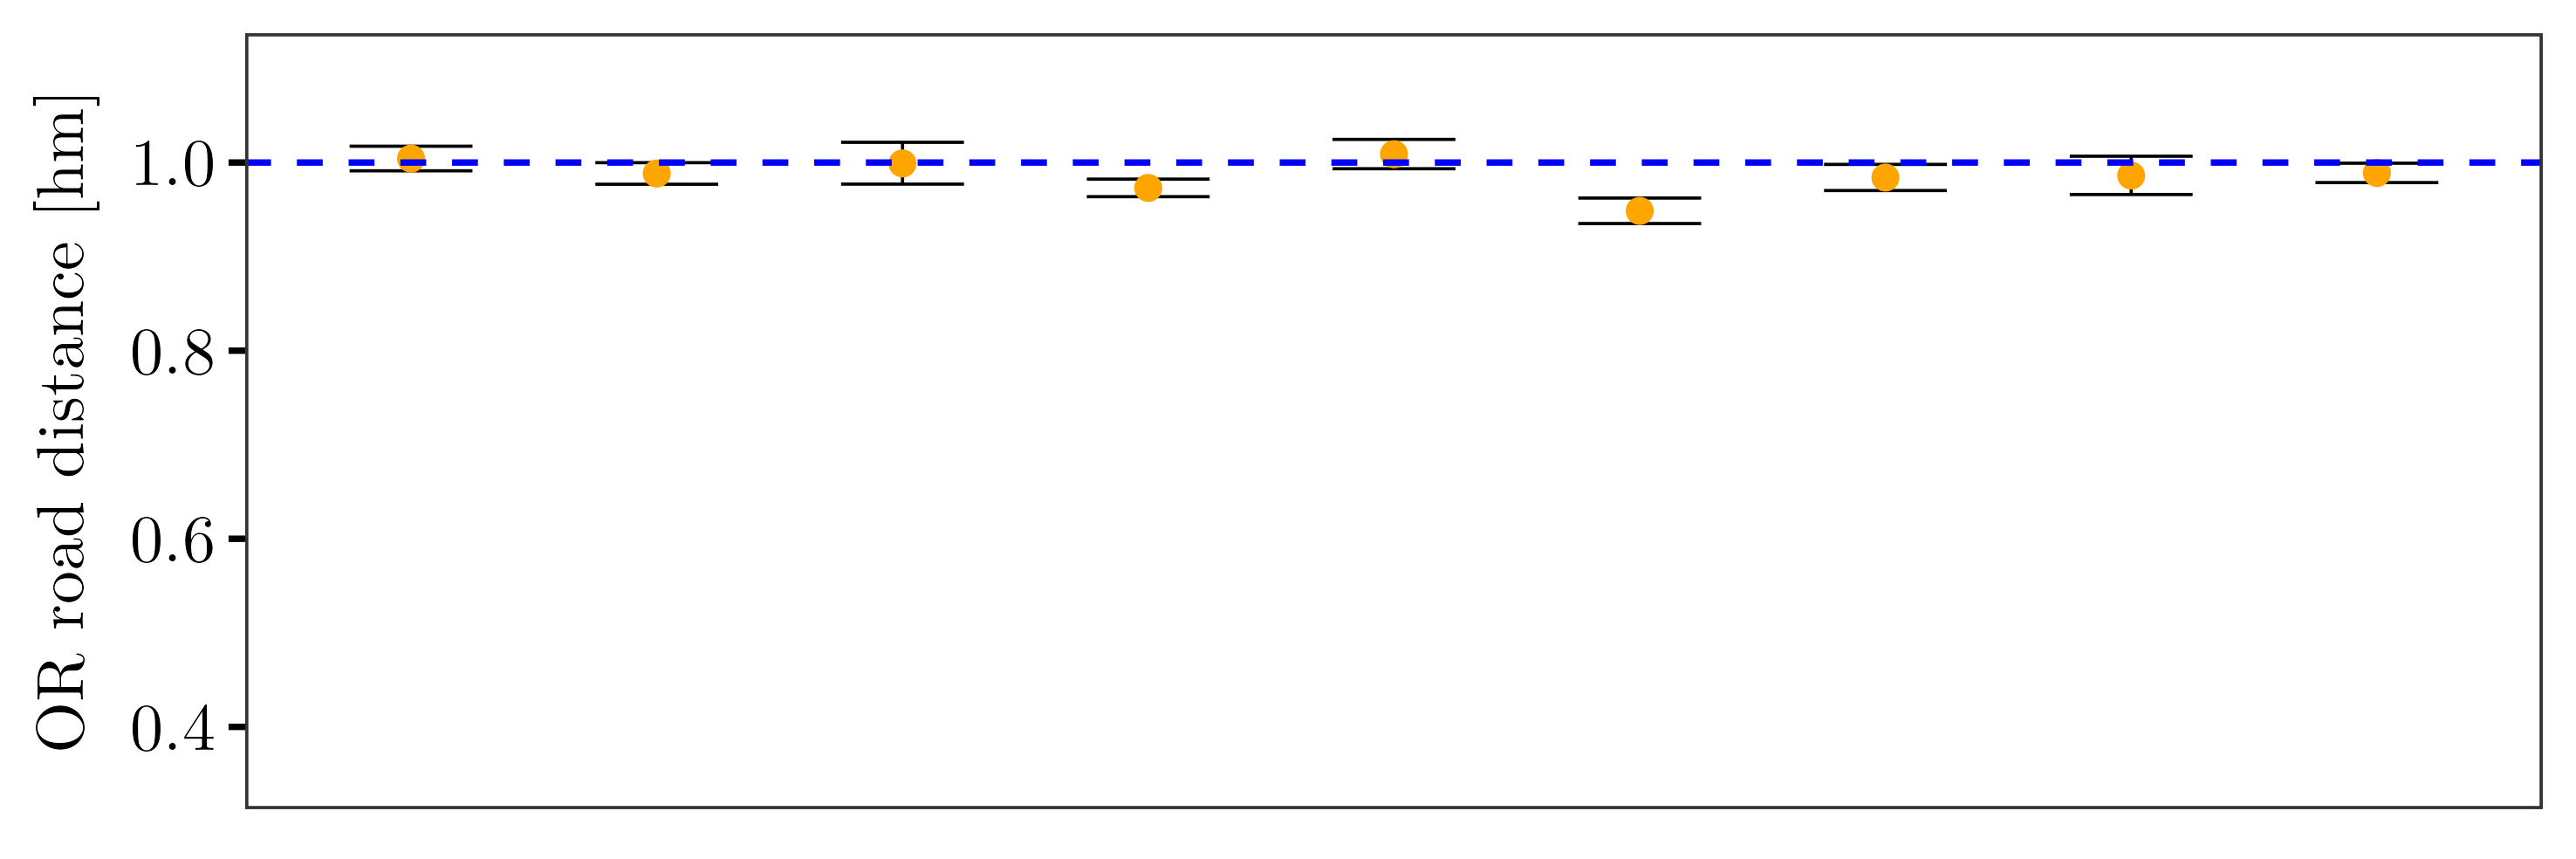
\includegraphics[width=15cm]{figures/3_results/logreg_year_Roadist.png}};\\
\node(C)at (-5.75cm,-8cm)[]{\Large\textbf{C}};

\draw(0, -15.5cm) node[inner sep=0]{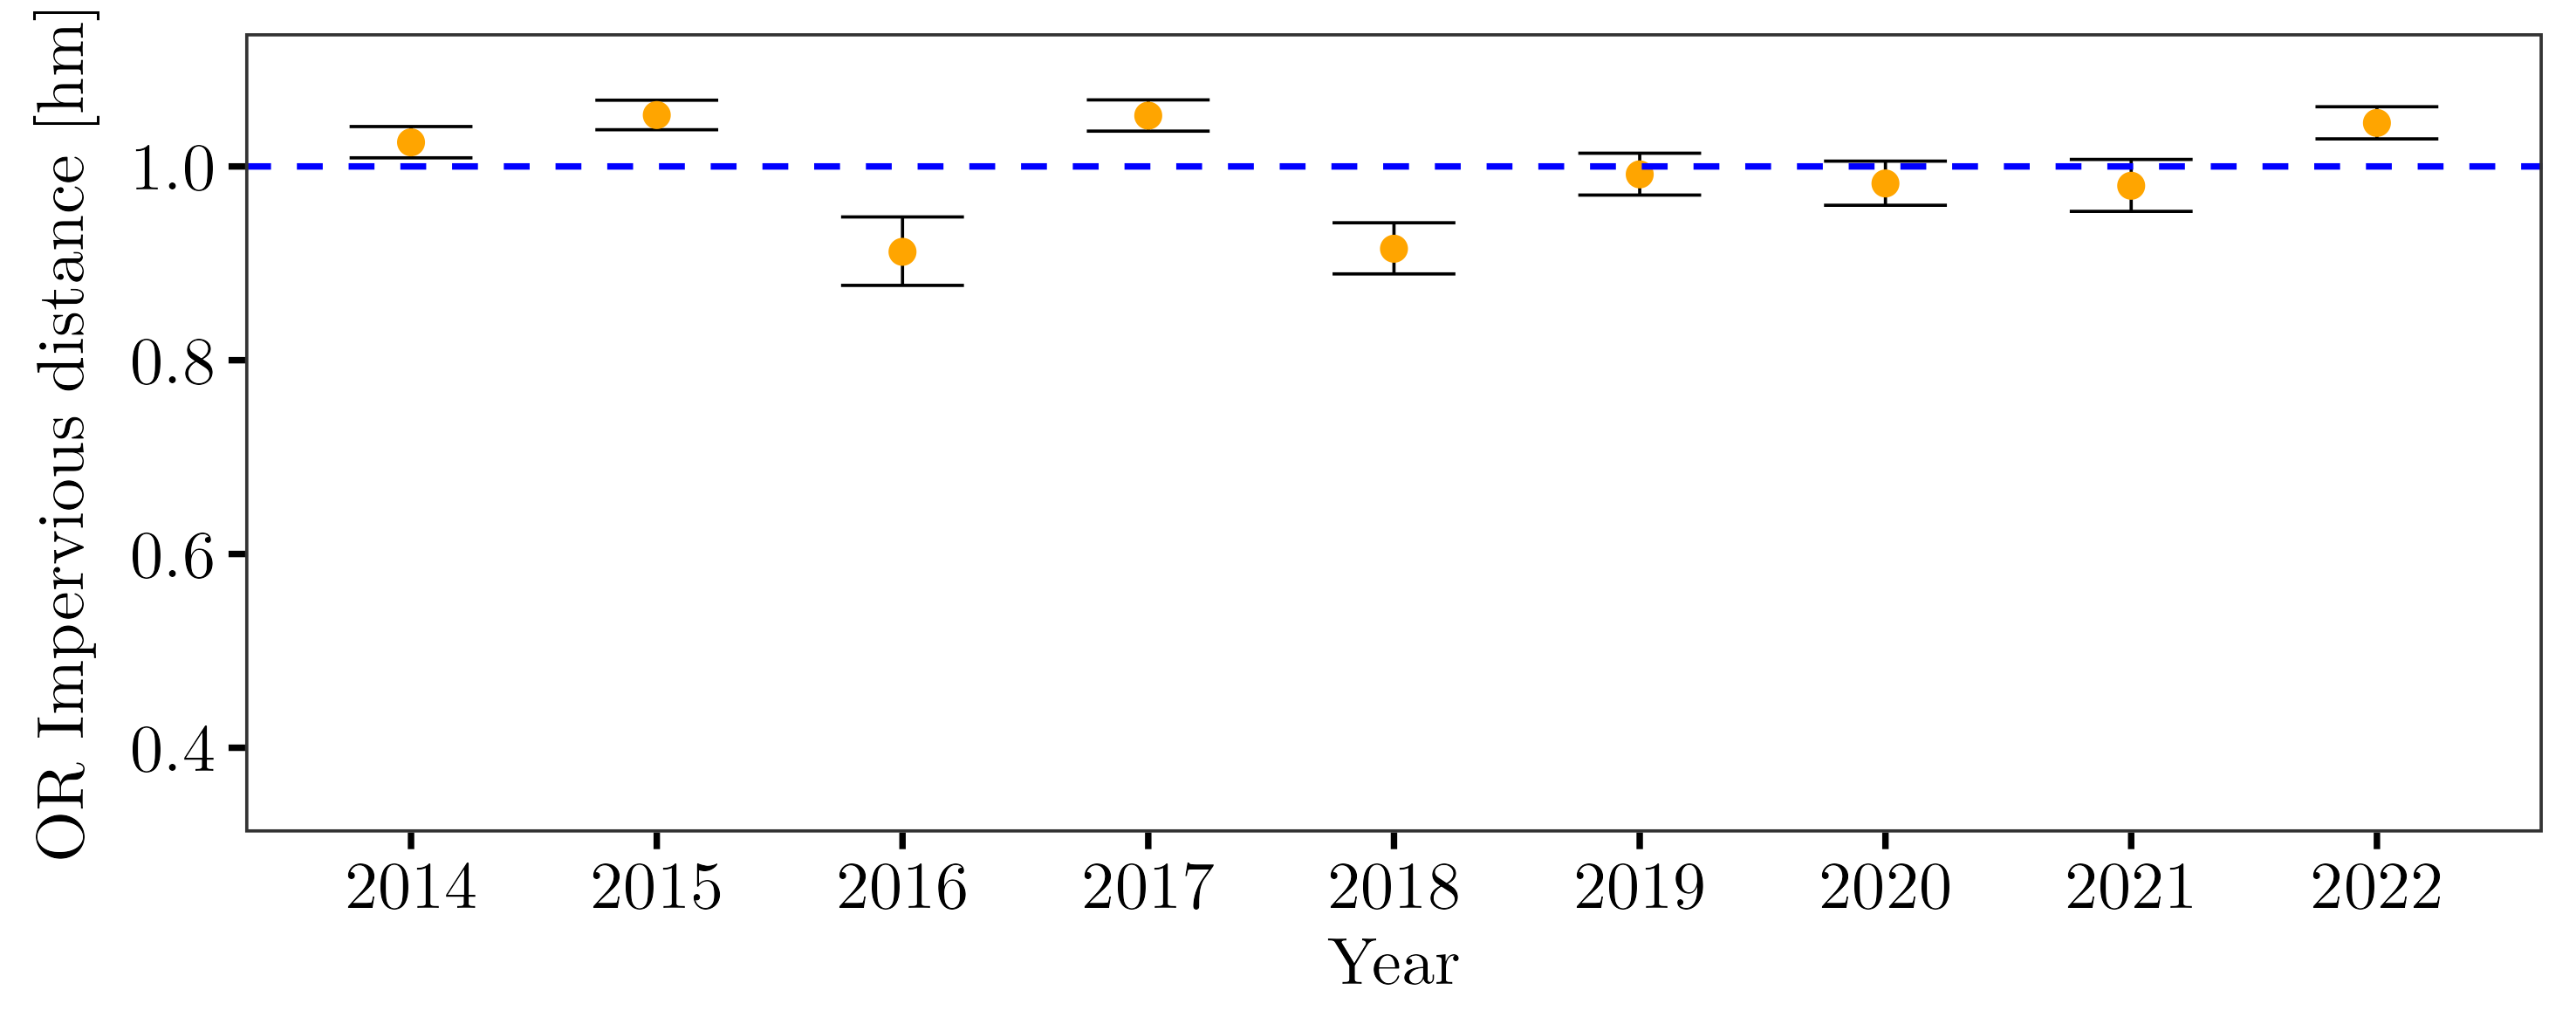
\includegraphics[width=15cm]{figures/3_results/logreg_year_Imperv.png}};\\
\node(D)at (-5.75cm,-13cm)[]{\Large\textbf{D}};
%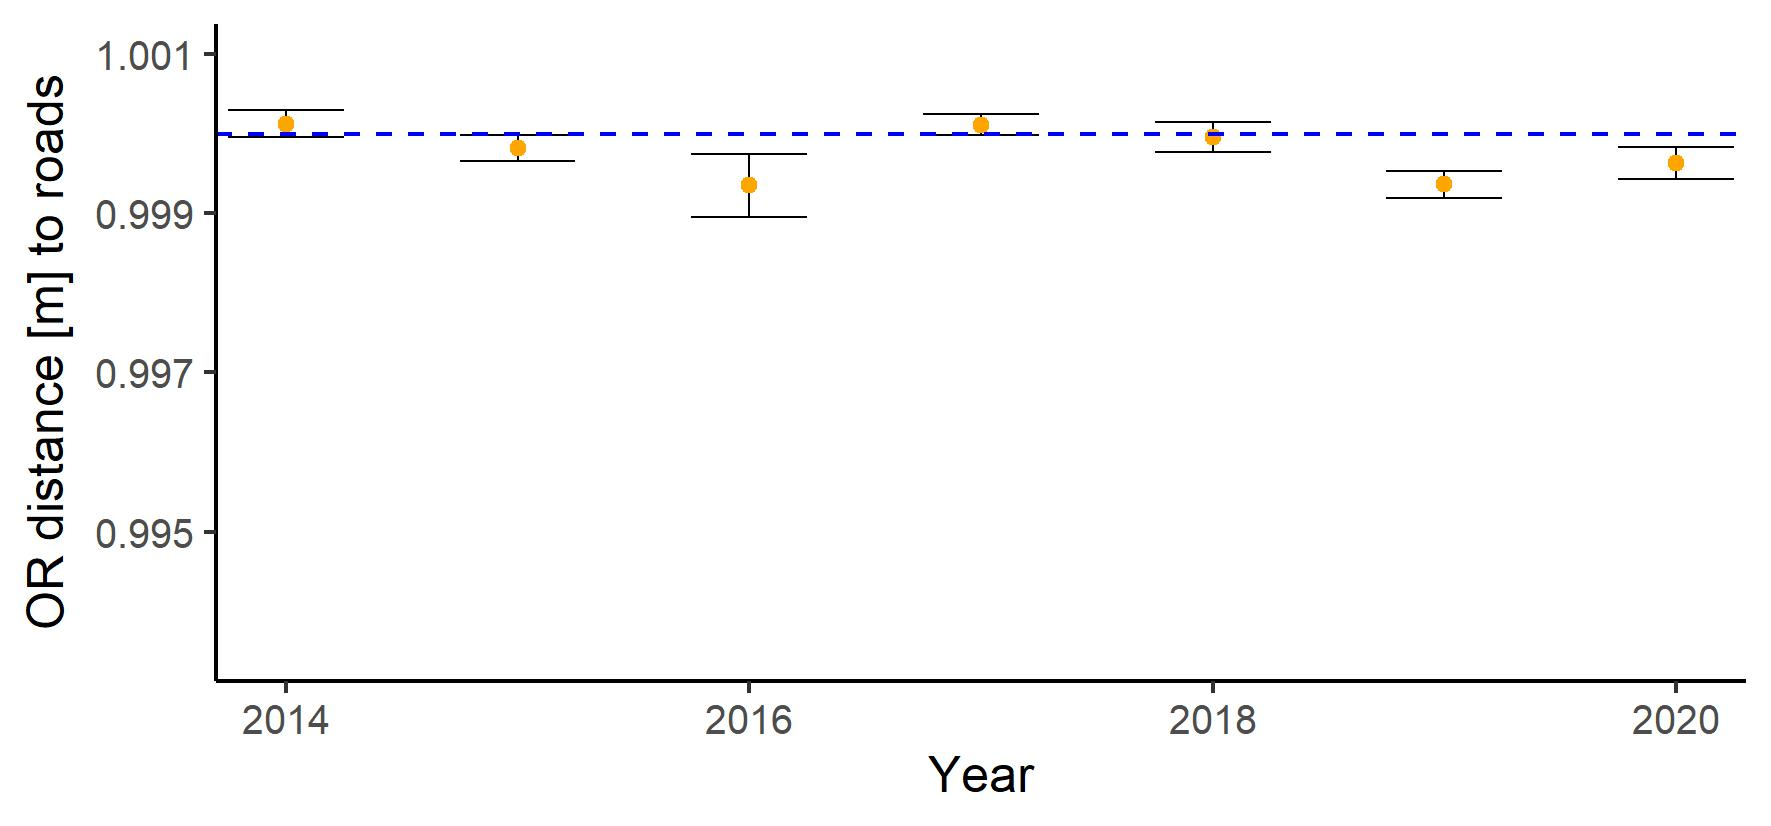
\includegraphics[width = 15 cm]{figures/logreg_year_Roadist.jpeg}
\end{tikzpicture}
\caption{Overall pseudo R$^2$ (Mc Fadden) for the linear regression over each separate year, and the corresponding odds ratios (OR) for the variables distance backfills in the previous year, distance to roads, and distance to impervious surfaces [hm]. The error bars show the 95\% confidence interval of the odds ratio. The boundary of 1 for interpretation and significance of the odds ratios is indicated by the dashed line.}
\label{fig:logitimeseriesBF}
\end{figure}

\iffalse
\begin{figure}[H]
\begin{tikzpicture}
%\node(GEE)at (6cm,-12.75cm)[color=red!80]{R/ R-Studio};
\draw(0, 0.125cm) node[inner sep=0]{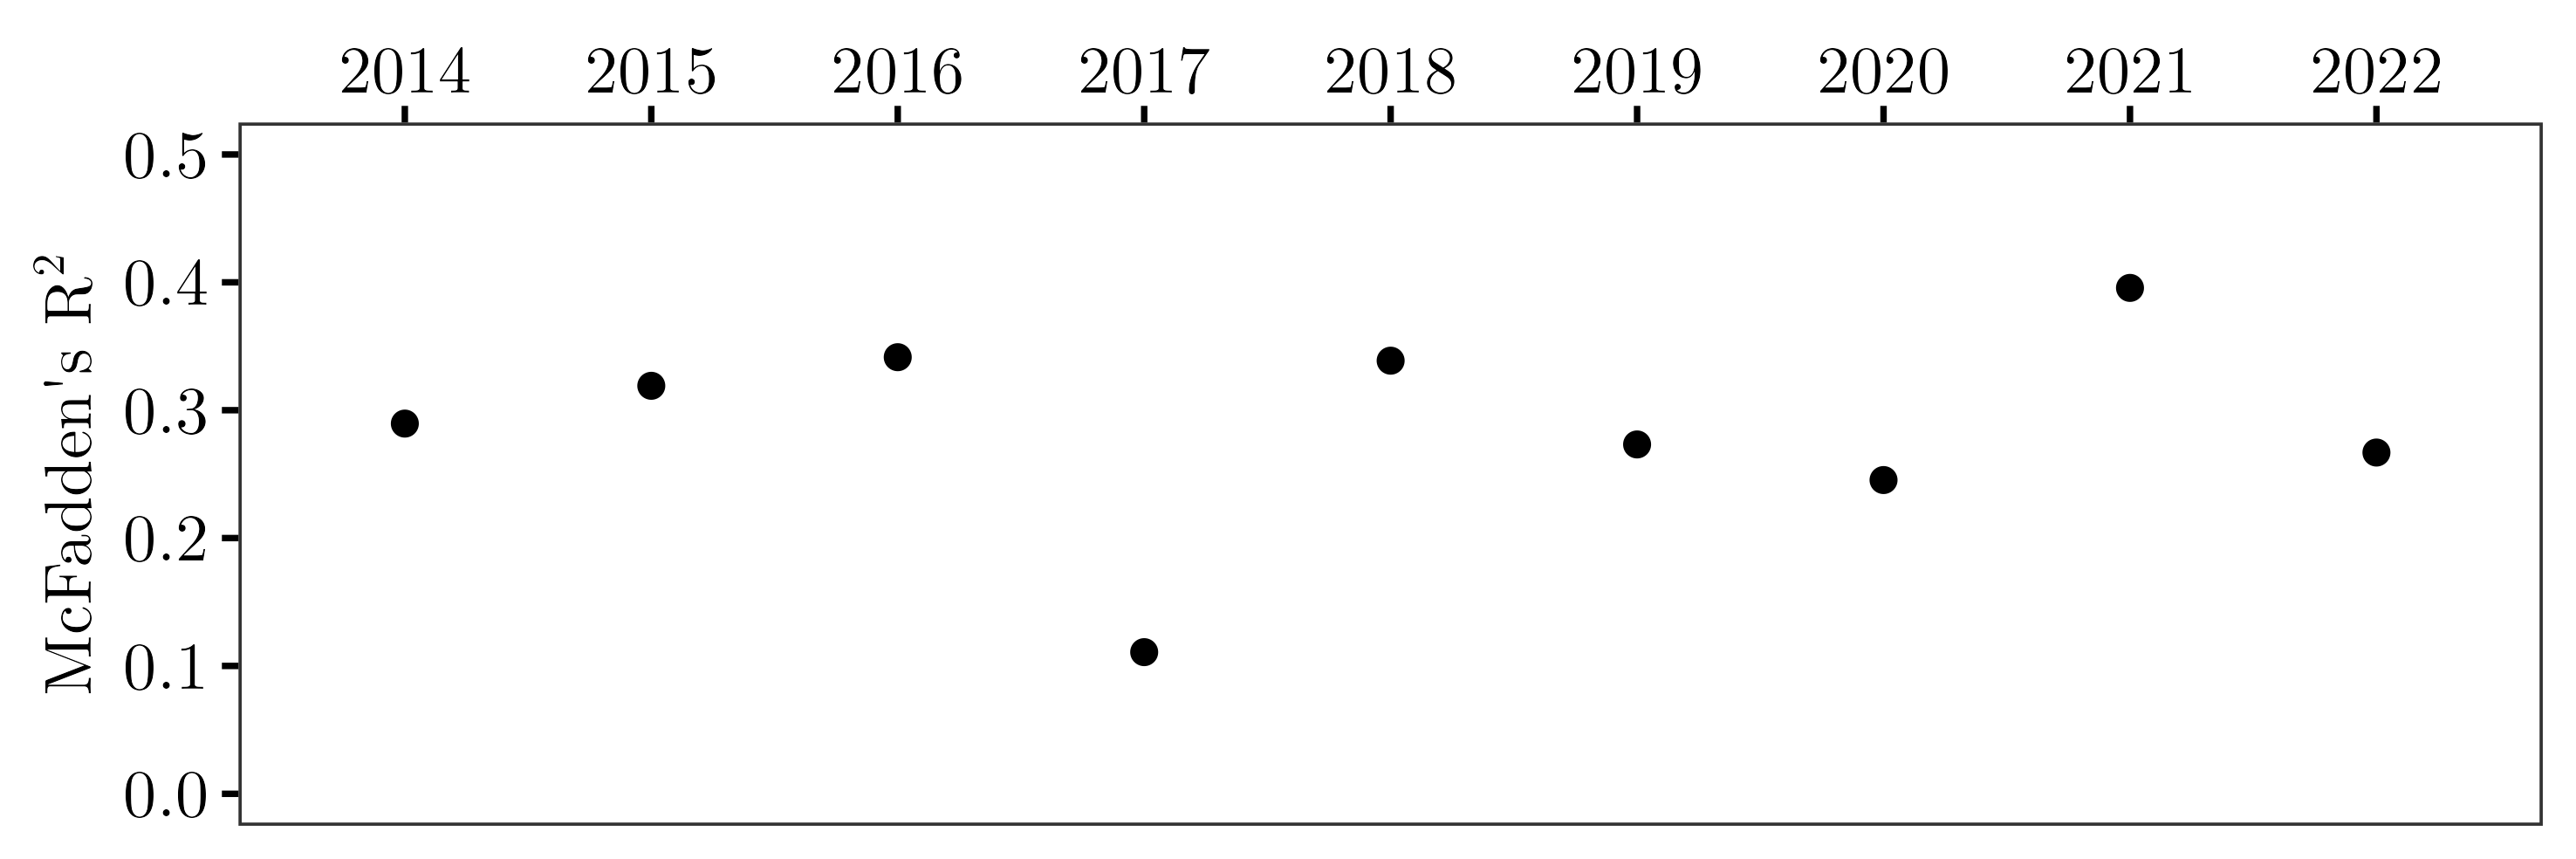
\includegraphics[width = 15 cm]{figures/3_results/logreg_year_Rsq.png}};\\
\node(A)at (-5.75cm,1.625cm)[]{\Large\textbf{A}};

\draw(0, -5.5cm) node[inner sep=0, xshift=0.05cm]{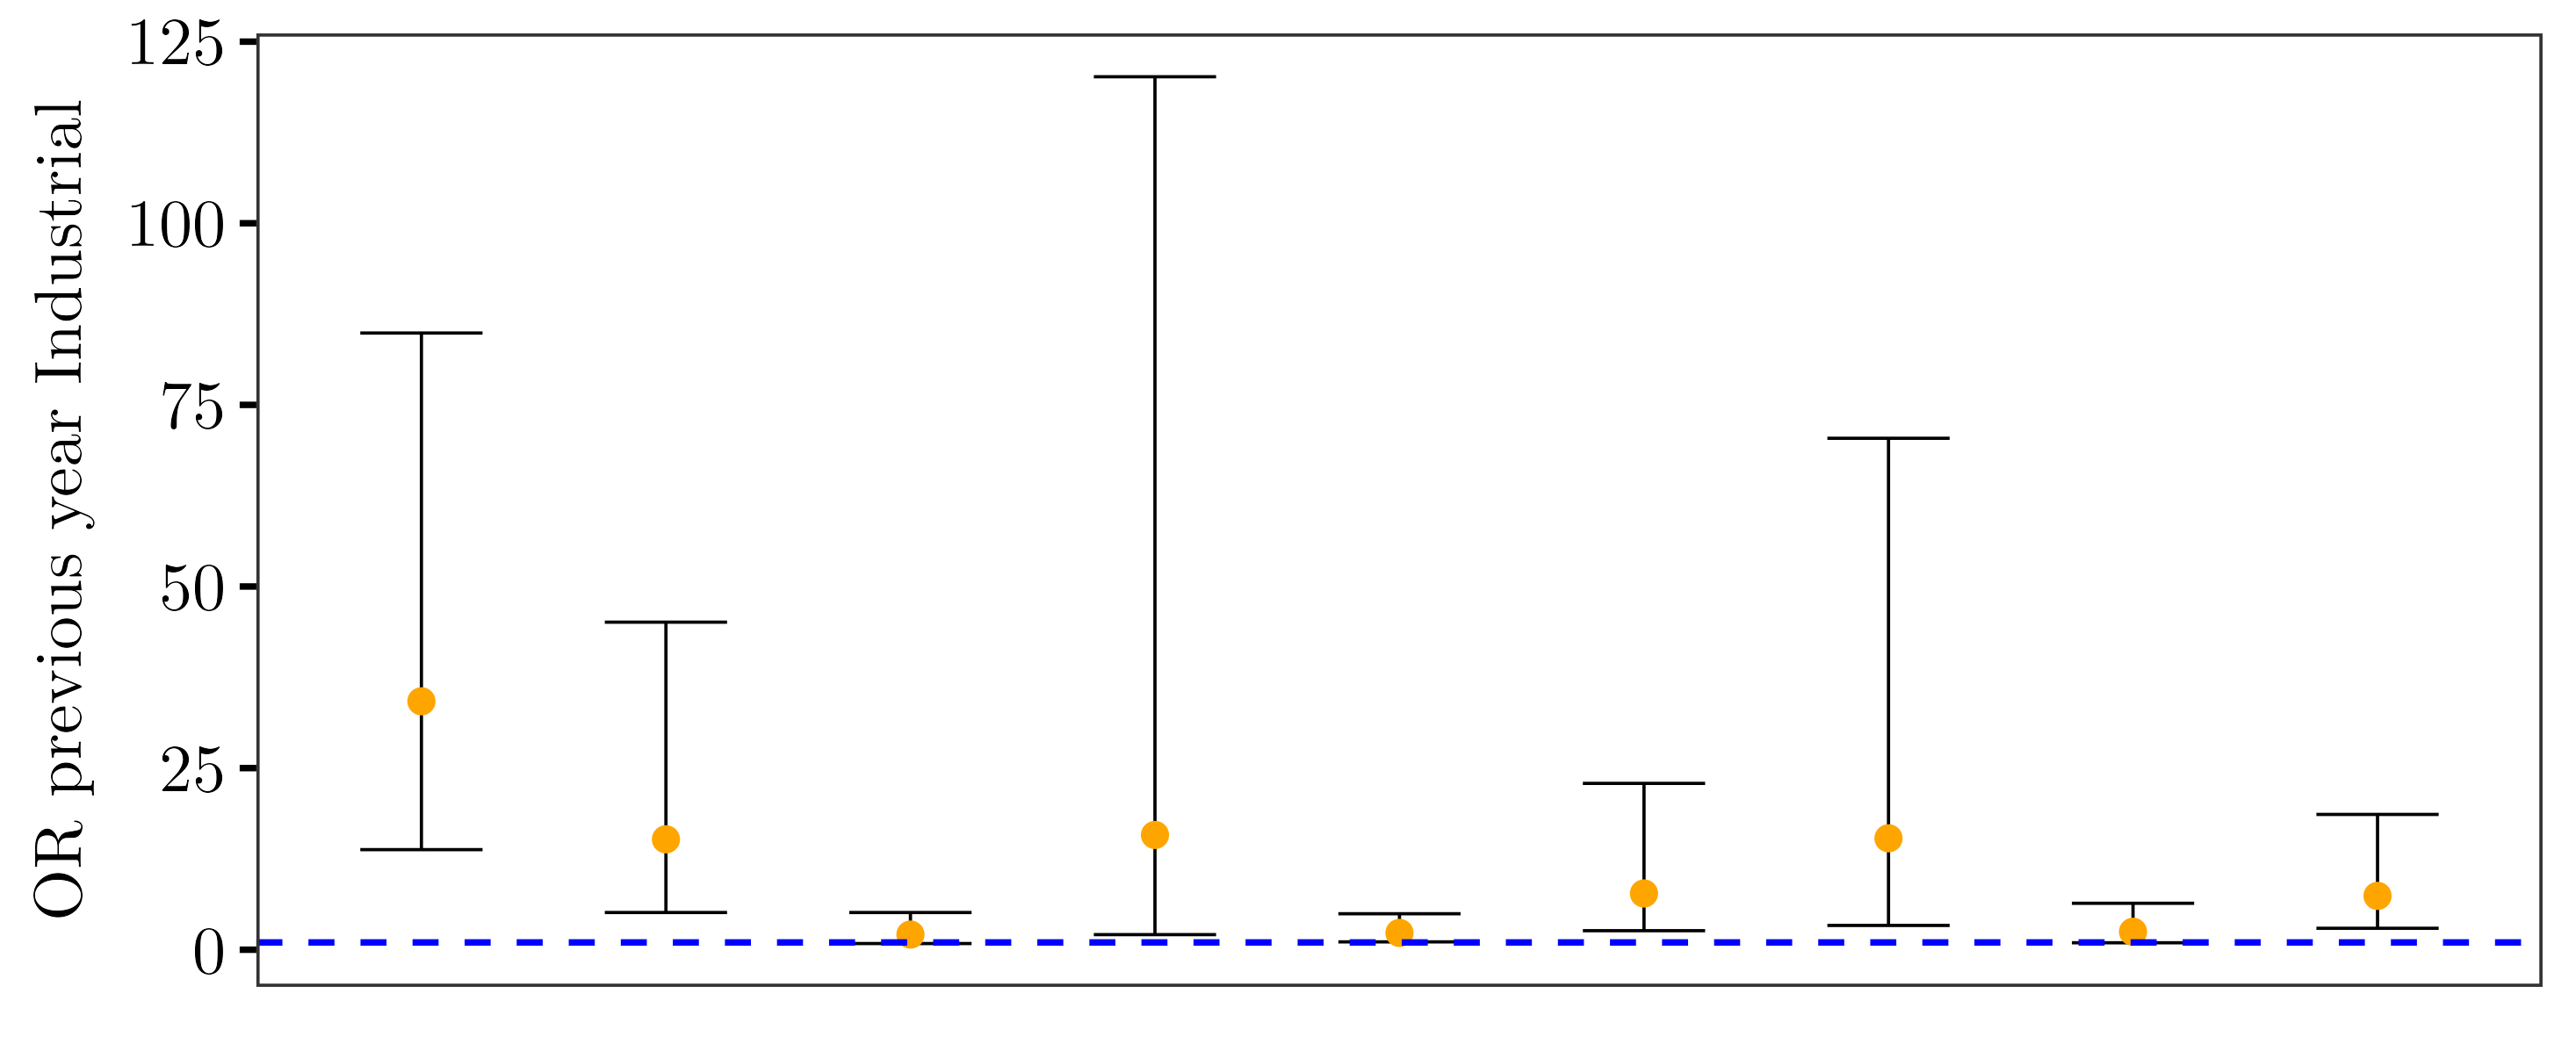
\includegraphics[width = 14.9 cm]{figures/3_results/logreg_year_pycInd.png}};\\
\node(B)at (-5.75cm,-3cm)[]{\Large\textbf{B}};

\draw(0, -12cm) node[inner sep=0]{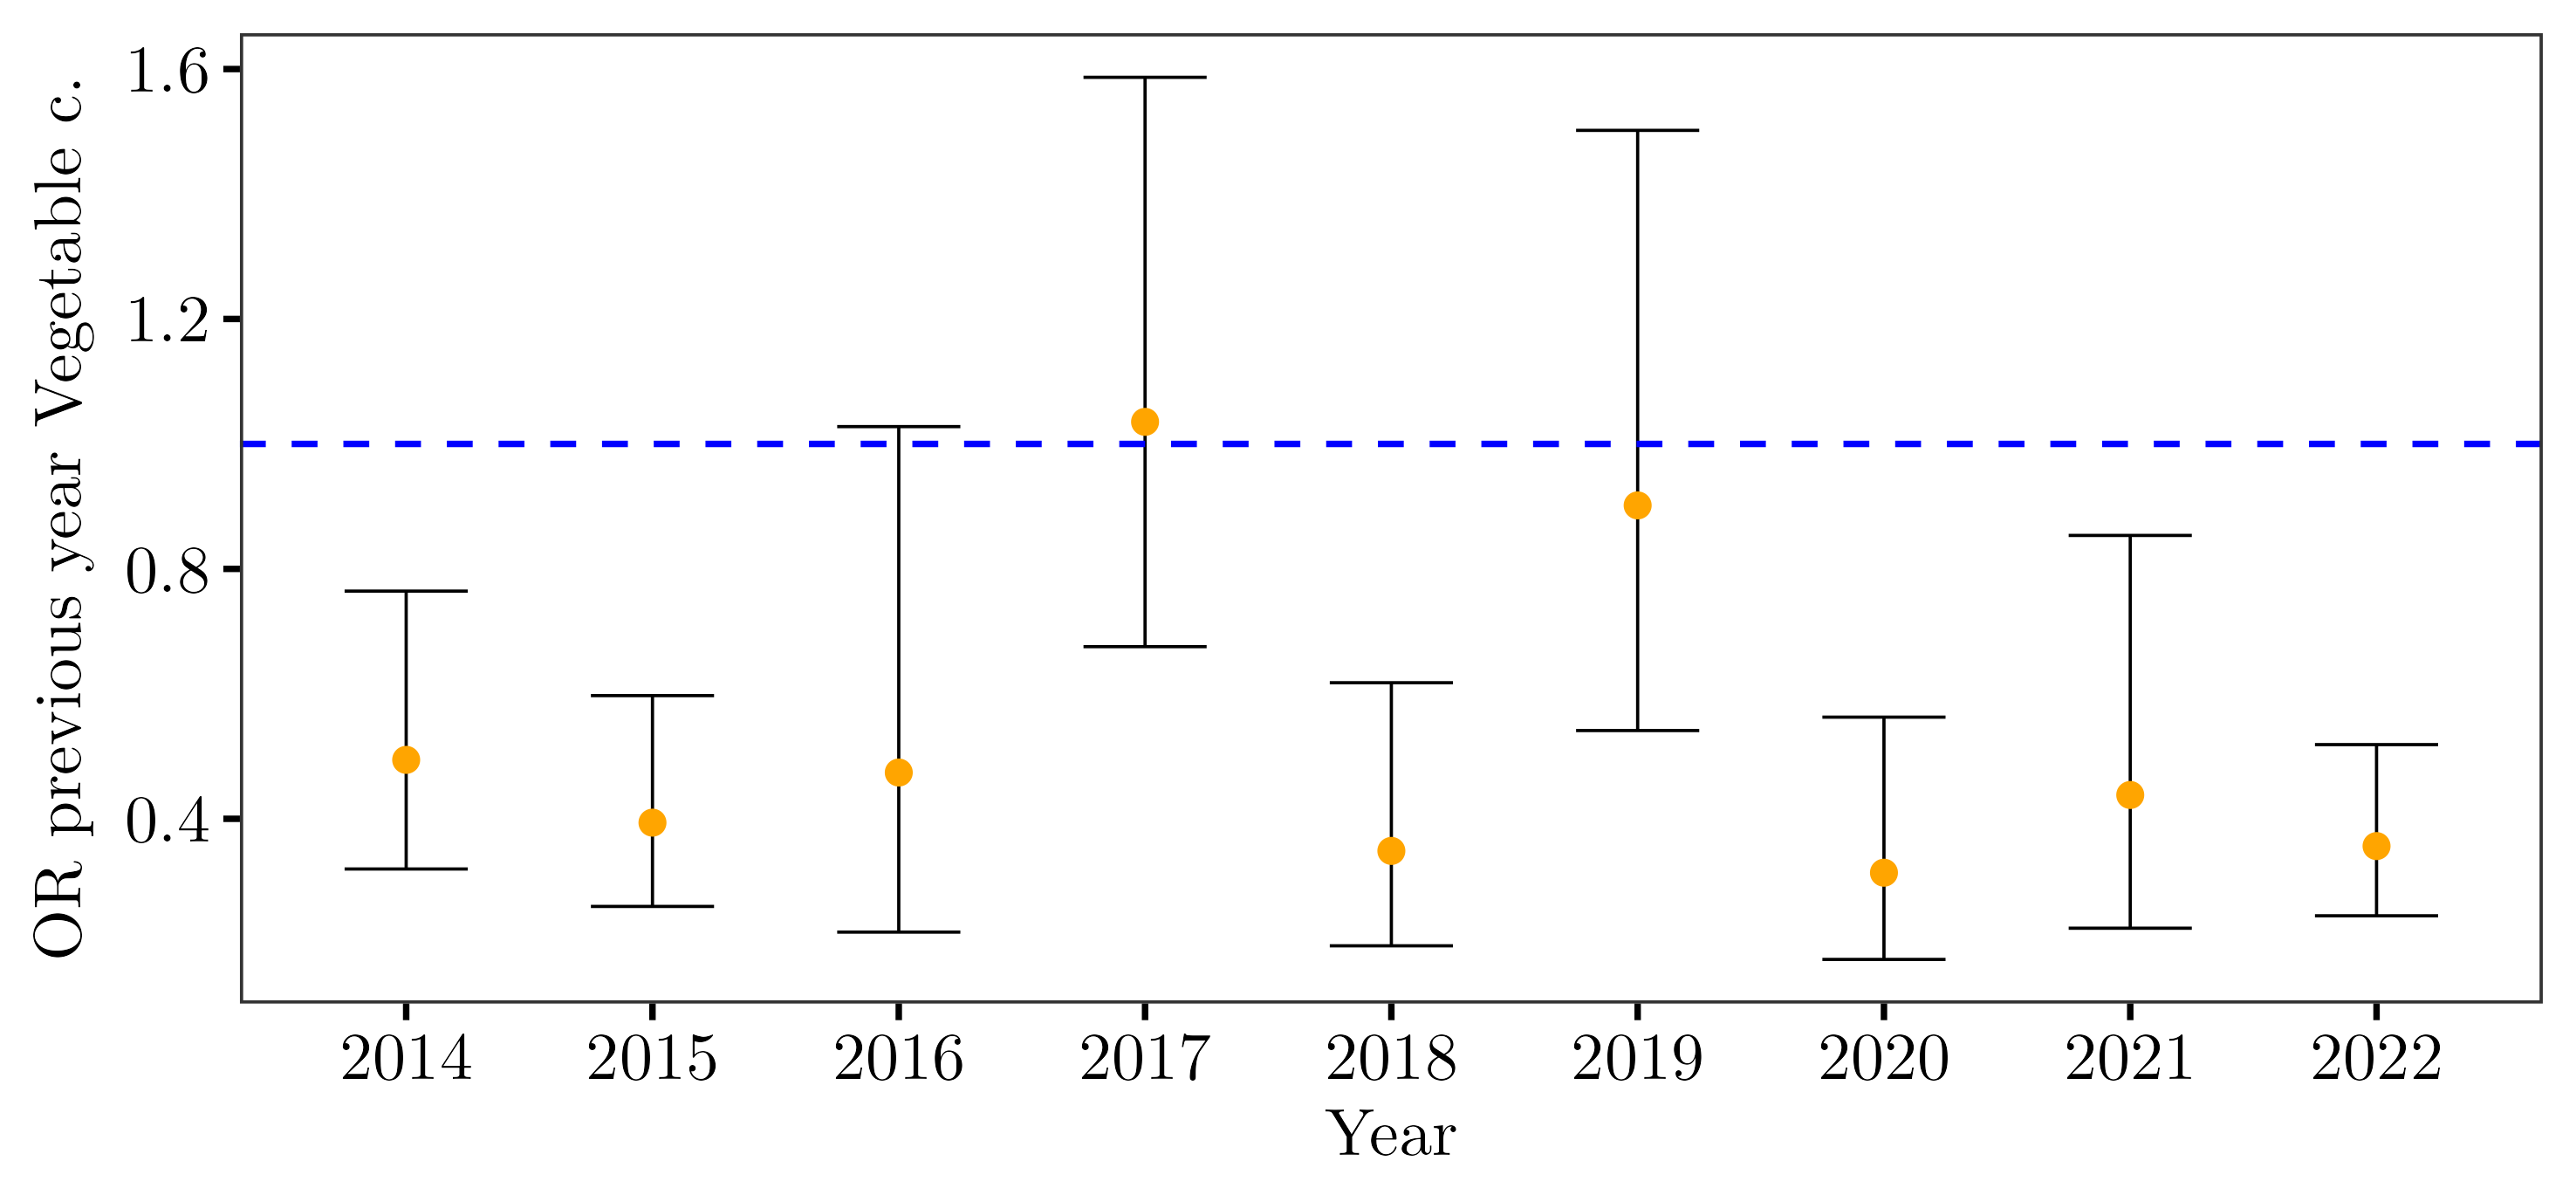
\includegraphics[width=15cm]{figures/3_results/logreg_year_pycVeget.png}};\\
\node(C)at (-5.75cm,-9cm)[]{\Large\textbf{C}};
%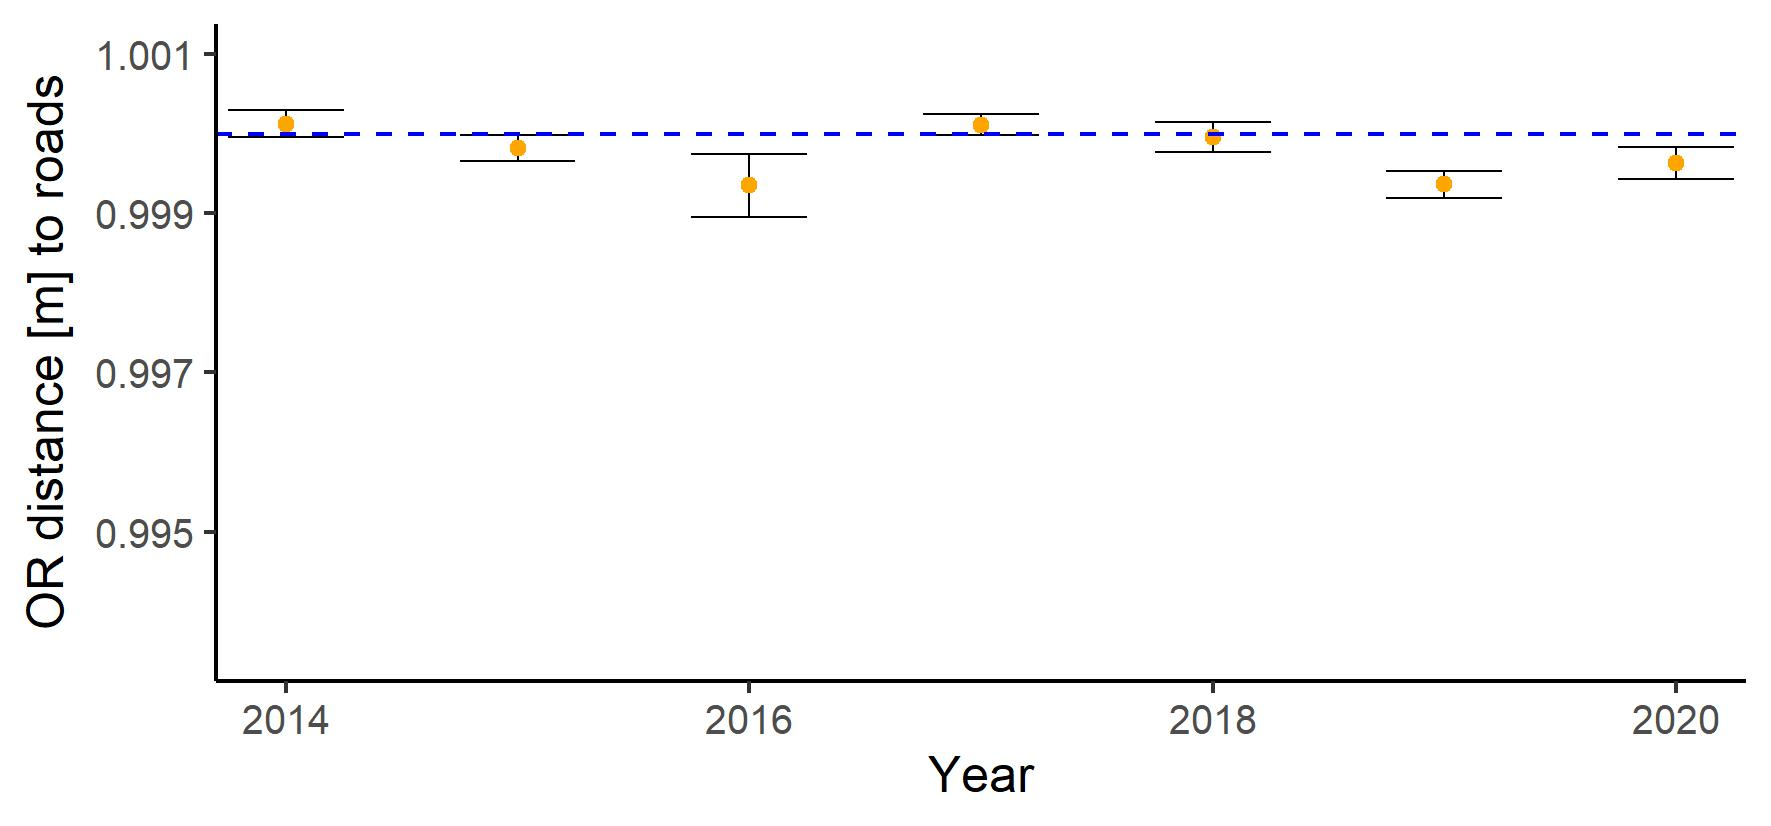
\includegraphics[width = 15 cm]{figures/logreg_year_Roadist.jpeg}
\end{tikzpicture}
\caption{Overall R$^2$ (Mc Fadden) for the linear regression over each separate year, and the corresponding odds ratios (OR) for the variables of the previous year classification as Industrial and Vegetable crop. The error bars show the 95\% confidence interval of the odds ratio.}
\label{fig:logitimeseries}
\end{figure}
\fi

\subsection{Year 2018}
Due to these considerable differences, and the low explanatory value of the model when used for data of all years, we also include the results of one separate year here. Since the overall classification, from which the distance data and previous year classification originate, is only validated for the year 2017, and since there can be strong differences between years (Chapter \ref{chap:supervised_classi}, p. \pageref{chap:supervised_classi}), the results of the regression model for backfill area increase of 2018 are shown. In this data, the classification- and distances to other landcover classes in the previous year are from 2017. For this timestep the model shows a higher fit with a Mc Fadden's pseudo R$^2$ of 0.34.

Boxplots comparing backfills and control data show strong differences, especially for the distance to previous backfills, and also for the distance to impervious areas. The difference is less strong for the distance to roads. Outliers were very abundant for all variables.

The regression model for the 2018 image again shows the highest variable importance for the distance to previous year backfills, and the odds ratio is a lot lower, indicating that the odds of new backfills occurring decreased by 32 \% (OR, 0.68 | 95\% CI [0.643, 0.718]) for a unit [hm] increase in distance to existing backfills in the previous year, assuming that other variables stay constant. In this year, also the distance to impervious areas and industrial areas, and vegetable crop pixels in the year before showed a correlation with backfill distribution, all indicating that backfills had higher odds to occur close to these LULC classes. It strikes the eye that there is a high odds ratio of 2.3 for the previous year classification Industrial variable, indicating that the classification as industrial area in the year before increased the log odds for newly backfilled areas. Previous year classification as crop class, when significant, lowered the log odds of new backfills occurring (Table \ref{tab:logreg18}, p. \pageref{tab:logreg18}).




\begin{figure}[H]
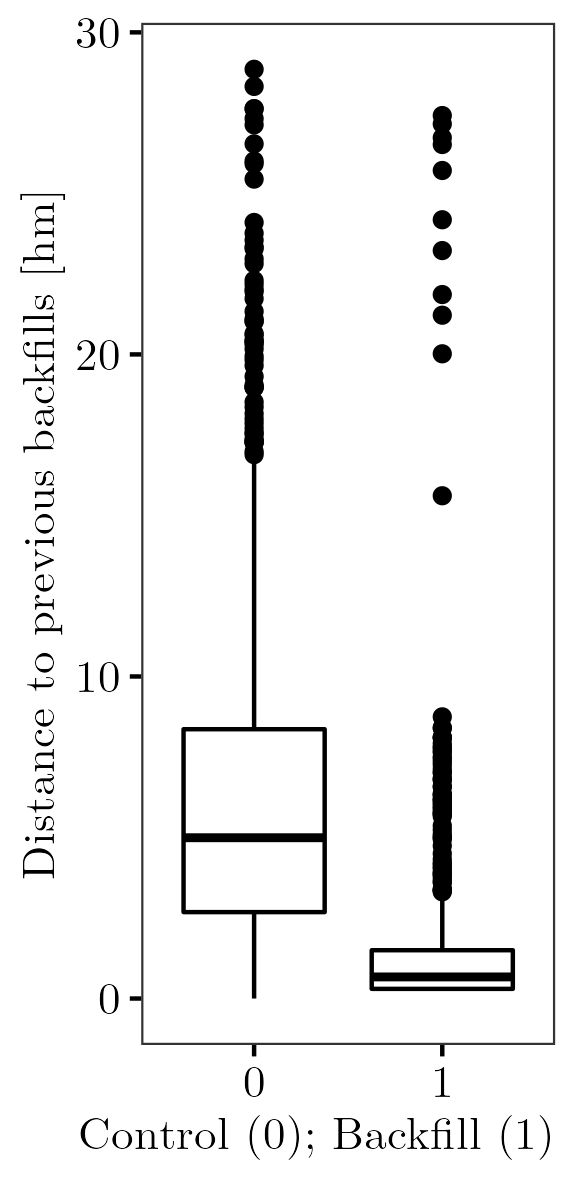
\includegraphics[width = 4.9 cm]{figures/3_results/boxplot backfill logi_18.png}
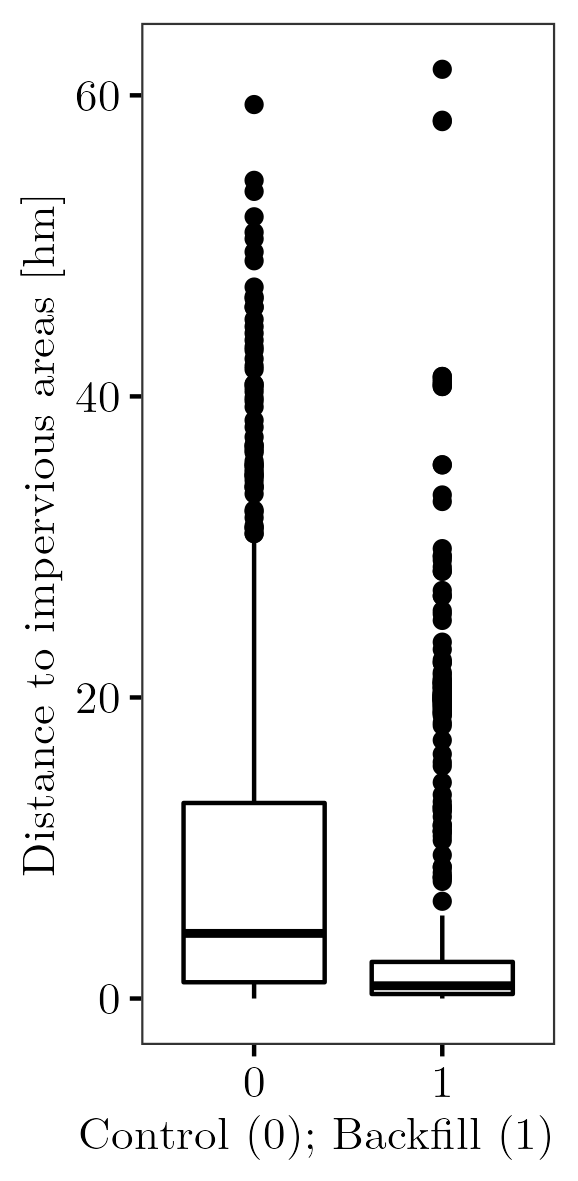
\includegraphics[width = 4.9 cm]{figures/3_results/boxplot imperv logi_18.png}
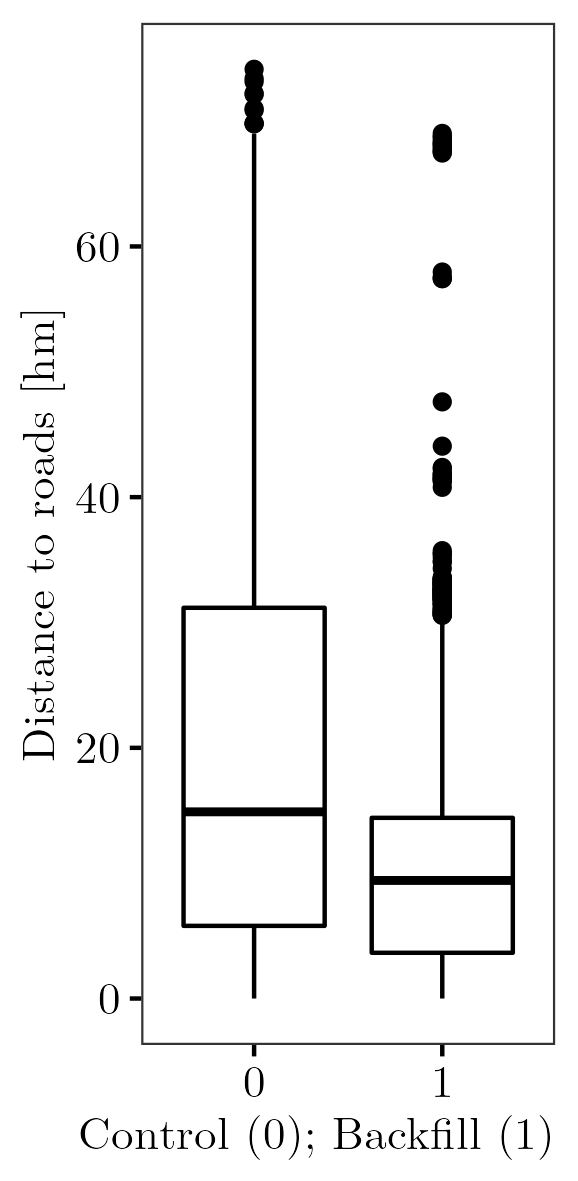
\includegraphics[width = 4.9 cm]{figures/3_results/boxplot roads logi_18.png}
\caption{Comparison of the yearly backfill increments and control with respect to the distance [m] to backfills in the previous year and roads for the year 2018 and distances to other landcovers in 2017.}
\label{fig:logibox_17}
\end{figure}

\begin{table}[ht]
\centering
\caption{Summary of the logistic regression for the year 2018, the previous year being 2017 for which the supervised classification was validated. For all independent variables used, the odds ratio (OR), lower and upper boundaries (Low, Up) of the 95\% confidence interval, variable importance (VI) and the p - value (P) are given. The overall analysis has a pseudo R$^2$ (Mc Fadden) of 0.34.} 
\label{tab:logreg18}
\begin{tabular}{ccccccc}

    \hline
  Unit & Variable & OR & Low & Up & VI & P \\ 
  \hline
\multirow{10}{3cm}{Distance [hm] to land cover in the previous year} 
 & Backfill & 0.68 & 0.643 & 0.718 & 13.8 & *** \\ 
  & Built-up & 1.009 & 0.875 & 1.165 & 0.1 &  \\ 
  & Impervious areas & 0.952 & 0.93 & 0.975 & 4.1 & *** \\ 
  & Industrial & 0.818 & 0.755 & 0.888 & 4.8 & *** \\ 
  & Ricefield & 1.444 & 0.969 & 2.153 & 1.8 & . \\ 
  & Roads & 1.009 & 0.993 & 1.025 & 1.1 &  \\ 
  & Vegetable crop & 0.654 & 0.552 & 0.774 & 4.9 & *** \\ 
  & Water bodies & 1.05 & 1.012 & 1.089 & 2.6 & ** \\ 
  & Watercress & 0.94 & 0.878 & 1.006 & 1.8 & . \\ 
  & Wetland & 0.927 & 0.828 & 1.038 & 1.3 &  \\ 
   \hline
\multirow{6}{3cm}{Previous year classification (factor of 0/1)}
  & Built-up & 1.099 & 0.627 & 1.927 & 0.3 &  \\ 
  & Industrial & 2.311 & 1.079 & 4.951 & 2.2 & * \\ 
  & Ricefield & 1.002 & 0.64 & 1.569 & 0 &  \\ 
  & Vegetable crop & 0.349 & 0.197 & 0.618 & 3.6 & *** \\ 
  & Water bodies & 0.081 & 0.018 & 0.375 & 3.2 & ** \\ 
  & Watercress & 0.27 & 0.132 & 0.551 & 3.6 & *** \\ 
  & Wetland & 0.78 & 0.443 & 1.375 & 0.9 &  \\ 
    \hline
   \multicolumn{7}{c}{p values: \qquad *** < 0.001;\quad ** < 0.01;\quad * < 0.05;\quad . < 0.1 }\\
   \hline
\end{tabular}

\end{table}

\newpage
\chapter{Discussion}
\section{Supervised classification}

\subsection{Validation}
Validated for the year 2017, the supervised classification model delivers results similar to the model from \citet{Dupuy.2020a}, from which the training data was sourced. The overall accuracy and Cohen's Kappa coefficient are close to the values that were estimated for the source model at Level 3 of the class detail (they defined 4 levels of class detail), of which most training classes used in our model originated. They found an overall accuracy of 84\% and a Cohen's Kappa of 0.83 at the classification resolution on Level 3, which is both very close to the accuracy estimates in this thesis (0.84 and Cohen's Kappa 0.82, \cite{Dupuy.2020a}). Thus it can be stated, that for the image composite of 2017, our modified LULC - classification could, for the classes that were taken over, quite well reproduce the original one, although clipping the area to a smaller extent and keeping in mind, that the training data was modified and downsampled. 

In order to best classify backfilled areas, which was the goal in this thesis, it might also be feasible to design a simpler classification model than the one used here. Either by merging existing classes, that can be grouped together, like water bodies and wetlands, or by defining them more broadly in the beginning, potentially collecting ground truth data from high resolution images to train the model.

\subsection{Classification}
As shown in chapter \ref{chap:classifiedmaps} (p. \pageref{chap:classifiedmaps}) The resulting classified images show considerable differences between the years, especially for certain classes. In 2016 this is very clearly visible, since lots of the areas, that are known to consist mainly of rice fields in the plains, were classified as wetland, or even water bodies. This highlights the problem of using training data for only one year over a time series, which in this case caused varying classification results. In a future attempt it might be useful, to create a more elaborate set of training data with respect to using data from different years. In our case, the polygons were only used to gather training data for the image 2017, since the collection of ground truth data took place over the 2017 rainy season (\cite{Dupuy.2020a, Dupuy.2020b}). The Figure \ref{fig:Rt_franco} illustrates, that backfills for roads were prevalent and also identified by the model, despite the road sometimes already being built over on the image acquisition date.


\section{Backfill area increase}
\subsection{Validation}
The validation of backfill classifications was done, to estimate the accuracy of the backfill classifications in the training year (2017) and two additional years (2013 and 2018), to get an idea of how well backfills are identified over the time series. The dataset that was acquired by expert analyses of a list of areas that had been identified as backfill in a preliminary stage of the classification model, shows that the larger fraction of the areas of the backfill class were accurately classified. There are strong differences between the years. One problem is, that in all years there was more reference data on backfills, than on other areas. This infers a lack of control data, potentially causing bias, especially for the accuracy of areas that were estimated to not be backfilled. In the years 2013 and 2021 this is a problem, with the fraction of areas falsely classified as backfills being high in both cases (90 \% and 42 \% respectively), compared to all areas that are known to not be backfilled. For both years, this could show a tendency of the classification model to overpredict backfilled areas, yet this statement would be stronger with more balanced data. The mean accuracy of backfill recognitions in the years 2013 and 2021 is in the same range as the overall accuracy of the classification model for the year 2017, whereas the Cohen's Kappa value is very low. The low Cohen's Kappa is explained by the strong imbalance of the dataset in combination with many falsely identified areas, compared to the total number of samples that are not backfills. It can be argued that this accuracy estimate is not the most suitable in such a case, since the focus of the analyses lies on the class of backfill, more than on the others. In this case, the measure of user's accuracy (mean = 0.88) for the backfill class should be more fitting, indicating the share of correctly classified backfills in all areas classified as backfills (\cite{Olofsson.2014, Strahler.2006}).

%2013 being the only image that is not a composite/ cloudmasked due to lack of enough images might also play a role in bf classification being worse in this year
\subsection{Time-series}
%roads -->maybe linking road constructions to high values also useful for regression
What stands out in the area increase data, is the relatively high value for the year 2017  and the relatively low values for 2016 and 2021 (Figure \ref{fig:areakm2}, p. \pageref{fig:areakm2}). As mentioned in chapter \ref{chap:classifiedmaps} (p. \pageref{chap:classifiedmaps}), parts of the building of two new roads, which had to be filled up first, since they lead through the rice plains surrounding Antananarivo,  took place over the course of 2016. Both of these were in parts classified as backfills in the 2017 classification, since the raised soil was still prevalent then. These roads and the largest backfilled area found in this study (to the north of the city), which grew considerably between the imaging dates of 2016 and 2017 made up for approximately 0.82 km$^2$ of the area increase in this year, explaining the high backfill increase value calculated for 2017 (Figures \ref{fig:cls16} and \ref{fig:cls17} on pp. \pageref{fig:cls16} - \pageref{fig:cls17} for the respective maps). Possible reasons for the low values in 2016 and 2021 are a bit harder to estimate, since there are no visual clues on the maps themselves. %area value calculated in ArcGis

There is the question on if, or how political actions and actors could influence the backfill activity in a year. In January of 2014, Hery Rajaonarimampianina was sworn in as president following the elections.
In January of 2019 Andry Rajoelina won the presidential election (\cite{BBC.2018}). In both cases the backfill increase data (Figure \ref{fig:areakm2}) shows a small dip in the year after and a stronger dip two years after. This might hint at an impact of new legislation (or plans for it) in the beginning of both presidential periods. In both cases this was subsequently followed by a relatively high value of yearly backfill increase, especially for 2017. Prevalent from postings in the media about new legislation and its impact, and also from the yearly area increments established here, it does not make the impression, that legislation or bans from backfilling currently hinder the process sustainably.
%mention the importance of industrial area and of visual inspection of the increase map
%Comparison to the timeseries of major events by Constance.


%
The mean increase in backfilled area is low, considering the size of the study area, This also led to the low conversion rate from BGI to backfill, which would ultimately become urban or built-up land to be low. %comparison to other landcover changes, optimally in the region%
%\textbf{Laurence Defrise} found that in Antananarivo the increase of urban %land is not as high, as in other cities, which is supported by our findings %of a low rate of backfilling.

%why is the issue controversial if the impact is so small? -->maybe its the otehr way around and the impact is small, because it is controversial

%in future it might be interesting to get infomation on how long backfills normally stay barren



%Comparison to other landcover changes
\subsection{Backfill size distribution}
The size distribution of backfilled areas indicates, that there are more small backfills than large ones.  It is debatable, whether this means that they also have a higher impact on yearly backfill area increase. Especially very small values below 0.1 ha have to be considered with caution, since these account for only one pixel. On this scale, a lot of inaccuracies were observed on the classified- and backfill increase maps. Another potential error is that long backfills (like roads) often had interrupts of more than one missing pixels, meaning that they would have been defined as two or more separate areas. Thus, it makes sense to have a look if this relationship also holds up for backfills of a bit larger scale. When looking at backfilled areas of an arbitrary size of 0.5 ha and larger, it becomes clear that the smaller ones can also account for a considerable part of the area increase overall. For instance, looking at 40 backfills of one hectare area compared to two backfills of 10 hectares. However, this relationship is not as extreme, as it seems when looking at very small classified backfill pixels. It is also plausible, that in specific years with a large backfill area increase, a few large areas make up for the most of it, as was the case when looking at the classification for 2017

%*comparere to backfill typologies described by aubrieu et al.

\section{Drivers of backfilling} 
\subsection{All years}
In all yearly intervals the regression showed, that the distance to backfills in the year before was the most important, and influential independent variable. This is consistent with the hypothesis that backfills often occur around other backfills. For the expected behavior of backfills occurring close to urban areas, the results are weaker. The comparison between years shows, that a potential reason for this is high variability between years in terms of model fit and also the predictive power of the odds ratios. Two main hypotheses arise from this: 
\begin{itemize}
\item There are expected to be other variables, having an important relationship to the distribution of backfills in the plains surrounding Antananarivo.

\item Since it is clear, that the model used here fits some yearly time steps quite well, while others barely, and this is in no clear relation to the calculated backfill area increase per year, it is hypothesized, that this difference could stem from various kinds of backfills having different influential factors. Like for instance roads compared to smaller backfills on one plot of land, or large industrial backfills that grow over multiple years.
\end{itemize}

\subsection{Year 2018}
In this year especially, the hypotheis seems to hold up, with a clear importance of the distance to the previous year backfill and built-up classes. The distance to roads is significant and meaningful for the model, yet not in the way expected. The odds' ratio above one, meaning an increase in probability for backfill with increasing unit distance to roads. This could well be due to the fact, that only primary and secondary roads were used in the regression. Small roads were not considered, since it was necessary to adjust the road dataset to the yearly time steps, checking if roads were already around in any given rainy season, and either researching their building date or deriving it visually in Google Earth, which would have taken too much time on a larger dataset of roads. Revisiting this, it would probably still make sense to consider smaller roads in some way.
%further investigationconcerning socoeconomic independent variables like land zoning, prices, ownership etc. might be iinsightful for driver and prediction analyses

%from aubrieu 2011
Defining key variables of backfilling, \citet{Abrieu.2011} states that the most favorable places to be backfilled are defined by the presence of a road, the proximity of an urbanized area, the existence of a construction hub and the quality of life of a neighborhood. The results of the regression analyses align somewhat with proximity to urbanized areas (impervious surfaces) increasing the log odds for new backfills in certain years (as also in 2018). The difference to roads was far less important, than expected. It is hypothesized that is to a large extent due to the usage of a coarse road network in the regression analyses (primary and secondary roads), whereas from a point of view of accessibility almost any road would suffice. In a future attempt, it would be worth considering this. Possibly focussing the analyses with respect to roads on one or a few specific years, since modifying a detailed road dataset to fit a time-series would be very laborious. Using a road dataset that is recent for years in the past is not advised, due to the potential of interference with backfills for roads. This was experienced in our analyses, falsely leading to a higher explanatory value in early regression attempts, because backfills for new roads were compared to datasets which already contained these exact roads.


\chapter{Conclusion}

Supervised random forest classification was found to be an adequate measure to follow and quantify the process of backfilling. Classifying Landsat 8 data at a 30$*$m resolution, could reliably identify such areas. Key factors of the image acquisition, such as temporal interval, specific date, quality of the collection, and the spatial resolution necessary should be carefully considered. The use of Google Earth Engine for the analyses was practical due to the rapid availability of Remotely sensed data. Revisiting the choice of input data for the classification, it is advised to choose various sources, such as spectral data and digital elevation data, since this was observed to have a beneficial impact on the classification. When using supervised classification to identify one class especially, it was useful to incorporate external, already existing training data. In a future attempt it is suggested to thematically merge related classes, and classes that are not of core importance for the research question, in order to enhance the simplicity of the model. It is expected to be beneficial, if not necessary, to acquire training data for multiple years within the time-period of the analyses. This could also be done by customizing the existing data to other years, verifying the classes with high resolution imagery, if available.

Although no explicit expectation was held, the identified yearly increases in backfilled area were found to be lower than anticipated. During the observed time-period, rice fields and other BGI surrounding Antananarivo were not at high risk of being backfilled, although the process was steadily going on, especially in certain regions. Smaller backfilled areas of around 0.5 hectares as well as larger areas of up to 30 hectares are both found to be important in contributing to the yearly increase in backfilled area. The smaller ones accounting for the steady increase- and larger areas for specific peaks in backfilled area. The analysis emphasizes the difference between types of backfilled areas. One factor to be considered here is size. Another important factor was the backfilling to build roads for better connection of the city of Antananarivo and its outskirts or to the Ivato airport. Turnover time differed very strongly here: The identified backfills for roads were built over fast, at times in the same year as backfilling took place, whilest other, especially very large backfills could be observed to stay barren over the whole time series. Yet other backfills progressed steadily, whilst also being built over, e.g.in industrial areas.
%conversion rate somewhere
%the rate of backfilling at the expense of was on average. which is low compared to other LULC changes and in the light of fast uranisation
%typology backill differences

New backfills were found to be most strongly correlated with the distance to already existing ones. Other variables, like distance to roads and built up surfaces, unexpectedly, were not found to be strongly associated. This is inconsistent with known factors of importance for backfilling, such as accessibility (roads), and probably stems from the rather coarse resolution concerning the road network in the analyses. The logistic regression could show some other interesting relationships, like potentially an association with industrial and impervious areas, yet these were not as strong as expected. For a future model of this sort, it would be beneficial to incorporate a finer road network and possibly other third party data, since the overall classification results used for other landcover classes are of questionable reliability in these analyses.
%drivers existing backfill prob roads --> problem of too small road dataset

The urbanization in Antananarivo, based on the remote sensing analyses of backfilled areas, is steadily expanding the city toward it's green outskirts, largely at the expense of BGI. 67.5 \% of newly occurred backfills in the study area were classified as BGI a year before. This sort of expansion increases flood risk, both due to a loss of protection function of the previous landcover, and also due to more vulnerable infrastructure occupying frequently flooded areas. Considering the already large, and potentially growing problem of recurring floods, this is a risky endeavor. Yet a comparably low rate of increase in recognized backfilled areas can give perspective. With awareness and sustainable planning, to which findings of analyses such as this should contribute, a large fraction of this important blue and green infrastructure could be preserved or incorporated in multifunctional landscapes, thus maintaining the city of Antananarivo's resilience in the future.


%%\chapter*{Bibliography}
\newpage
\phantomsection\addcontentsline{toc}{chapter}{Bibliography}
\emergencystretch=1em
\printbibliography


\newpage
\phantomsection\addcontentsline{toc}{chapter}{Appendix}
\chapter*{Appendix}
\section*{Appendix A}
Backfill  area increase in square kilometers in the study area. For both downsampled-, and full training data (TD).
\begin{table}[ht]
\centering
\caption{Backfill area increase per year [km$^2$] in the study area around Antananarivo. all TD = using all training data, ds TD = using downsampled training data.} 
\begin{tabular}{ccc}
  \hline
Backfill increase & Year & training data \\ 
  \hline
0.61 & 2014.00 & all TD \\ 
  0.72 & 2015.00 & all TD \\ 
  0.16 & 2016.00 & all TD \\ 
  1.54 & 2017.00 & all TD \\ 
  0.55 & 2018.00 & all TD \\ 
  0.75 & 2019.00 & all TD \\ 
  0.64 & 2020.00 & all TD \\ 
  0.30 & 2021.00 & all TD \\ 
  0.88 & 2022.00 & all TD \\ 
  0.80 & 2014.00 & ds TD \\ 
  0.68 & 2015.00 & ds TD \\ 
  0.18 & 2016.00 & ds TD \\ 
  1.81 & 2017.00 & ds TD \\ 
  0.59 & 2018.00 & ds TD \\ 
  0.83 & 2019.00 & ds TD \\ 
  0.72 & 2020.00 & ds TD \\ 
  0.27 & 2021.00 & ds TD \\ 
  0.93 & 2022.00 & ds TD \\ 
   \hline
\end{tabular}

\end{table}

\section*{Appendix B, pp. 39 - 45}
Classified maps resulting from the supervised classification
\section*{Appendix C, pp. 46 - 47}
Maps of backfill area increase per year between 2013 and 2022 in Antananarivo.


\begin{figure}[H]
    \centering
    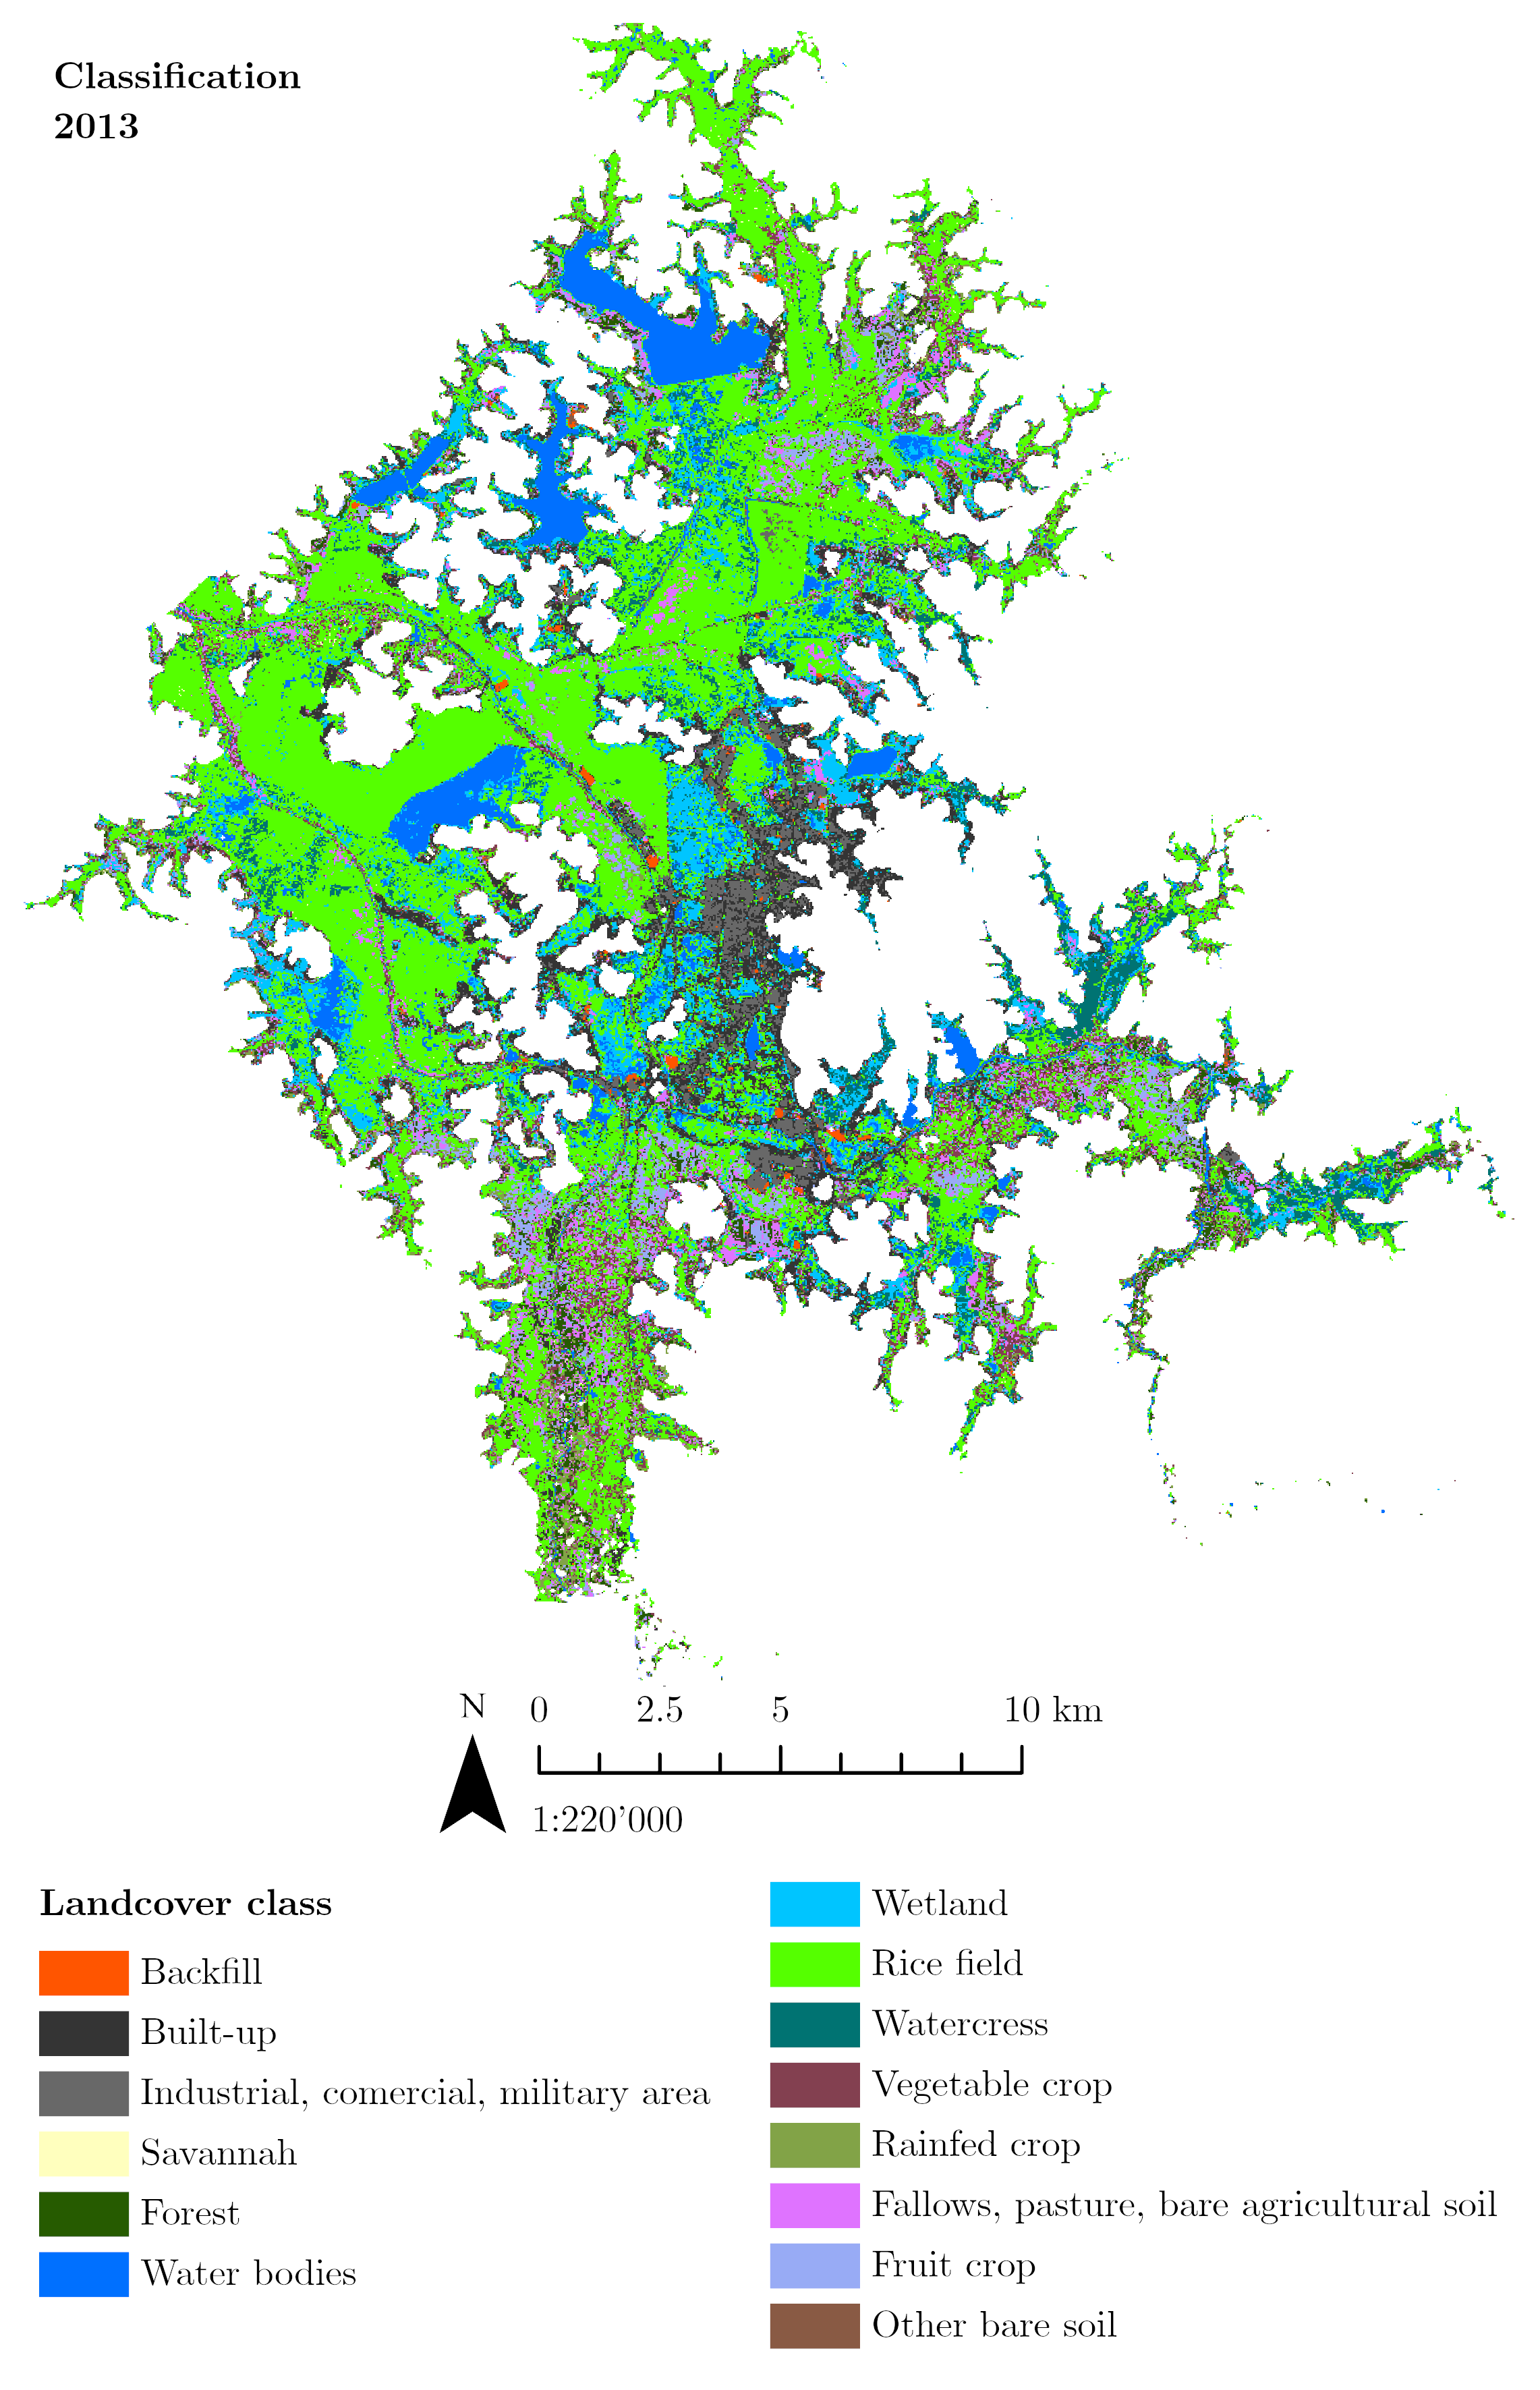
\includegraphics[width = 15cm]{figures/classi2013.png}
    \caption{Classified image resulting from the 2013 classification.}
    \label{}
\end{figure}

\begin{figure}[H]
    \centering
    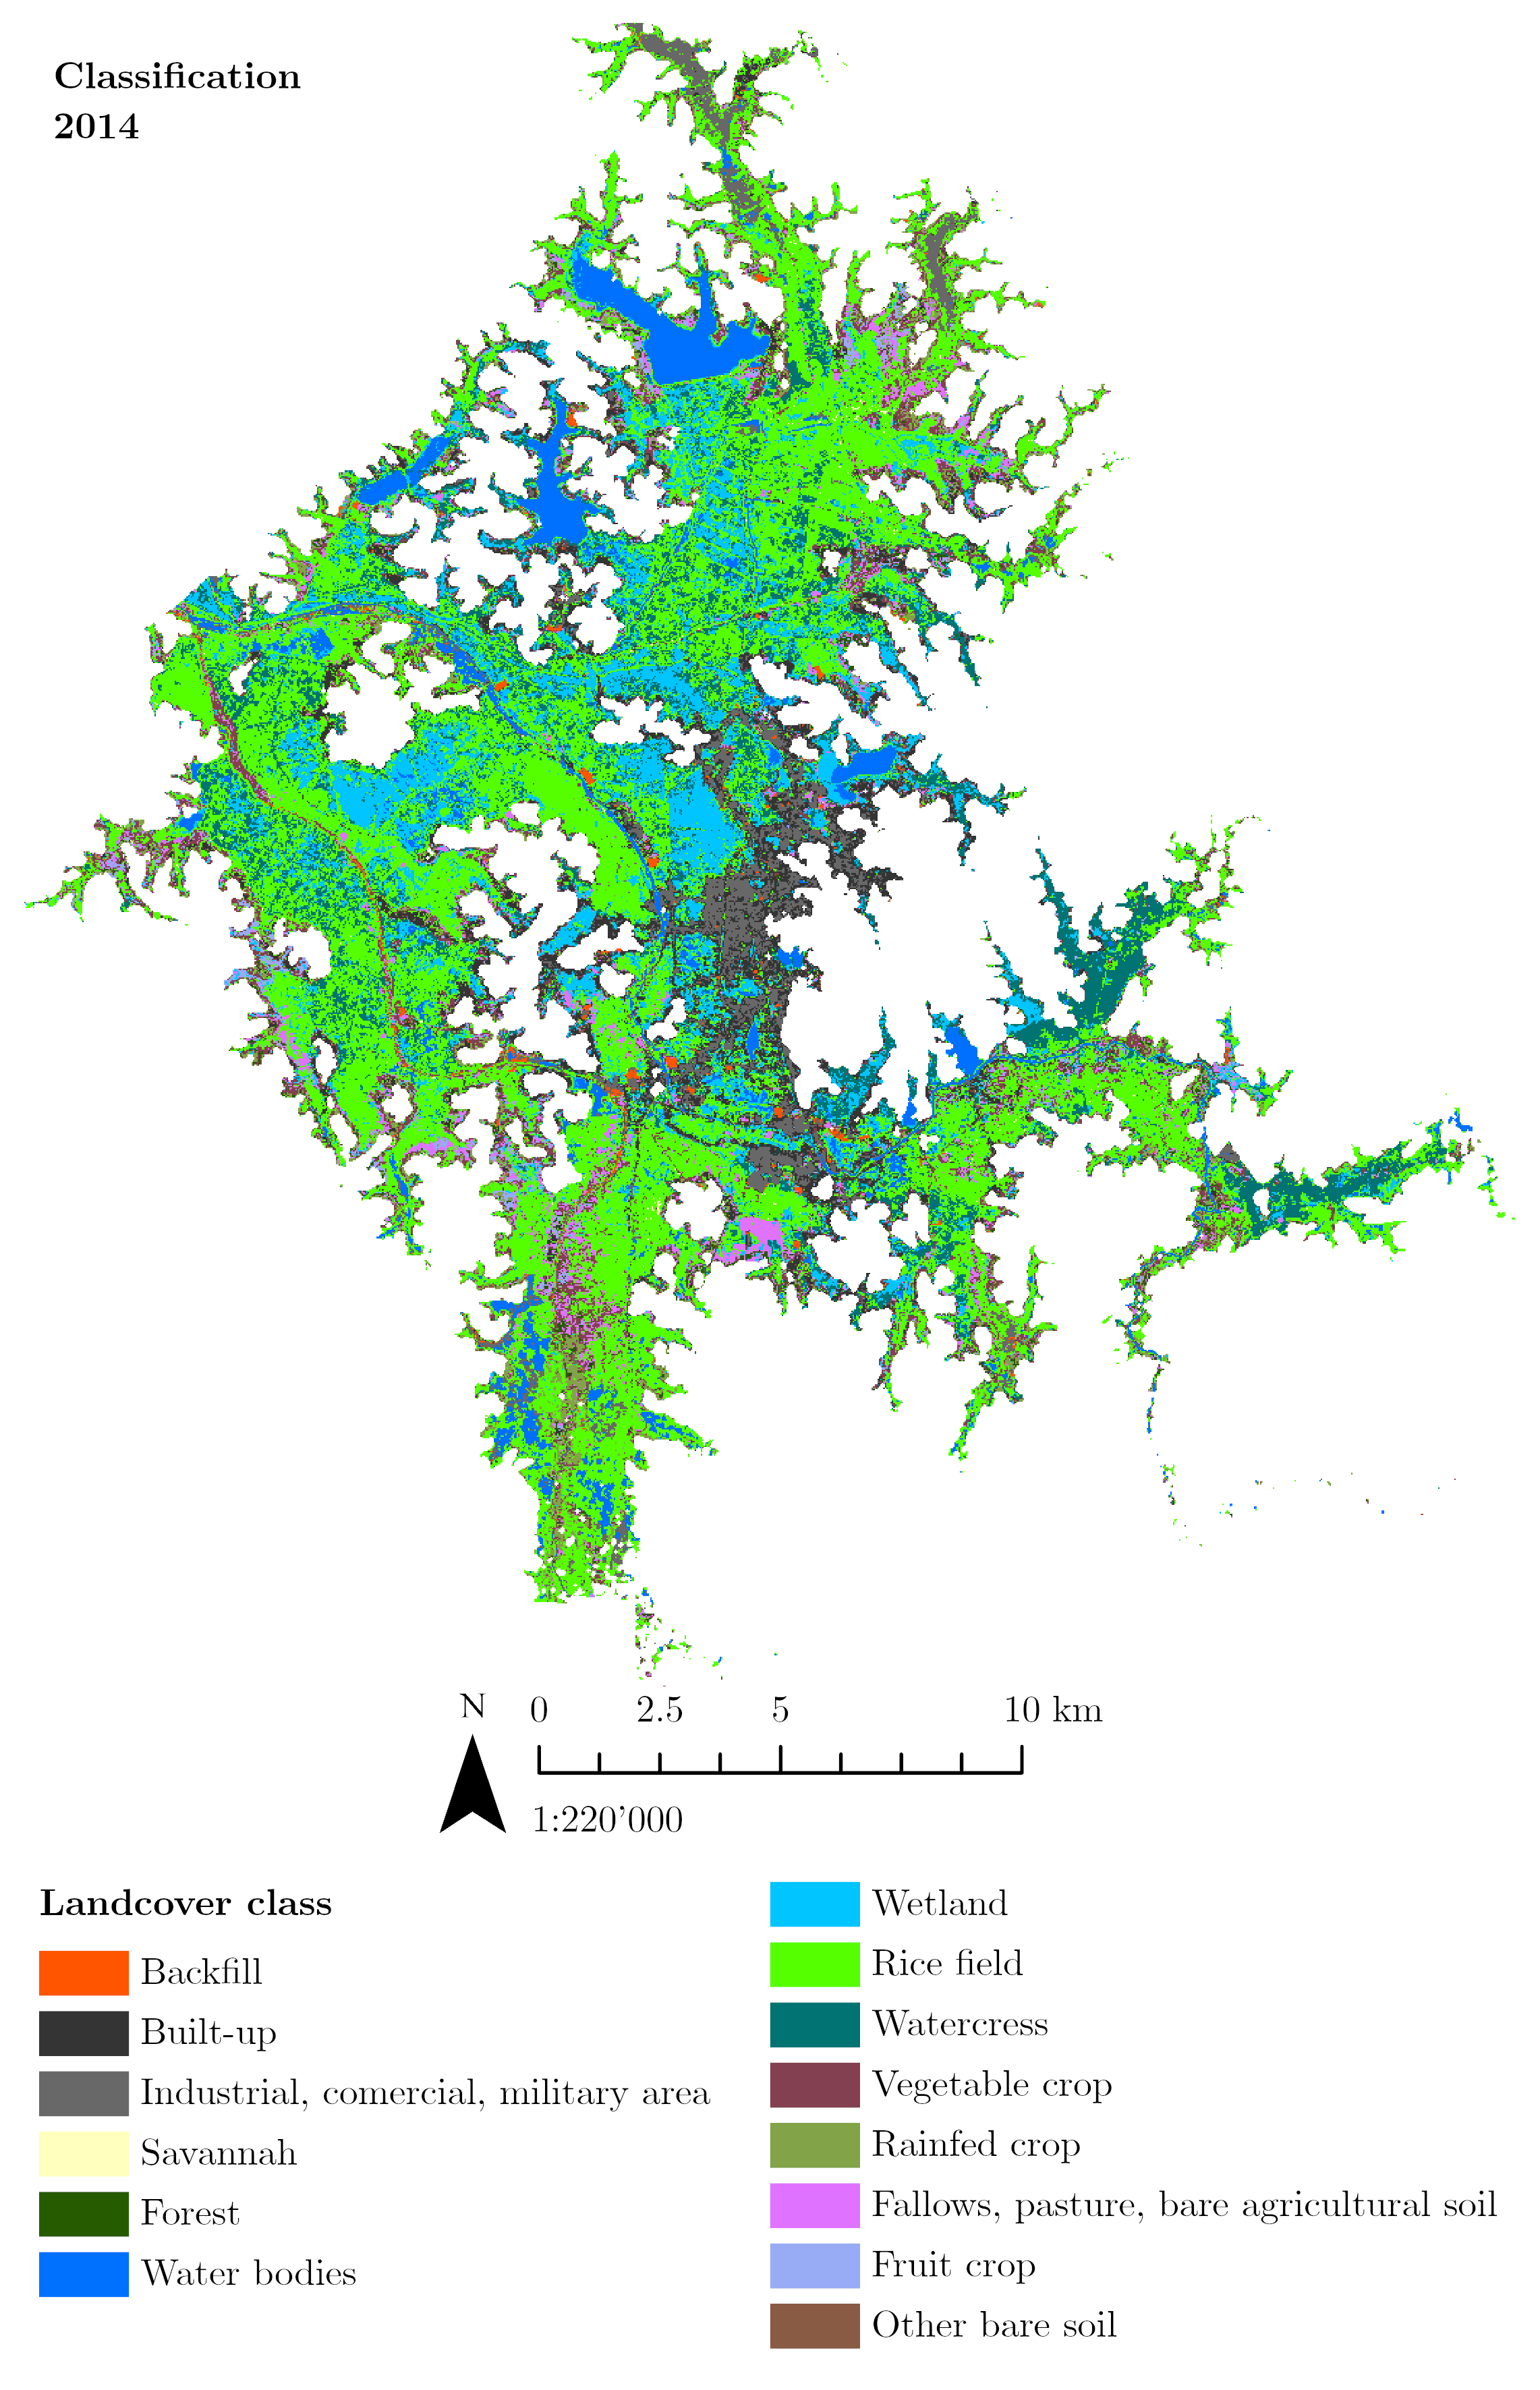
\includegraphics[width = 15cm]{figures/classi2014.png}
    \caption{Classified image resulting from the 2014 classification.}
    \label{}
\end{figure}

\begin{figure}[H]
    \centering
    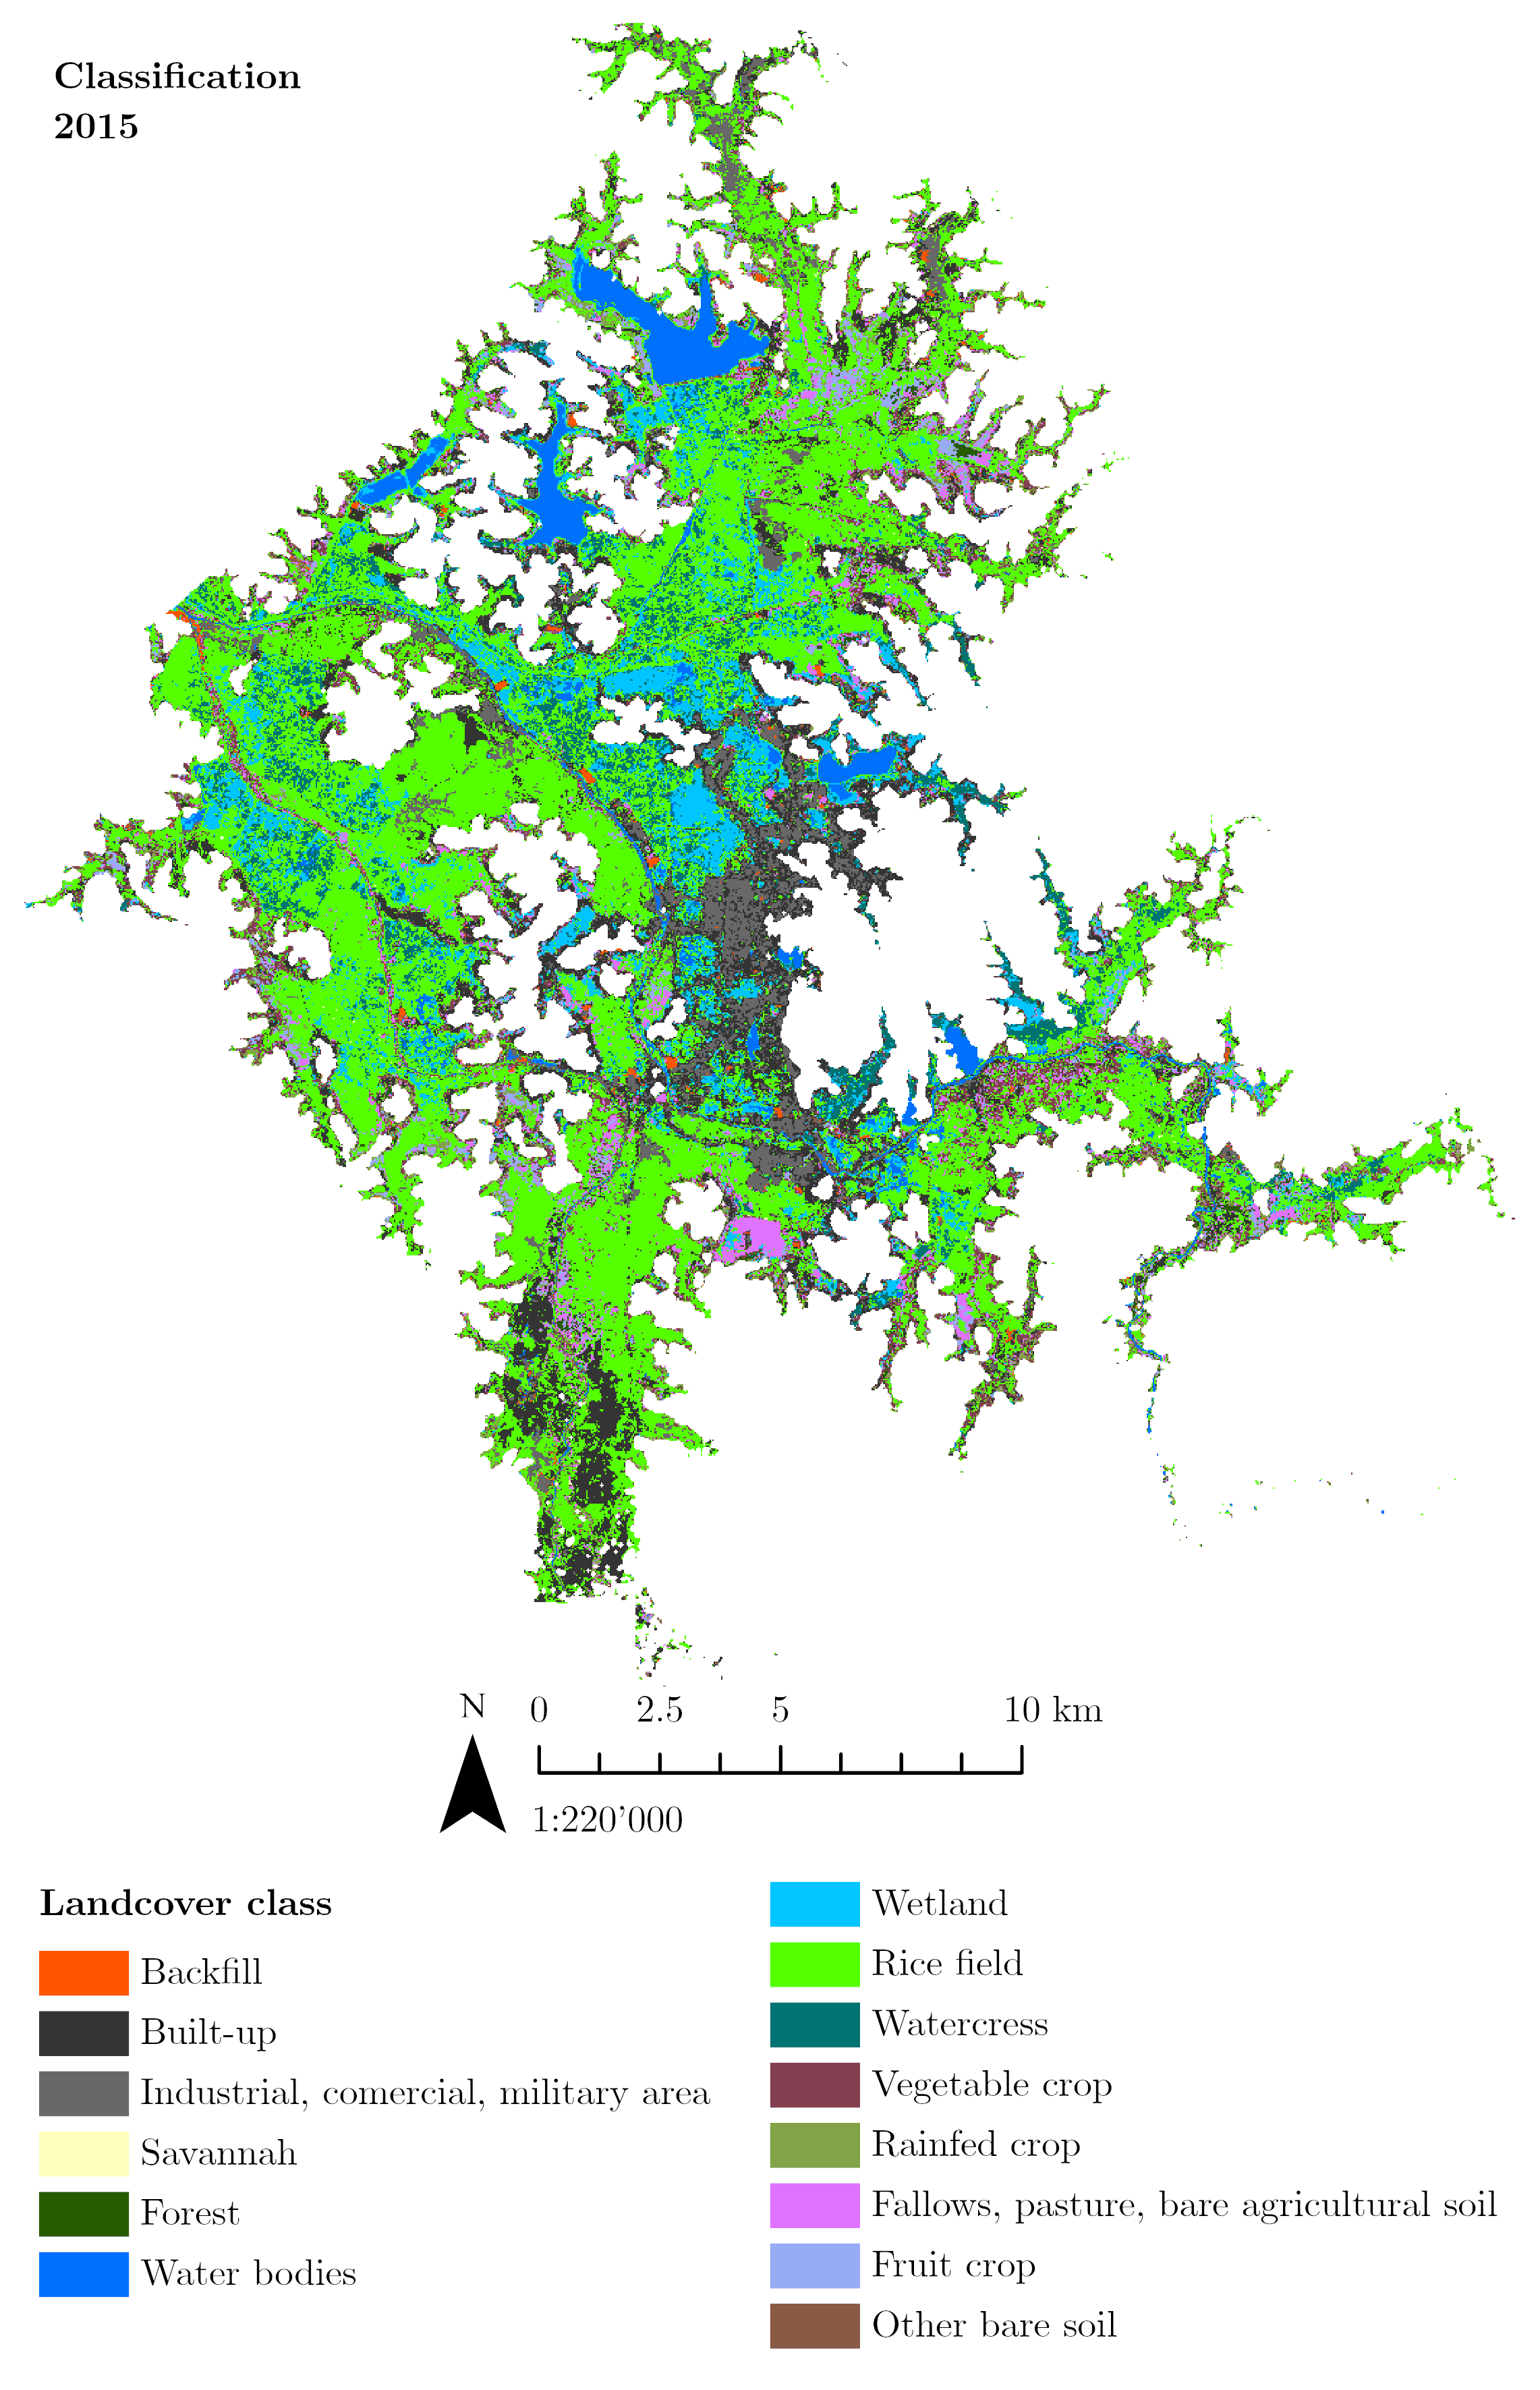
\includegraphics[width = 15cm]{figures/classi2015.png}
    \caption{Classified image resulting from the 2015 classification.}
    \label{}
\end{figure}

\begin{figure}[H]
    \centering
    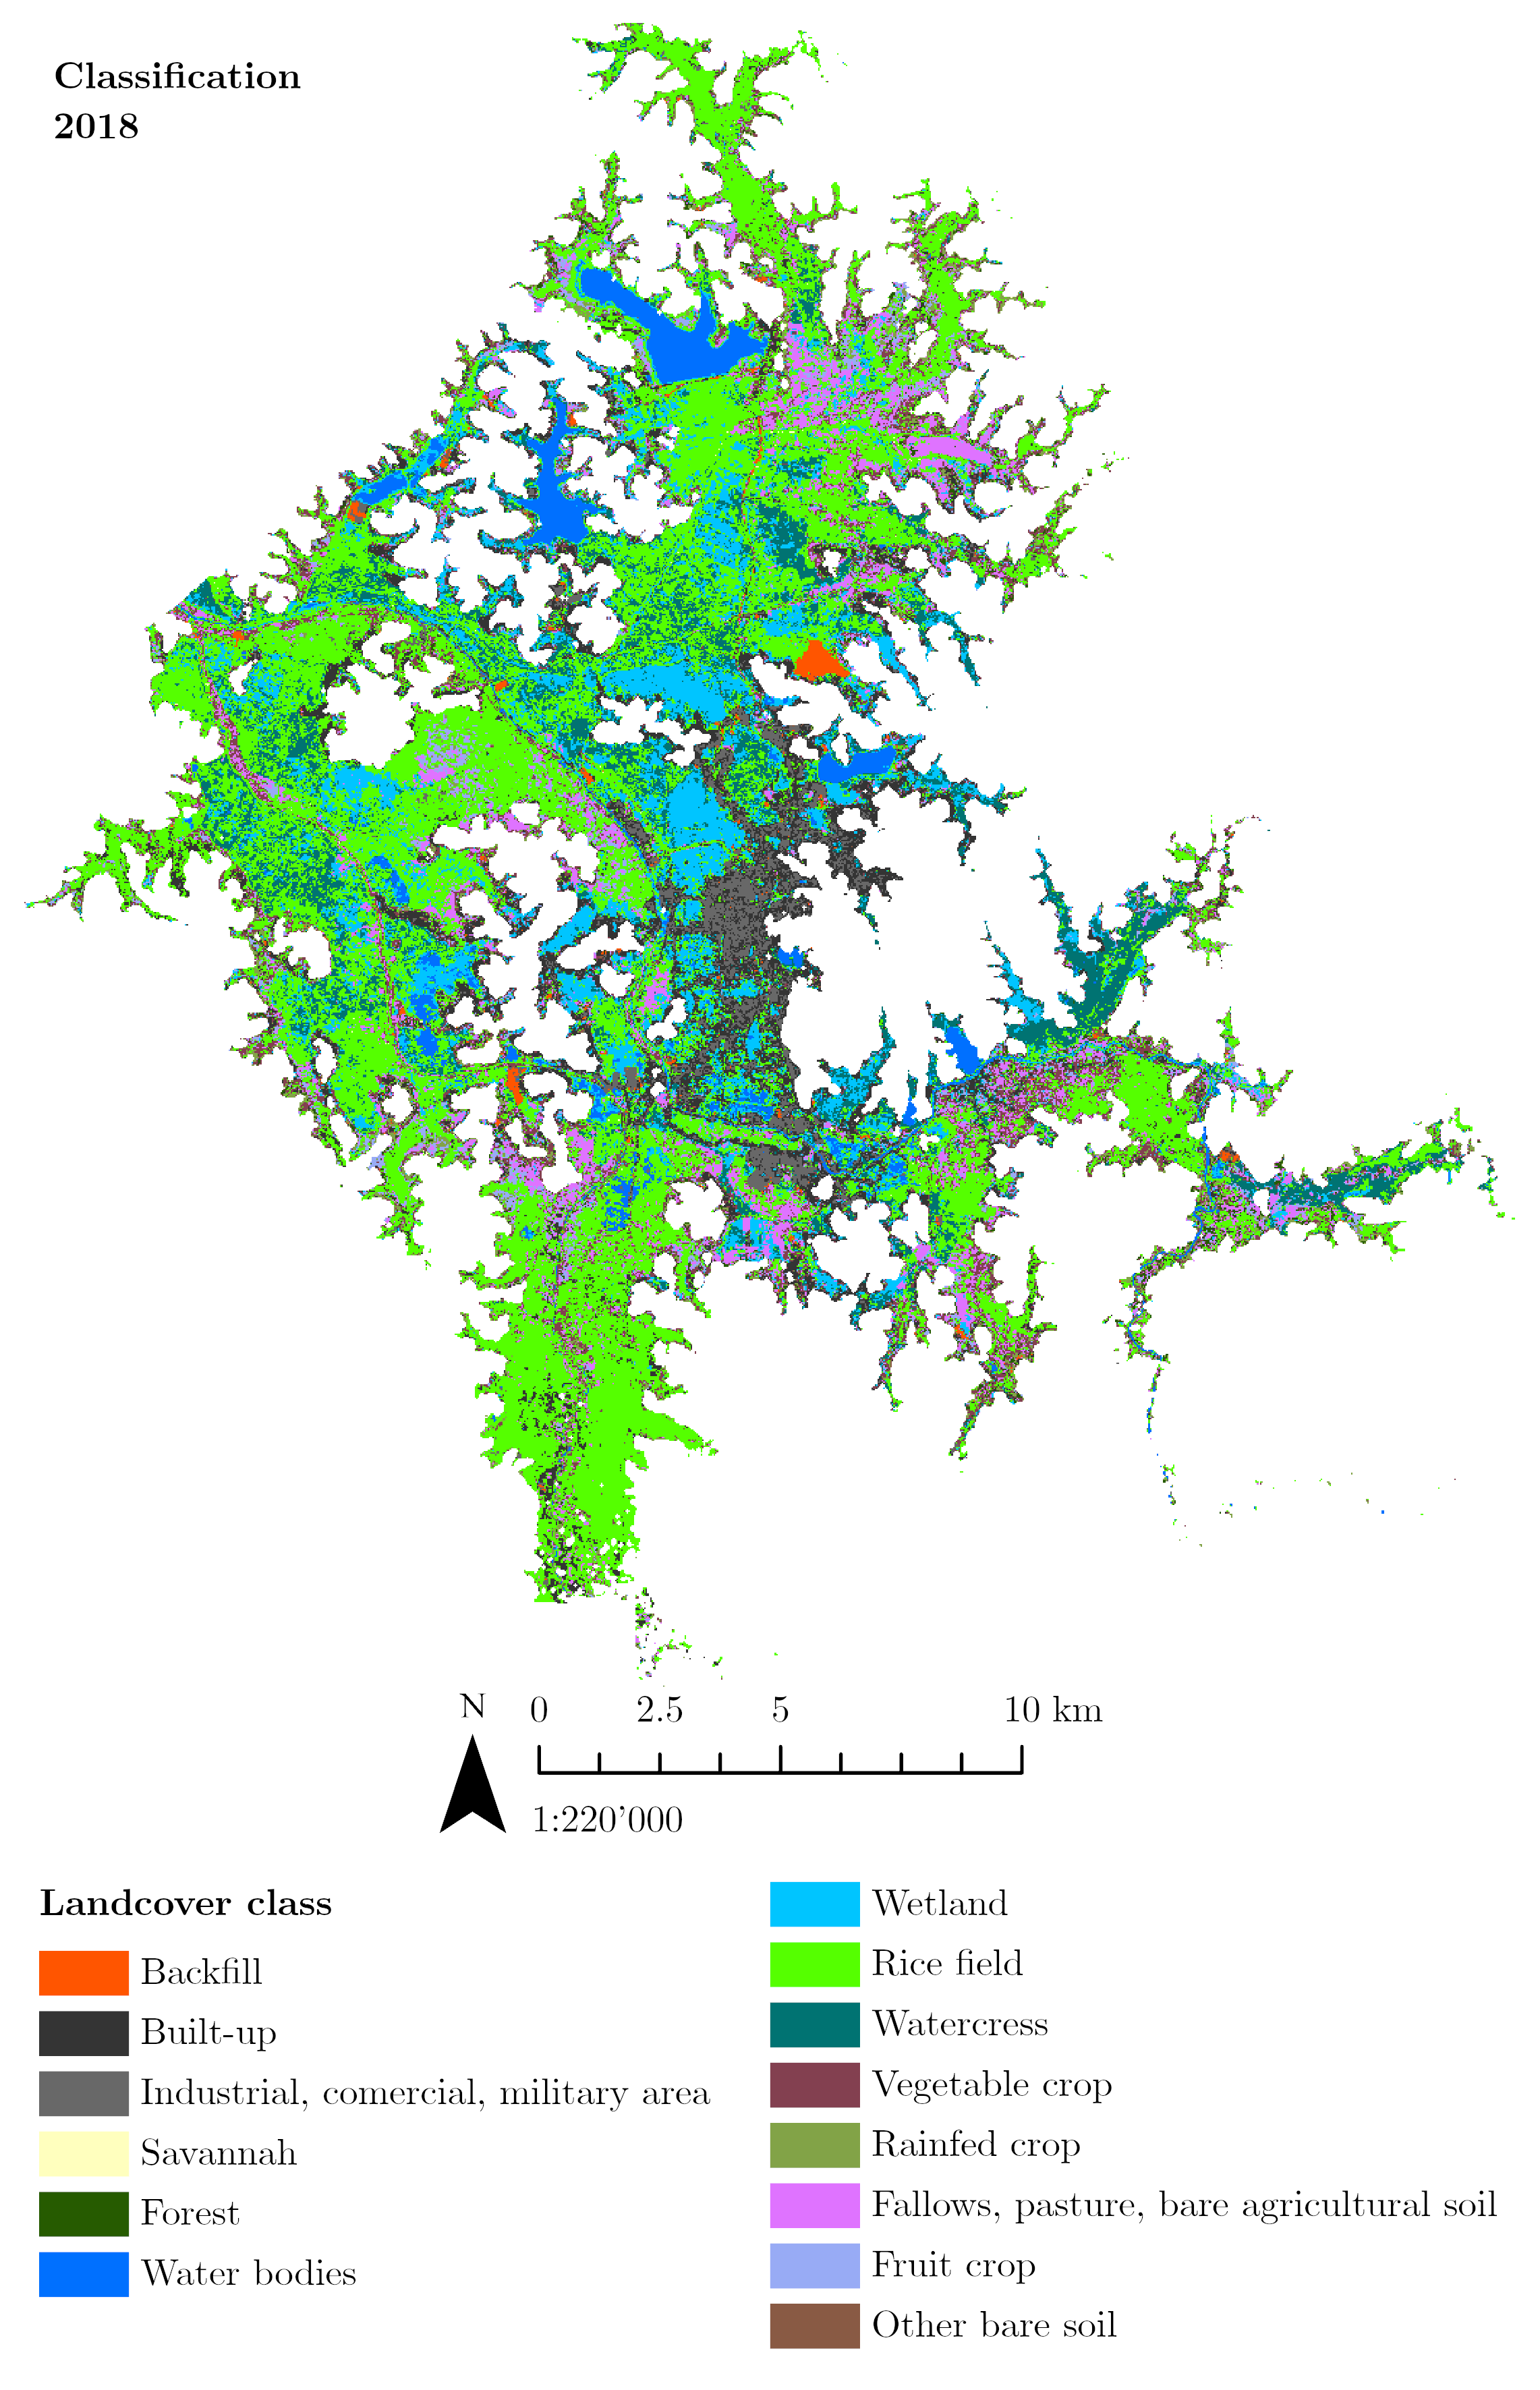
\includegraphics[width = 15cm]{figures/classi2018.png}
    \caption{Classified image resulting from the 2018 classification.}
    \label{}
\end{figure}

\begin{figure}[H]
    \centering
    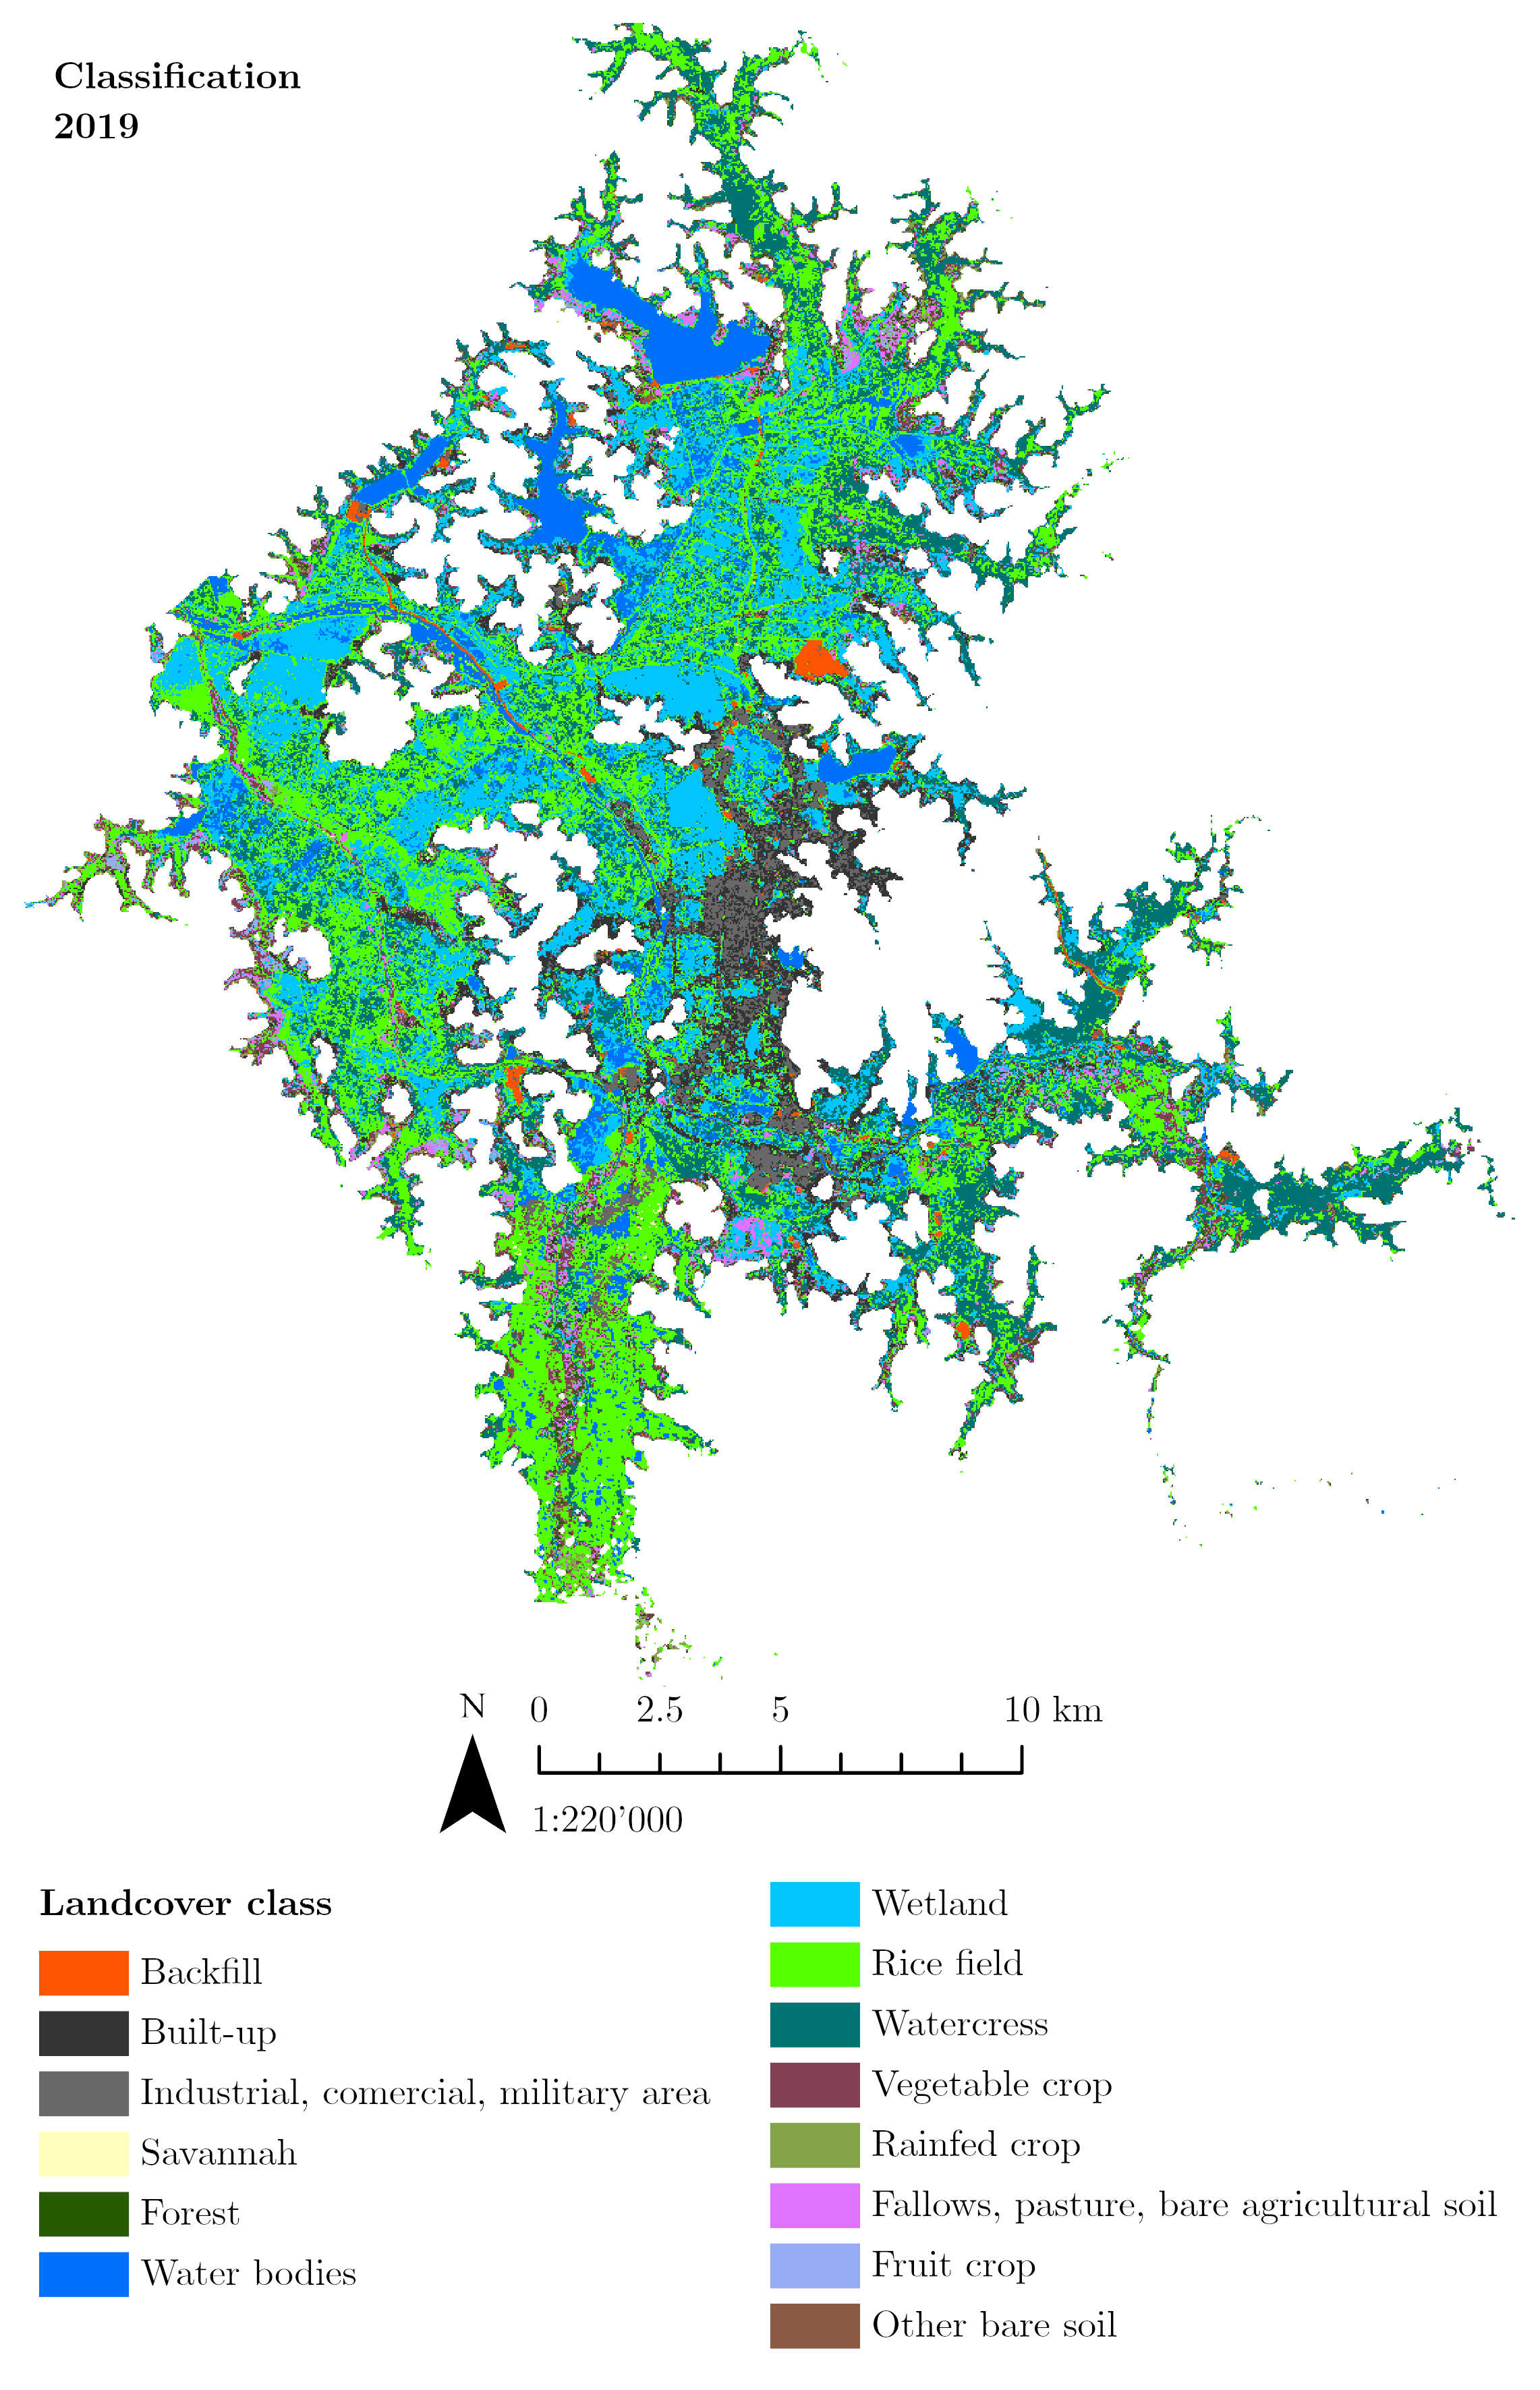
\includegraphics[width = 15cm]{figures/classi2019.png}
    \caption{Classified image resulting from the 2019 classification.}
    \label{}
\end{figure}

\begin{figure}[H]
    \centering
    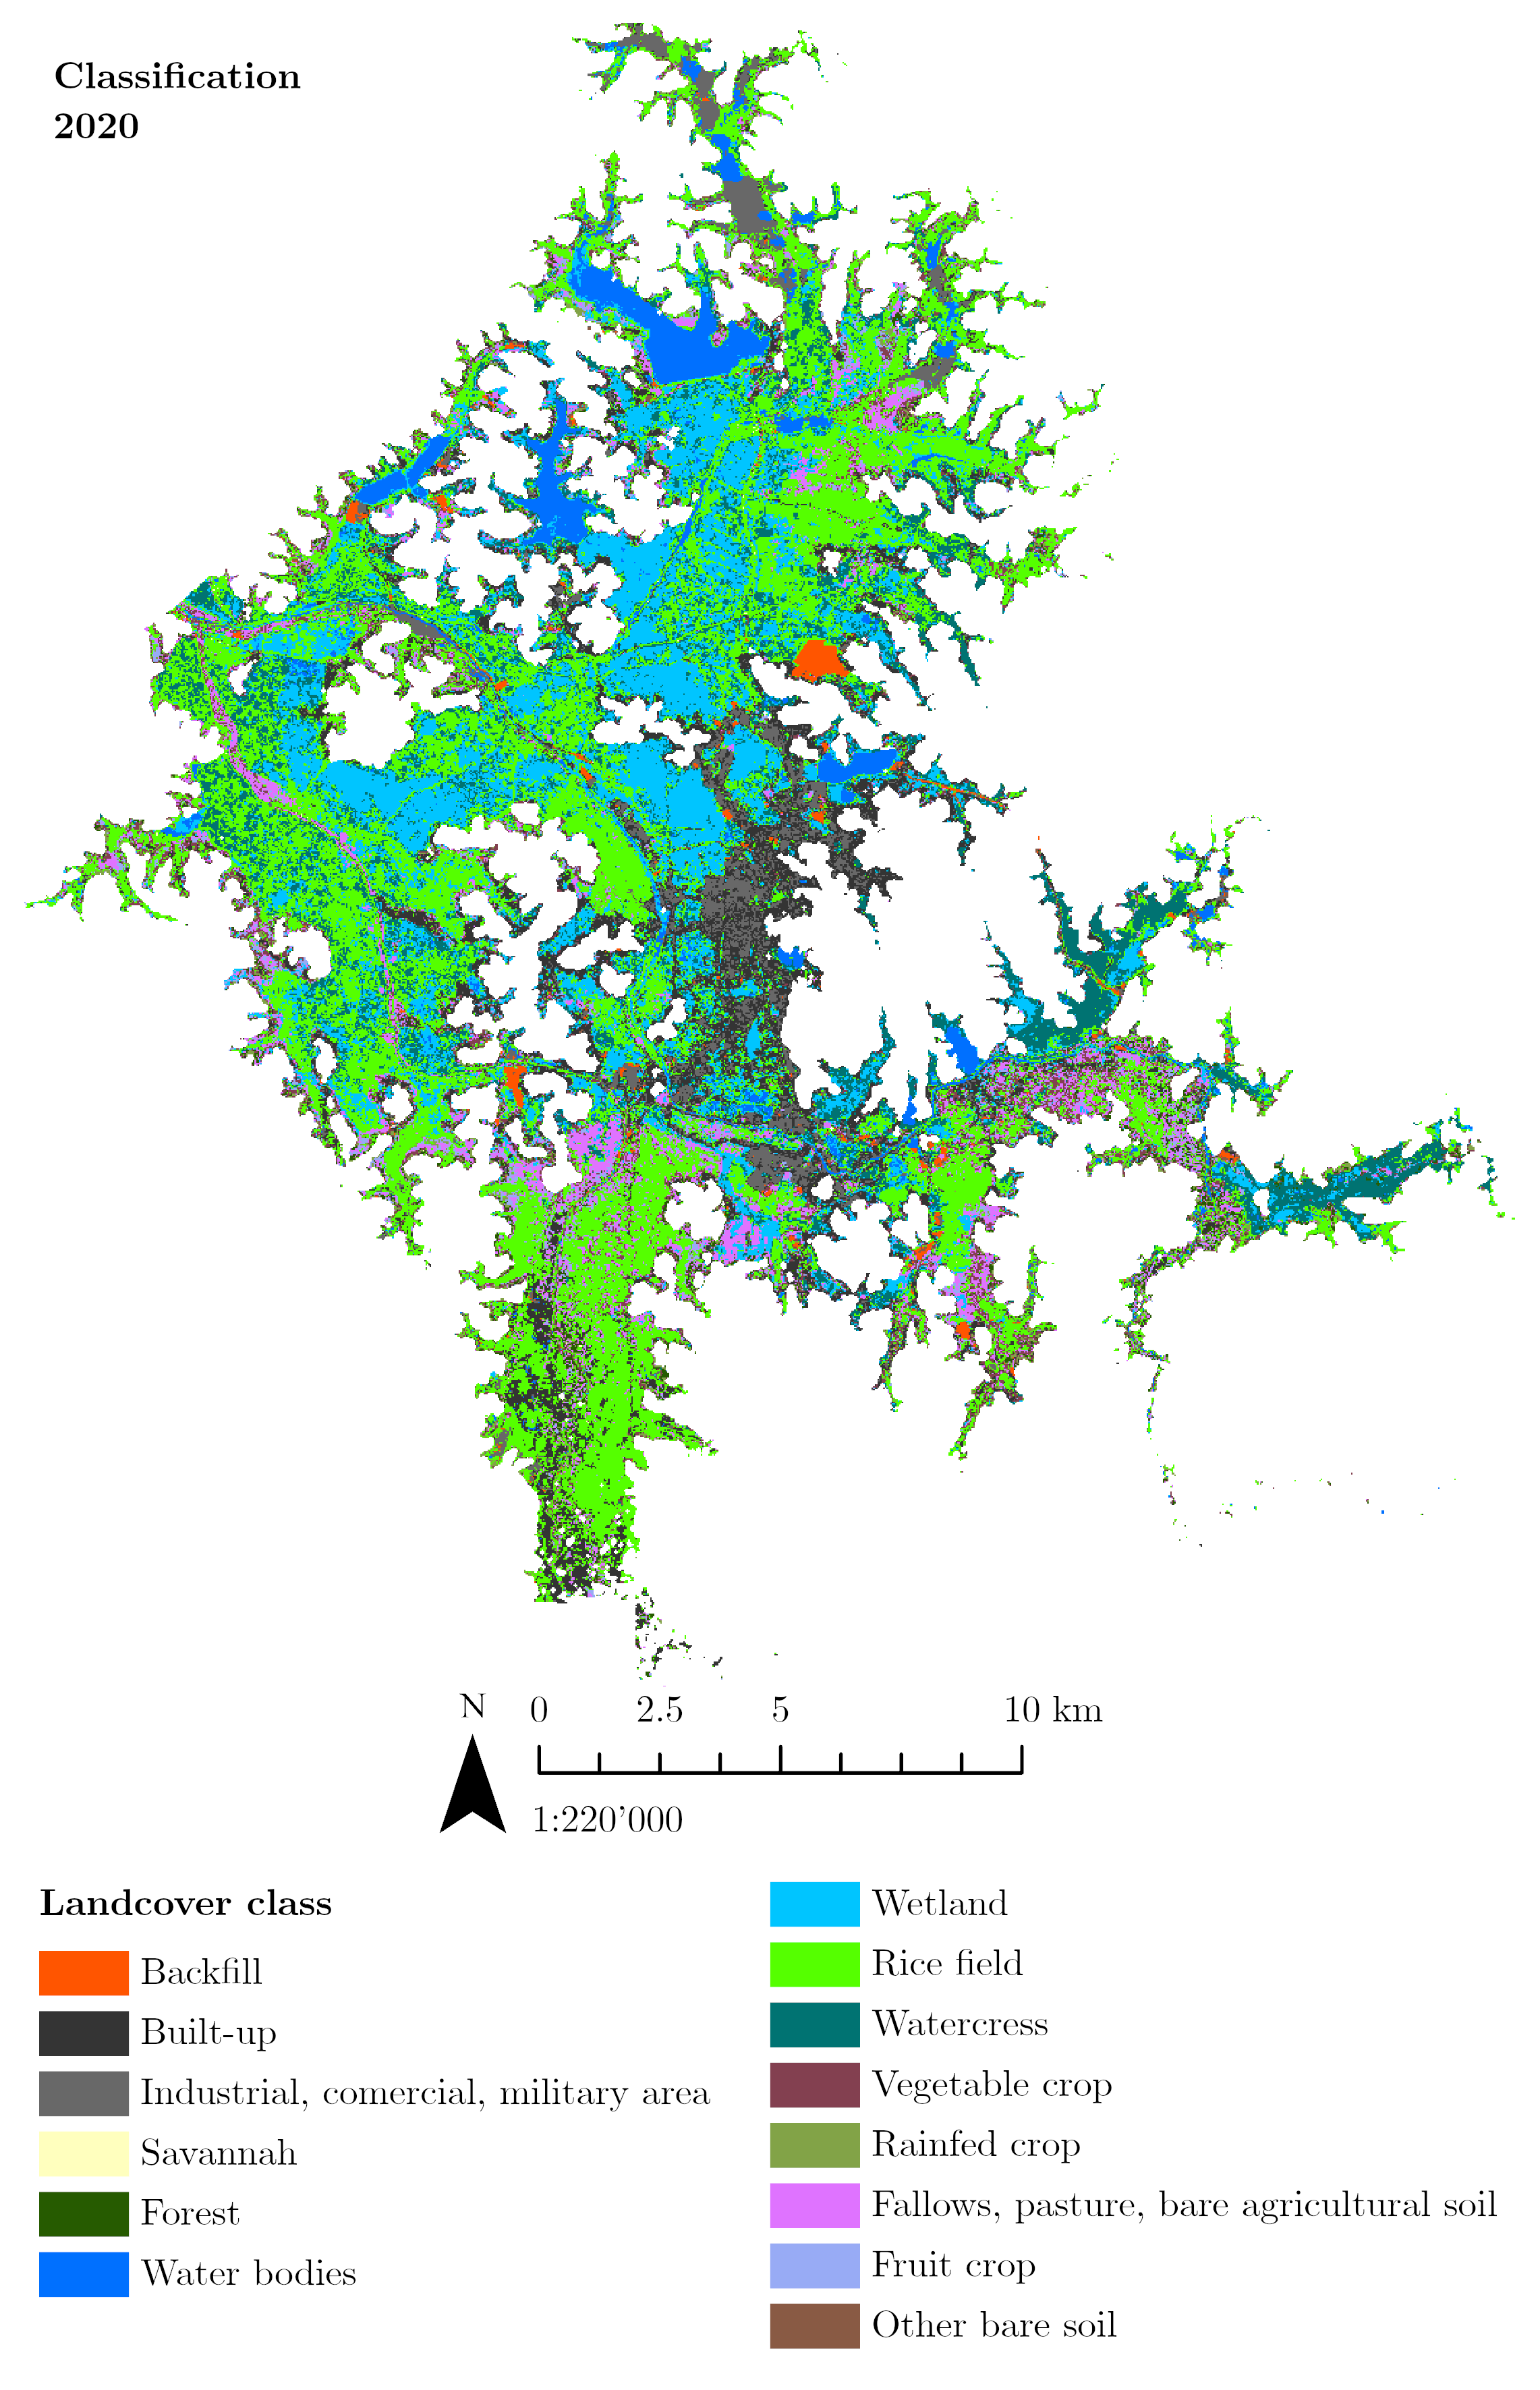
\includegraphics[width = 15cm]{figures/classi2020.png}
    \caption{Classified image resulting from the 2020 classification.}
    \label{}
\end{figure}

\begin{figure}[H]
    \centering
    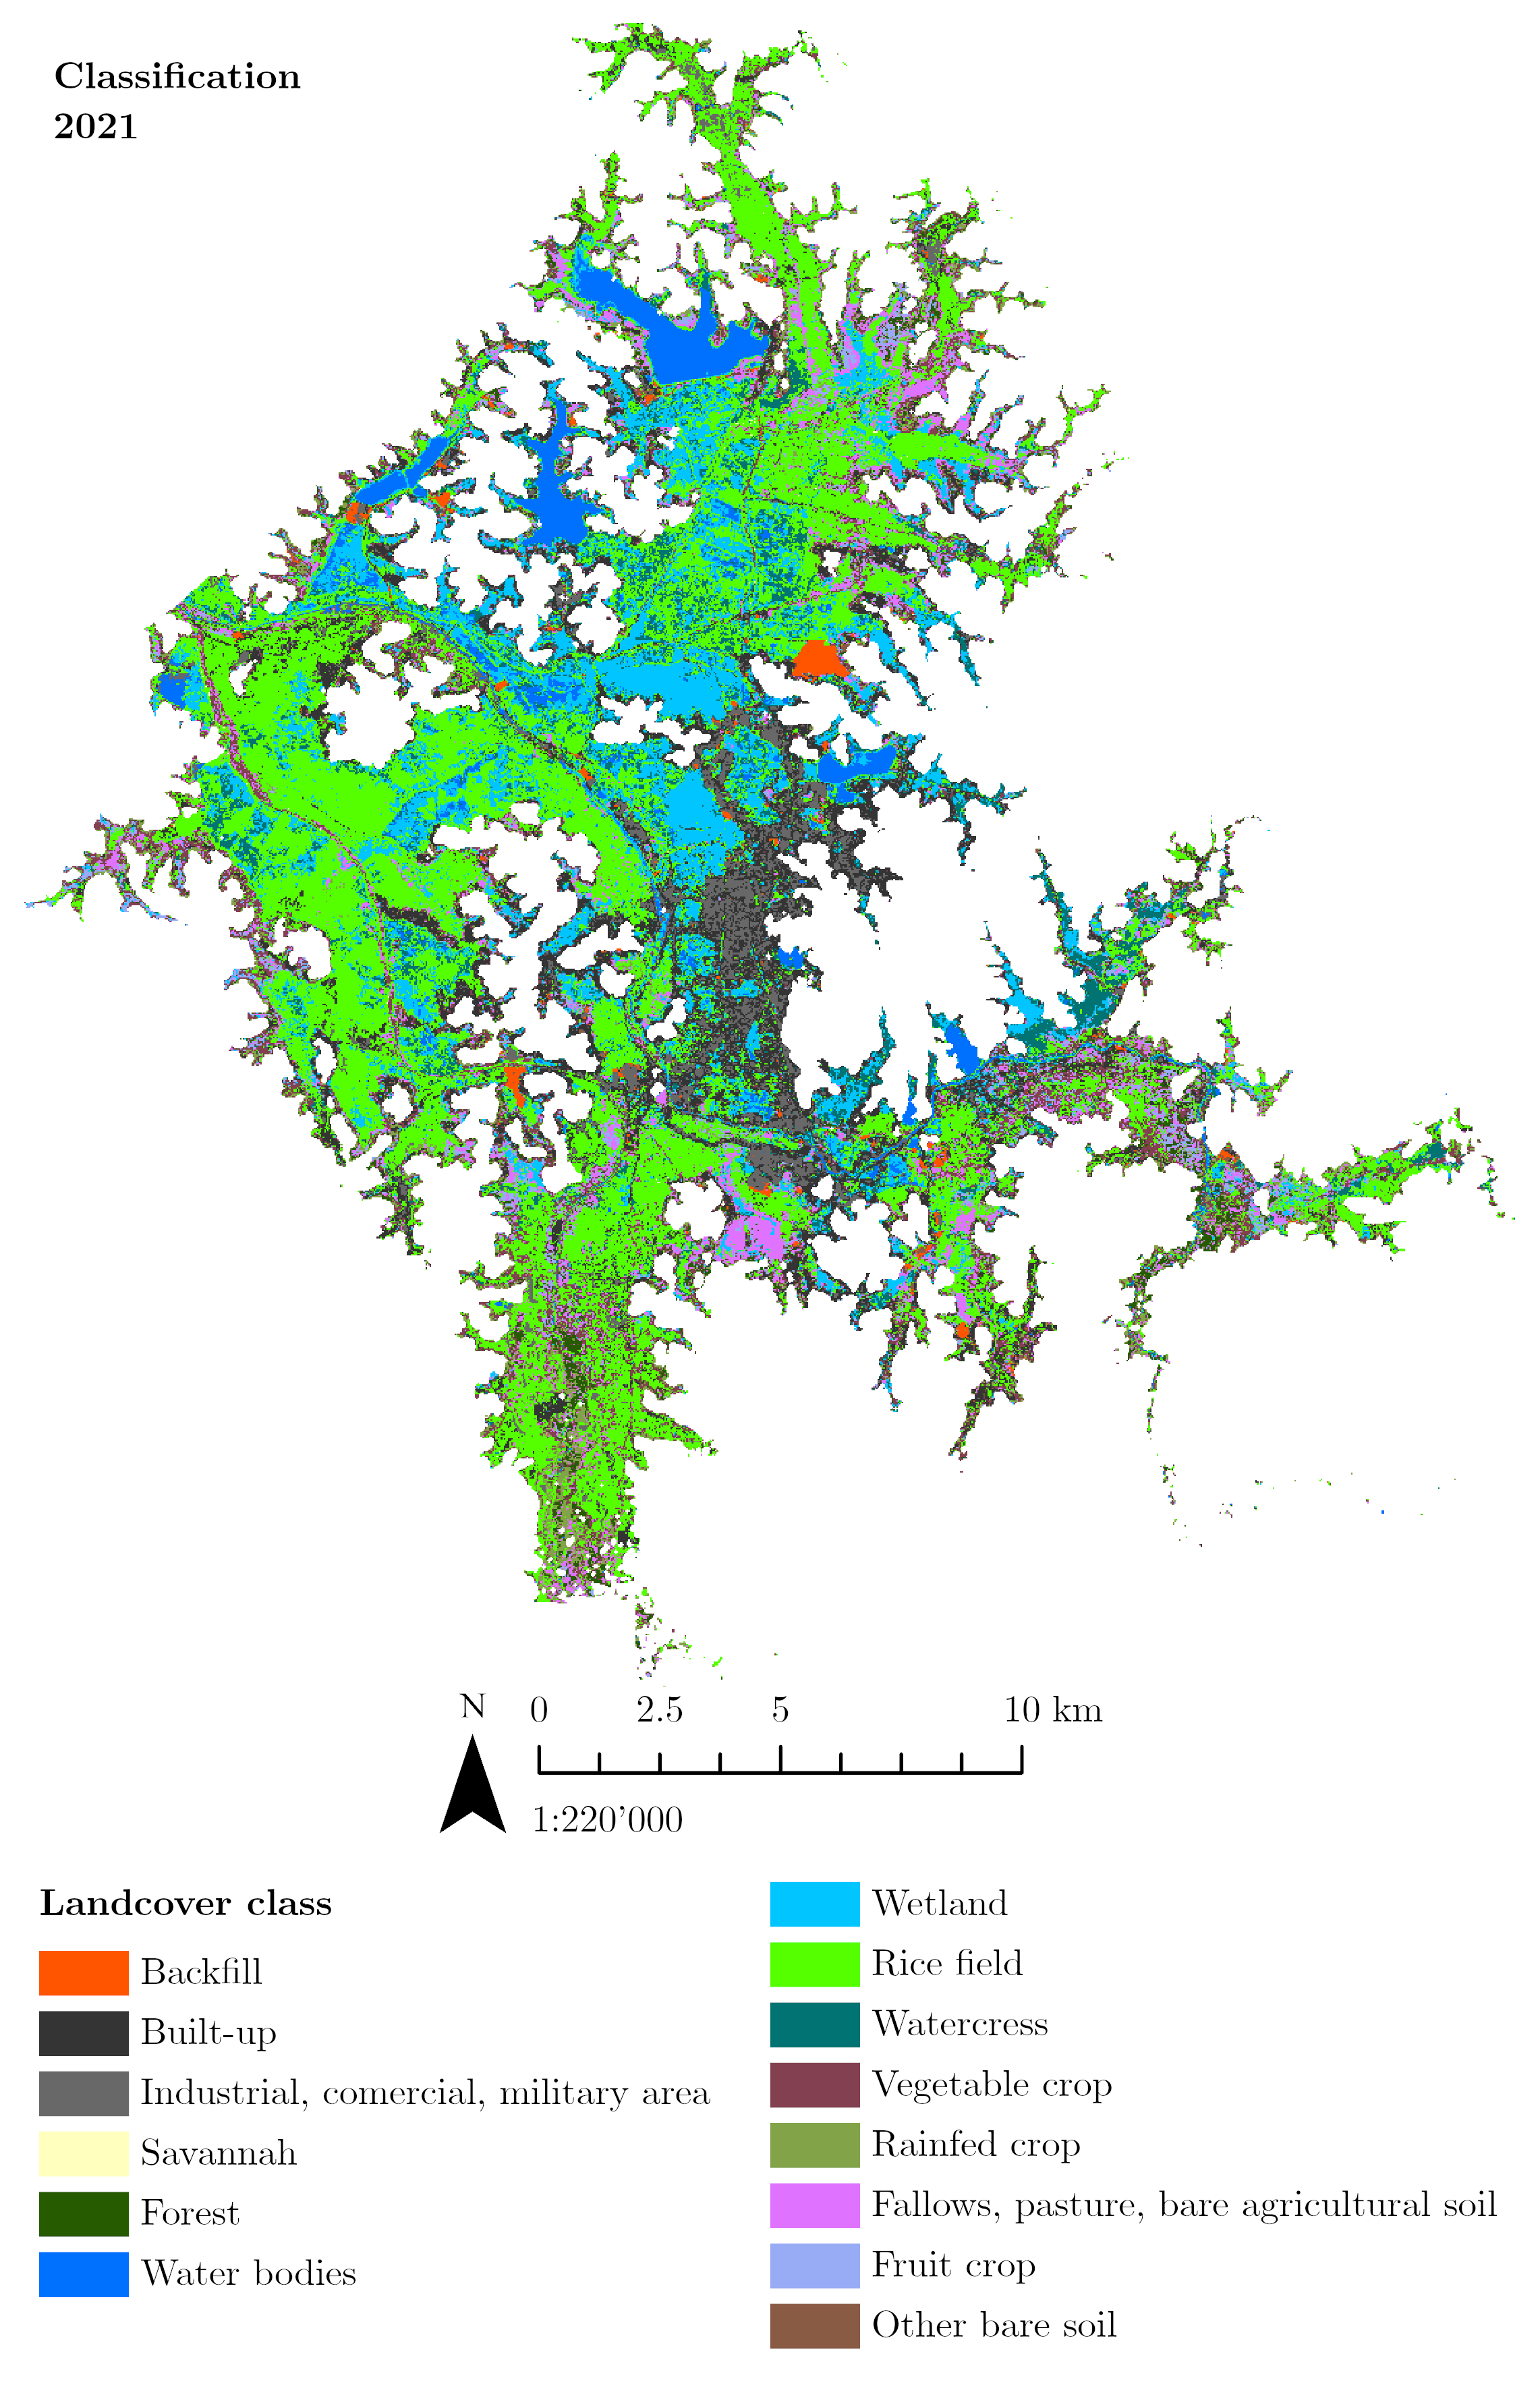
\includegraphics[width = 15cm]{figures/classi2021.png}
    \caption{Classified image resulting from the 2021 classification.}
    \label{}
\end{figure}






\begin{rotatepage}
\begin{landscape}
\begin{figure}[H]
\includegraphics[width = 25cm]{figures/north_tana.png}
\caption{Backfill area increase per year in northern Antananarivo. The data showing urban ares in the map is sourced from \citet{Dupuy.2019}.}
\label{}
\end{figure}
\end{landscape}
\end{rotatepage}


\begin{rotatepage}
\begin{landscape}
\begin{figure}[H]
\includegraphics[width = 25cm]{figures/South_Tana.png}
\caption{Backfill area increase per year in southern Antananarivo. The data showing urban ares in the map is sourced from \citet{Dupuy.2019}.}
\label{}
\end{figure}
\end{landscape}
\end{rotatepage}



\newpage
%\phantomsection
\addcontentsline{toc}{chapter}{Declaration of originality}
%\chaptertitlename{Declaration of originality}

\begin{figure}
\centering
\makebox[\textwidth]{
\includegraphics[width = 0.9\paperwidth]{D_Declaration/declaration-originality_signed.png}}
\end{figure}


\end{document}

